\documentclass[final,12pt]{colt2018} % Anonymized submission
% \documentclass{colt2017} % Include author names

% The following packages will be automatically loaded:
% amsmath, amssymb, natbib, graphicx, url, algorithm2e
 
\title[Subpolynomial trace reconstruction]{Subpolynomial trace reconstruction for random strings \\ and arbitrary deletion probability}
\usepackage{times}
\usepackage{color}
\usepackage{hyperref}
\usepackage{comment}
\usepackage[protrusion=true,expansion=true]{microtype}
\usepackage{enumerate}
\usepackage{bbm}
\usepackage{mathrsfs}
\usepackage[font=small,labelfont=bf]{caption}
\usepackage{verbatim}


\def\@rst #1 #2other{#1}
\newcommand\MR[1]{\relax\ifhmode\unskip\spacefactor3000 \space\fi
	\MRhref{\expandafter\@rst #1 other}{#1}}
\newcommand{\MRhref}[2]{\href{http://www.ams.org/mathscinet-getitem?mr=#1}{MR#2}}

\newcommand{\arXiv}[1]{\href{http://arxiv.org/abs/#1}{arXiv:#1}}
\newcommand{\arxiv}[1]{\href{http://arxiv.org/abs/#1}{#1}}

%% The following are for sans serif fonts.
\font\elevenss=cmss11
\font\tenss=cmss10
\font\niness=cmss9
\font\eightss=cmss8
\font\sevenss=cmss8 at 7pt
\font\sixss=cmss8 at 6pt
\font\fivess=cmss8 at 5pt
\newfam\ssfam
\textfont\ssfam=\elevenss \scriptfont\ssfam=\eightss
\scriptscriptfont\ssfam=\sixss
\def\ss{\fam\ssfam \elevenss}%


\def\MR#1{\href{http://www.ams.org/mathscinet-getitem?mr=#1}{MR#1}}


\newtheorem*{unremark}{Remark}
\newtheorem*{unremarks}{Remarks}

\renewcommand{\bottomfraction}{0.97}

\newcommand{\B}{\mathbbm{B}}
\newcommand{\C}{\mathbbm{C}}
\newcommand{\D}{\mathbbm{D}}
\newcommand{\E}{\mathbbm{E}}
\newcommand{\N}{\mathbbm{N}}
\newcommand{\Nz}{\mathbbm{N}_0}
\newcommand{\Q}{\mathbbm{Q}}
\newcommand{\Z}{\mathbbm{Z}}
\newcommand{\R}{\mathbbm{R}}
\renewcommand{\P}{\mathbbm{P}}
\newcommand{\bbH}{\mathbbm{H}}

\newcommand{\eps}{\varepsilon}
\newcommand{\1}{\mathbf{1}}
\newcommand{\one}{\mathbf{1}}
\renewcommand{\Re}{\mathrm{Re}}
\renewcommand{\Im}{\mathrm{Im}}

\newcommand{\scr}{\mathscr}

\DeclareMathOperator{\dit}{dist}
\DeclareMathOperator{\diam}{diam}
\DeclareMathOperator{\supp}{supp}
\DeclareMathOperator{\har}{har}
\DeclareMathOperator{\GFF}{GFF}
\DeclareMathOperator{\Cov}{Cov}
\DeclareMathOperator{\Var}{Var}
\DeclareMathOperator{\SLE}{SLE}
\DeclareMathOperator{\CLE}{CLE}

\def\disp{\displaystyle}
\def\cZ{\mathcal{Z}}
\def\cY{\mathcal{Y}}
\def\cX{\mathcal{X}}
\def\cW{\mathcal{W}}
\def\cV{\mathcal{V}}
\def\cU{\mathcal{U}}
\def\cT{\mathcal{T}}
\def\cS{\mathcal{S}}
\def\cSS{\frak{S}}
\def\cR{\mathcal{R}}
\def\cQ{\mathcal{Q}}
\def\cP{\mathcal{P}}
\def\cO{\mathcal{O}}
\def\cN{\mathcal{N}}
\def\cM{\mathcal{M}}
\def\cL{\mathcal{L}}
\def\cK{\mathcal{K}}
\def\cJ{\mathcal{J}}
\def\cI{\mathcal{I}}
\def\cH{\mathcal{H}}
\def\cG{\mathcal{G}}
\def\cF{\mathcal{F}}
\def\cE{\mathcal{E}}
\def\cD{\mathcal{D}}
\def\cC{\mathcal{C}}
\def\cB{\mathcal{B}}
\def\cA{\mathcal{A}}
\def\cS{\mathcal{S}}
\def\cl{\mathfrak{l}}
\def\Cox{\hfill \Box}

\newcommand{\aryb}{\begin{eqnarray*}}
	\newcommand{\arye}{\end{eqnarray*}}
\def\alb#1\ale{\begin{align*}#1\end{align*}}
\newcommand{\eqb}{\begin{equation}}
\newcommand{\eqe}{\end{equation}}
\newcommand{\eqbn}{\begin{equation*}}
\newcommand{\eqen}{\end{equation*}}

\newcommand{\BB}{\mathbbm}
\newcommand{\ol}{\overline}
\newcommand{\ul}{\underline}
\newcommand{\op}{\operatorname}
\newcommand{\la}{\langle}
\newcommand{\ra}{\rangle}
\newcommand{\bd}{\mathbf}
\newcommand{\im}{\operatorname{Im}}
\newcommand{\re}{\operatorname{Re}}
\newcommand{\frk}{\mathfrak}
\newcommand{\eqD}{\overset{d}{=}}
\newcommand{\rtaD}{\overset{d}{\rightarrow}}
\newcommand{\ep}{\epsilon}
\newcommand{\rta}{\rightarrow}
\newcommand{\xrta}{\xrightarrow}
\newcommand{\Rta}{\Rightarrow}
\newcommand{\hookrta}{\hookrightarrow}
\newcommand{\wt}{\widetilde}
\newcommand{\wh}{\widehat}
\newcommand{\mcl}{\mathcal}
\newcommand{\pre}{{\operatorname{pre}}}
\newcommand{\lrta}{\leftrightarrow}
\newcommand{\bdy}{\partial}

\def\Pt{{\wt{P}}}
\def\Qt{{\wt{Q}}}
\def\aat{{\wt{a}}}
\def\xt{{\wt {\bf x}}}
\def\wtt{{\wt {\bf w}}}
\def\khat{{\wh k}}
\def\x{{\bf x}}
\def\y{{\bf y}}
\def\at{{\wt {\bf a}}}
\def\a{{\bf a}}
\def\w{{\bf w}}
\def\ratio{\beta}
\def\indep{{\bf Q}}
\def\ee{\varepsilon}
\def\csep{C_{\rm sep}} %the constant we can't control, \Ct_2
\def\cfwd{C_{\rm fwd}} %another constant we can't control, \Ct_3
%\def\cback{C_1}
%\def\calign{C_2}
%\def\ctrue{C_3}
%\def\cfalse{C_4}
%\def\cavg{C_5}
\def\cback{C_{\rm back}}
\def\calign{C_{\rm align}}
\def\ctrue{C_{\rm true}}
\def\cfalse{C_{\rm false}}
\def\cavg{C_{\rm avg}}
\def\cbe{C_{\rm BE}}
\def\cm{C_m}
\def\crw{C_{\rm RW}}
\def\ct{{\wt c}}
\def\chuge{C_{\rm BIG}}
\def\Rhat{{\mathcal Q}}
\def\Rc{{\mathcal H}}
\def\shat{\hat{\sigma}}
\def\bad{{\Xi_{\rm bad}}}
\def\rapid{{\mathfrak r}}
\def\Bin{{\rm Bin}\,}
\def\nubar{\overline{g}}
\def\nubarh{\overline{h}}
\def\sign{\op{sign}}
\def\good{{\ss GOOD}}
\def\rough{{\rho}}
\def\CC{{\mathcal C}}


\newcommand{\nina}[1]{{\color{red}{#1}}}
\newcommand{\robin}[1]{{\color{cyan}{#1}}}

\DeclareMathAlphabet{\mathpzc}{OT1}{pzc}{m}{it}

 % Use \Name{Author Name} to specify the name.
 % If the surname contains spaces, enclose the surname
 % in braces, e.g. \Name{John {Smith Jones}} similarly
 % if the name has a "von" part, e.g \Name{Jane {de Winter}}.
 % If the first letter in the forenames is a diacritic
 % enclose the diacritic in braces, e.g. \Name{{\'E}louise Smith}

 % Two authors with the same address
  % \coltauthor{\Name{Author Name1} \Email{abc@sample.com}\and
  %  \Name{Author Name2} \Email{xyz@sample.com}\\
  %  \addr Address}

 % Three or more authors with the same address:
 % \coltauthor{\Name{Author Name1} \Email{an1@sample.com}\\
 %  \Name{Author Name2} \Email{an2@sample.com}\\
 %  \Name{Author Name3} \Email{an3@sample.com}\\
 %  \addr Address}


 % Authors with different addresses:
 \coltauthor{\Name{Nina Holden} \Email{ninah$@$math.mit.edu}\\
 \addr Department of Mathematics, Massachusetts Institute of Technology, Cambridge, MA %02139%-4307
 \AND
 \Name{Robin Pemantle} \Email{pemantle$@$math.upenn.edu}\\
 \addr Department of Mathematics, University of Pennsylvania, Philadelphia, PA %19104%-6395
 \AND
 \Name{Yuval Peres} \Email{peres$@$microsoft.com}\\
 \addr Microsoft Research, Redmond, WA%, 98052 
 }



\begin{document}

\maketitle

\begin{abstract}
The deletion-insertion channel takes as input a bit string $\x\in
\{0,1\}^{n}$, and outputs a string where bits have been deleted and inserted independently at random. The trace reconstruction problem is to recover $\x$ from many independent outputs (called ``traces'') of the deletion-insertion channel applied to $\x$. We show that if $\x$ is chosen uniformly at random, then $\exp(O(\log^{1/3} n))$ traces suffice to reconstruct $\x$ with high probability. For the deletion channel with deletion probability $q<1/2$ the earlier upper bound was $\exp(O(\log^{1/2} n))$. The case of $q\geq 1/2$ or the case where insertions are allowed has not been previously analysed, and therefore the earlier upper bound was as for worst-case strings, i.e., $\exp(O( n^{1/3}))$.
 
A key ingredient in our proof is a delicate two-step alignment procedure where we estimate the location in each trace corresponding to a given bit of $\x$. The alignment is done by viewing the strings as random walks, and comparing the increments in the walk associated with the input string and the trace, respectively.
\end{abstract}

\begin{keywords}
	Trace reconstruction;  Deletion channel; Sample complexity.  
\end{keywords}

\vspace{\baselineskip}

Learning a parameter from a sequence of noisy observations is a basic problem in statistical inference and machine learning. The amount of data  required (known as the {\em sample complexity}) to learn the parameter is of fundamental interest.  A natural problem in this class where the missing parameter is a bit string and it is unknown whether the sample complexity is polynomial, is the trace reconstruction problem for   the {\bf deletion-insertion channel}. This channel takes as input a string
$\x=(x_0,x_1,\dots,x_{n-1}) \in \{0,1\}^{n}$ and outputs a noisy
version of it, where bits have been randomly inserted and deleted. Let $q\in[0,1)$ be the deletion probability and let $q'\in[0,1)$ be the insertion probability. First, for each $j$, before the $j$th bit of $\x$ we insert $G_j-1$ uniform and
independent bits, where the independent geometric random variables $G_j \ge 1 $ have parameter
$1-q'$. Then we delete each bit of the resulting string independently with probability $q$.
The output string $\xt$ is called a {\bf trace}.  An example is shown in Figure~\ref{fig:trace}.

\begin{figure}[ht!]
	\centering
	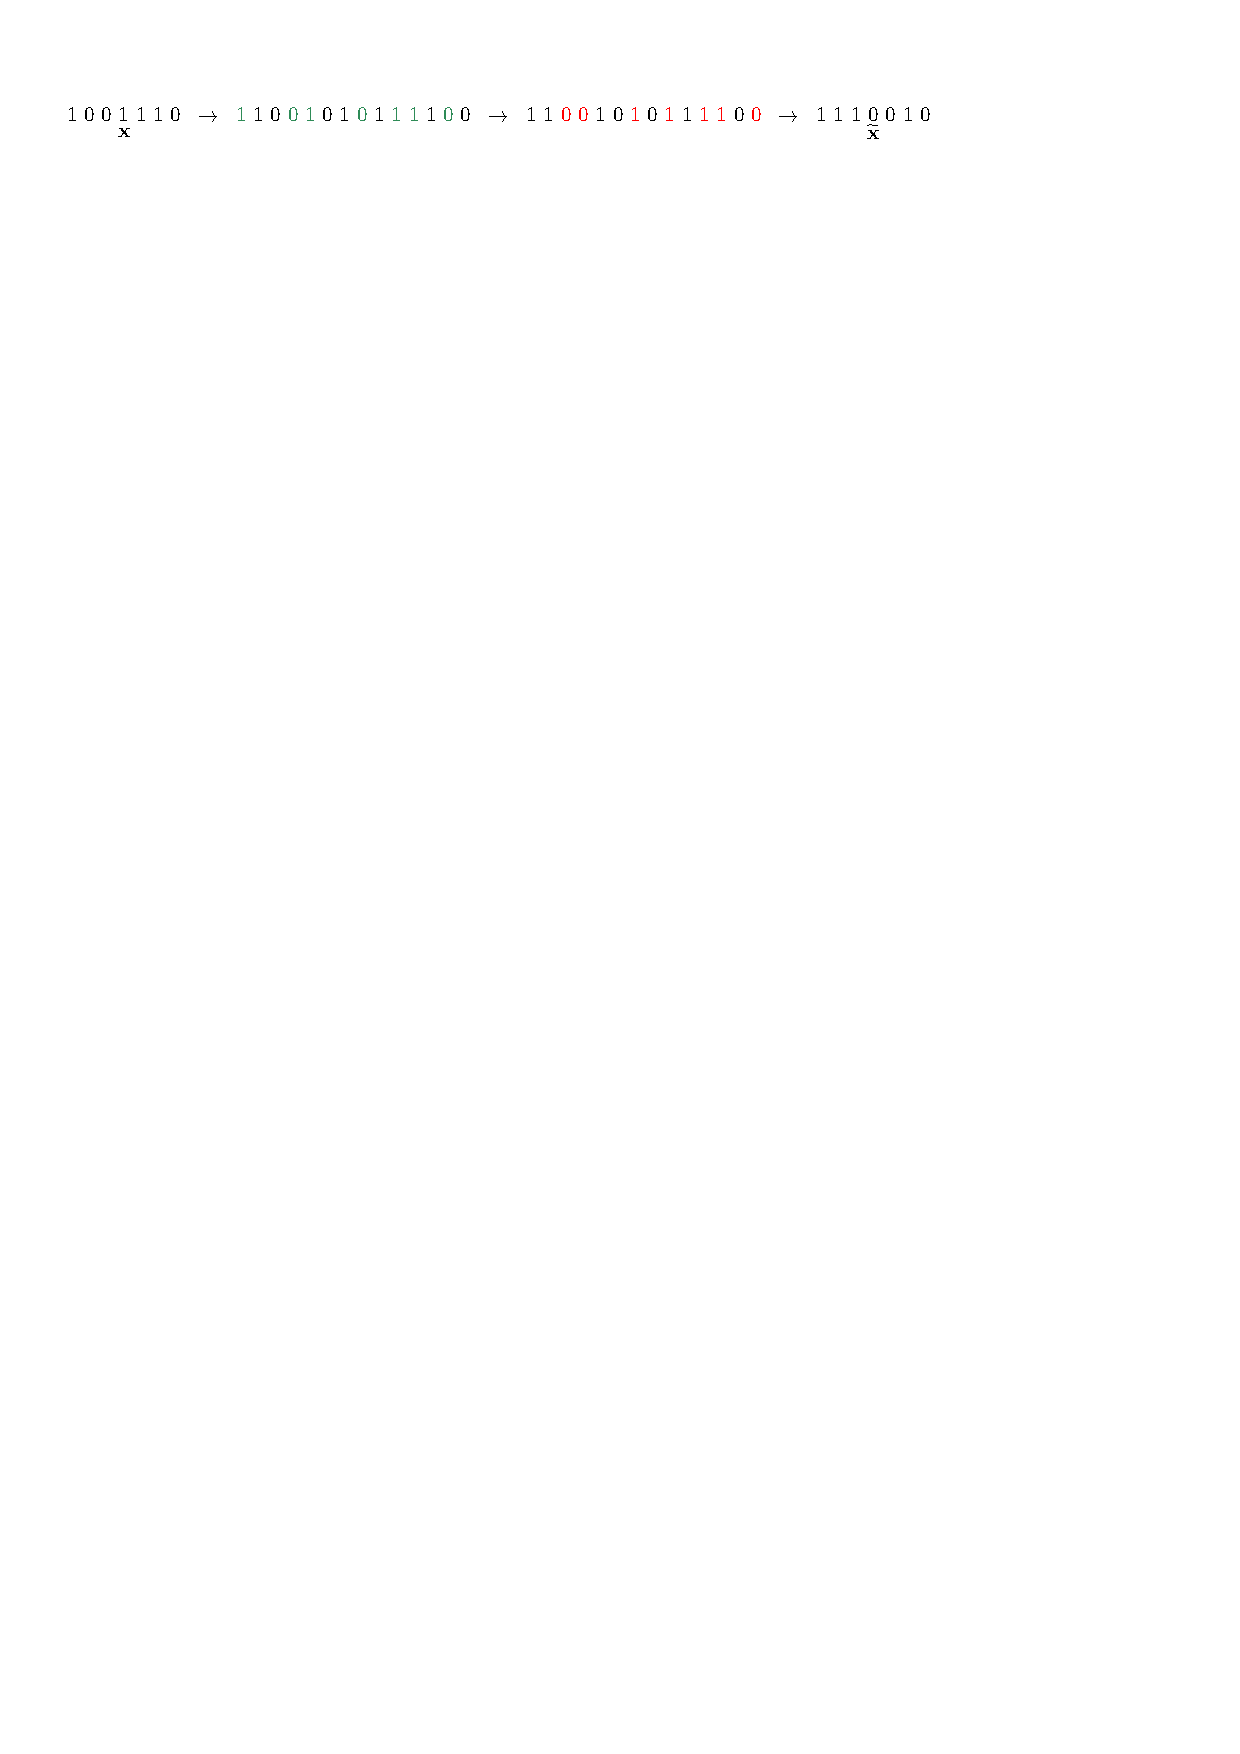
\includegraphics[scale=1]{insertion-deletion2}
	\caption{We obtain a trace $\xt$ by sending $\x$ through the deletion-insertion channel. Inserted bits are shown in green and deleted bits are shown in red.}
	\label{fig:trace}
\end{figure}


Suppose that the input string $\x$ is unknown. The {\bf trace reconstruction problem} asks
the following: How many i.i.d.\ copies of the trace $\xt$ do we
need in order to determine $\x$ with high probability? (See Section \ref{sec:reconstruction} and Appendix \ref{sec:proofmainthm} for more formal problem descriptions.)

There are two variants of this problem: the ``worst case'' and the ``average case'' (also referred to as the ``random case''). In the worst case variant, we want to obtain bounds which hold uniformly over all possible input strings $\x$. In the average case variant, the input string is chosen uniformly at random. In this paper, we study the average case.

\citet*{HMPW08} gave an algorithm for reconstructing random strings from the deletion channel using polynomially many traces, assuming the deletion probability $q$ is sufficiently small. \cite{PZ17} proved that $\exp(O( \log^{1/2}n ))$ many traces suffice for the deletion channel when the deletion probability $q$
is below $1/2$. Before the current work, the upper bound on the number of traces required for
$q \geq 1/2$ was the same as for worst case strings, i.e.,
$\exp(O( n^{1/3} ))$ (see works of \citet*{DOS16,NP16}).  We improve the
upper bound for all $q\in[0,1)$, and prove a result which
also holds when we allow insertions.  We remark that the trace reconstruction problem is significantly more difficult for $q>1/2$\footnote{Suppose that $q>1/2$, the string $\w$ is an arbitrary string of length $(1-q)n$, and $\x$ is a random string of length $n$. Then it holds with probability $1-\exp(-cn)$ that $\w$ is a subsequence of $\x$. To see this, observe that the number of bits in $\x$ until we see $w_0$ is a geometric random variable of mean 2. Iterating,  existence (with probability $1-\exp(-cn)$) of an appropriate subsequence holds by concentration for the sum of independent geometric random variables of mean 2. Therefore, by a union bound, if $q>1/2$, then any subexponential collection of strings of length $(1-q)n$ (typical for traces of the deletion channel) are, with high probability, all substrings of a random  string $\x$ of length $n$.} and that the alignment algorithm used by Peres and Zhai fails for the case of higher deletion probability.
\begin{theorem}\label{th:main}
	For $n\in\N$ let $\x\in\{0,1 \}^n$ be a bit string where the bits
	are chosen uniformly and independently at random.  Given $q,q'\in[0,1)$
	there exists $M>0$ such that for all $n$ we can reconstruct $\x$
	with probability $1-o_n(1)$ using $\lceil\exp(M\log^{1/3}n)\rceil$ traces
	from the deletion-insertion channel with parameters $q$ and $q'$.
\end{theorem}
%
We remark that the upper bound $\exp(O(\log^{1/3} n))$ in
the main theorem is the best one can obtain without also
improving the upper bound $\exp(O(n^{1/3}))$ for worst case strings.
This holds because, given an arbitrary string of length
$m = \log_{2+\eps} n$ for $\eps>0$, this string will appear
in a random length $n$ string with probability converging to 1 as
$n\rta\infty$.  In particular, a given worst case string of length $m$
is likely to appear in our random string, and the best known algorithm
for reconstructing this string requires $\exp(\Omega(m^{1/3}))
= \exp(\Omega(\log^{1/3} n))$ traces. See Lemma 10 in \cite{MPV14} for the details of this reduction.

 
We remark that our methods can be adapted easily to certain other
reconstruction problems, e.g., to the case where one allows substitutions
in addition to deletions and insertions, and the case where the bits
in the input $\x$ are independent Bernoulli($r$) random variables for arbitrary
$r\in(0,1)$, instead of $r=1/2$. We also note that there is a simple reduction (described, e.g., in \cite{MPV14} and \cite{DOS16})  of the trace reconstruction problem for larger alphabets to the case of bits. Moreover, as shown in \cite{MPV14},   trace reconstruction  becomes much easier if the alphabet size grows as $\Omega(\log n)$.


\section{Related work}

The trace reconstruction problem dates back to the early 2000's in works of \citet*{L01a,L01b,BKKM04}. Batu, Kannan, Khanna and McGregor, who were partially motivated by the study of mutations, considered the case where the deletion probability $q$ is decreasing in $n$. They proved that if the original string $\x$ is random and the deletion probability $q=O(1/\log n)$, then $\x$ can be constructed with high probability using $O(\log n)$ samples. Furthermore, they proved that if $q=O(n^{-(1/2+\eps)})$, then every string $\x$ can be reconstructed with high probability with $O(n\log n)$ samples.

\citet*{HMPW08} considered the case of random strings and constant deletion probability. They gave an algorithm for reconstruction with polynomially many traces when the deletion probability $q$ is less than some small threshold $c$. The threshold $c$ is not given explicitly in the work of \citet*{HMPW08}, but was estimated by \cite{PZ17} to be at most $0.07$.

The result of \cite{HMPW08} was improved by \cite{PZ17}. They showed that a subpolynomial number of traces $\exp(O(\log^{1/2} n))$ is sufficient for reconstruction, and they extended the range of allowed $q$ to the interval $[0,1/2)$. %YYY For $q<1/2$ a

Our work improves the above results in three ways. First, we improve the upper bound to  $\exp(O(\log^{1/3} n))$. Second, we allow for any deletion and insertion probabilities in $[0,1)$. Third, unlike \cite{PZ17}, our method works not only for the deletion channel, but also for the case where we allow insertions and substitutions.

It is shown by \cite{HMPW08} that $\exp(O(n^{1/2} \log n))$ traces suffice for reconstruction with high probability with worst case input. This was  improved to $\exp(O(n^{1/3}))$ independently by \citet*{DOS16} and by \citet*{NP16}. Until the current work, the average case upper bound was equal to the worst case upper bound for $q\geq 1/2$. The techniques developed by \cite{DOS16,NP16} are applied in the current work and the work of  \cite{PZ17} to certain shorter substrings of our random string.

The best lower bounds for the number of required traces are  $\Omega(\log^2 n)$
\citet*{MPV14}) in the average case and
$\Omega(n)$ in the worst case (\citet*{BKKM04}). Trace reconstruction for the setting which allows insertions and substitution in addition to deletions was considered by \citet*{KM05}, \citet*{VS08}, \citet*{DOS16}, and \citet*{NP16}. We refer to the introduction of the paper by \citet*{DOS16} and the survey of \citet*{M09} for further background on the deletion channel.


\section{Construction of the channel}
\label{sec:reconstruction}

To simplify notation we will consider bit strings of infinite length
(rather than length $n\in\{1,2,\dots \}$) throughout the paper. Observe that if we can reconstruct the first $n$ bits of an infinite string, then we can also reconstruct length $n$ strings.
Let $\N=\{0,1,\dots \}$ and let $\cS := \{ 0 , 1 \}^\N$ denote
the space of infinite sequences of zeros and ones.   We denote
elements of $\cS$ by $\x := (x_0 , x_1 , \ldots)$.

Fix a deletion probability $q$ and an insertion probability $q'$ in $[0,1)$,
and let $p=1-q$ and $p'=1-q'$.
We construct $\xt$ from $\x$ by the
procedure described above, i.e., first, for each $j\in\N$ we insert $G_j-1$ uniform and independent bits before the $j$th bit of $\x$. The geometric random variables $G_j$ are independent and satisfy
\eqbn
\P[ G_j=v ]=(q')^{v-1}(1- q'),\qquad\forall v\in\{1,2,\dots \}.
\eqen
Then we delete each bit of the resulting string independently with probability $q$.

Let $\mu$ be the law of i.i.d.\ Bernoulli random variables with parameter $1/2$.
We denote $\P_\x := \P_{\delta_\x}$ the law of $\xt$ when $\x$ is fixed; write   $\P := \P_\mu$ for the law of $\xt$ when $\x$ is picked according to $\mu$,

We call the string $\xt$ a trace.  An example is
given in Figure~\ref{fig:fg}.

\begin{figure}[ht!]
	\centering
	\framebox{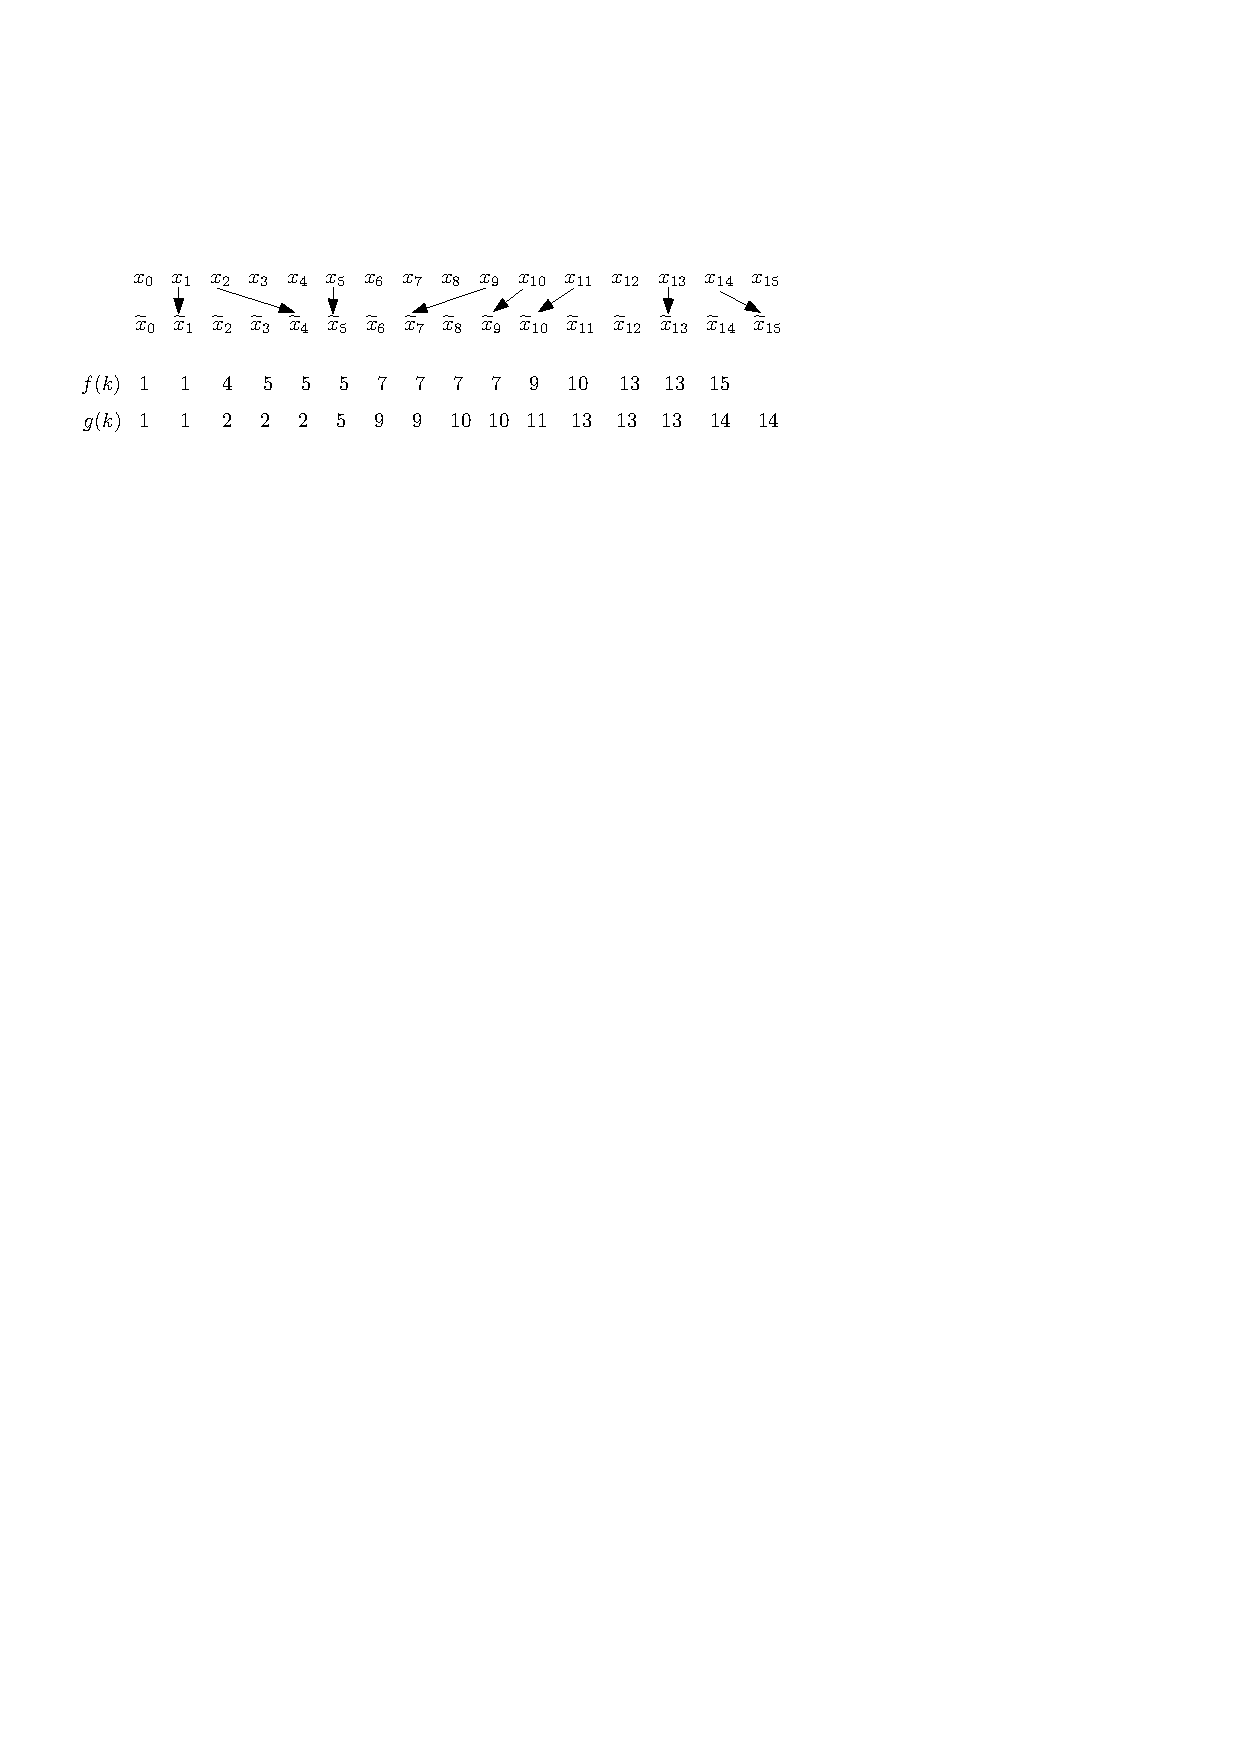
\includegraphics[scale=1]{fg}}
	\caption{Illustration of the functions $f$ and $g$.
		The arrows indicate bits which are copied from $\x$ to $\xt$.}
	\label{fig:fg}
\end{figure}

For $\x \in \cS$ and
$0 \leq i \leq j < \infty$ let $\x(i:j) \in \{ 0 , 1 \}^{j-i+1}$
denote the subsequence of $\x$ from position $i$ to $j$.
Let $\x(i:\infty)\in\{0,1\}^\N$ denote the substring of $\x$
corresponding to the bits in position $i$ or later.  Define $f$
such that $f(k)$ is the location in $\xt$ of the first bit of
$\x(k:\infty)$ that is preserved by the channel.  Let $g$ be
the approximate inverse of $f$, defined such that $g(k')$ is
the location in $\x$ of the first bit of $\xt(k':\infty)$ which
was copied from $\x$. Observe that $g(f(k))=k$ if and only if
bit $k$ of $\x$ was copied to $\xt$.

If $\x\in\{0,1 \}^n$ is a string of finite length, then we construct the trace $\wt\x$ similarly: Let $q\in[0,1)$ be the deletion probability and let $q'\in[0,1)$ be the insertion probability. First, for each $j$, before the $j$th bit of $\x$ we insert $G_j-1$ uniform and independent bits, where the independent geometric random variables $G_j\ge 1 $ have parameter $1-q'$. Then we delete each bit of the resulting string independently with probability $q$.



\subsubsection*{Worst case reconstruction problem}
Let $q,q'\in[0,1)$. For any $N\in\N$ let $\P_{\x}^{N}$ denote the probability measure associated with $N$ independent outputs of the deletion-insertion channel $\P_{\x}$ with deletion (resp.\ insertion) probability $q$ (resp.\ $q'$).  For $n\in\N$
and $\x\in\{0,1 \}^n$ let $\frk X$ denote a
collection of $N_n\in\N$ traces sampled independently at random.
We say that worst case strings of
length $n$ can be reconstructed with probability $1 - o_n(1)$
from $N_n$ traces, if there is a function $G\colon  \cS  ^{N_n} \to \{0,1 \}^n$, such that for all $\x\in\cS$,
\eqbn
\P_{\x}^{N_n}[G(\mathfrak X ) = \x(0:n-1)] = 1-o_n(1).
\eqen

\subsubsection*{Average case reconstruction problem}

Let $\mu_n$ denote uniform measure on $\{0,1 \}^n$.  We say that uniformly random strings of length $n$
can be reconstructed with probability $1-o_n(1)$ from $N_n$ traces
if we can find a set $\cS_n\subset\{0,1 \}^n$ with $\mu_n(\cS_n)=1-o_n(1)$, and a function
$G\colon  \cS^{N_n} \to \{0,1 \}^n$,
such that for all
$\x\in\cS$ for which $\x(0:n-1) \in\cS_n$, we have
\eqbn
\P_{\x}^{N_n}[G(\mathfrak X ) = \x(0:n-1)] = 1-o_n(1).
\eqen
%
In particular, Theorem \ref{th:main} says that uniformly random strings
can be reconstructed from $N_n := \lceil\exp(M\log^{1/3}n)\rceil$ traces with probability $1-o_n(1)$.



\section{Outline of proof} \label{ss:outline}

We reconstruct the bits of $\x$ one by one.  For any $k,n \in \N$ with
$k <n$ we assume $\x(0:k)$ is given, and we show that with
probability $1-O(n^{-2})$ we can use $\lceil\exp(M\log^{1/3}n)\rceil$
traces to determine the subsequent bit $x_{k+1}$. Furthermore, we show that the traces can be reused in each step, so the same set of traces can be used to reconstruct the $k$th bit and the $k+1$st bit. When $\x$ is
chosen from $\mu$ and the traces are then generated i.i.d.\ from $\P_\x$, the algorithm will fail at step $k$ with probability
$O(n^{-2})$, producing an incorrect guess or no guess at all.
Inductively, we see that the probability after $k+1$ steps that the
algorithm has failed to correctly identify $\x(0:k)$ is $O(k n^{-2})$;
setting $k=n$, the probability of not correctly identifying $\x(0:(n-1))$
is $O(n^{-1})$, as desired.  For most of the paper we assume, in order to simplify notation, that $q = q'$.
We explain at the end of Appendix \ref{sec:proofmainthm} how to treat the case of general $q,q'$. 

Three ingredients are required, as follows.
\begin{enumerate}[$(i)$]
	\item  A Boolean test $T(\w, \wt\w)$ on pairs $(\w, \wt\w)$ of bit strings	of finite equal length, indicating whether $\wt\w$ is a plausible match for the string $\w$ sent through the deletion-insertion channel.
	\item An alignment procedure that uses the test $T$ repeatedly to
	produce for each of the independent traces $\xt$ an estimate $\tau$
	for a carefully chosen position $f(k_*)$ in $\xt$ nearby $f(k)$.
	\item A bit recovery procedure based on a method of~\citet*{PZ17,DOS16,NP16} to produce
	from the approximately aligned traces an estimate of the subsequent bit
	or bits.
\end{enumerate}

The argument of \citet*{PZ17} follows the same overall structure, with an alignment step followed by a reconstruction step for each bit in the original string. However, the greedy alignment step of \citet*{PZ17} relies crucially on the  assumption that the deletion probability $q<1/2$, and that no insertions are allowed. We overcome this problem by introducing a new kind of test for the alignment, which is based on studying correlations between blocks in the input string and in the trace.

We end the introduction by providing more details on the ingredients
$(i)-(iii)$ above (in a slightly different order: $(ii)$, $(i)$, $(iii)$).
Appendix \ref{sec:proofmainthm} contains a proof of the main theorem
modulo two key results, Theorems ~\ref{th:align} and~\ref{th:complex} below. Appendix~\ref{sec:test2} constructs
the test $T$. Appendix~\ref{sec:find} uses this to construct
a good position $k_*$ in the input to try to align.
Appendix~\ref{sec:align} constructs an approximate alignment
$\tau_1$ and a good alignment $\tau_2$, and establishes
properties of these culminating in one of the two key results (Theorem~\ref{th:align}).  Finally, Appendix~\ref{sec:recover}
finishes the proof of the main theorem by proving the other key
result (Theorem~\ref{th:complex}).

\subsubsection*{Alignment: Finding $f(k_*)$ in the trace}
The following is our key alignment result. Assume $\x(0:k)$ is known for some $k\in\N$. We find a position $k_*<k$ satisfying $|k-k_*|=\Theta(\log n)$, and we have an algorithm which finds an estimate $\tau_2$ for $f(k_*)$ in the trace $\wt\x$. For all $\x$ outside some exceptional set $\bad$, the theorem gives
a lower bound for the probability of true positives (meaning $|f(k_*)-\tau_2|\leq \calign\log^{1/3} n$, with $\calign$ as below),
an upper bound for the probability of false positives (meaning $|f(k_*)-\tau_2|> \calign\log^{1/3} n$), and
an upper bound for the average discrepancy in the case of true positives. We give a brief outline of the alignment algorithm mentioned in the following theorem right below the statement of the theorem.
\begin{theorem}[proved in Appendix~\ref{sec:align}] \label{th:align}
	Given any $\csep>0$ there are constants $\cback, \calign, \cfalse, \ctrue, \cavg \geq 1$ such that the following hold for any fixed an integer $k \in [2 \cback \log n ,  n]$, where we let $k_*$ and $\tau_2$
	be the message\footnote{By ``message'' we mean the input string.} position and alignment pointer, respectively, produced
	by the alignment algorithm in Appendix~\ref{sec:align} when the algorithm
	assumes correctly the value of $\x(0:k)$.
	\begin{enumerate}[$(i)$]
		\item $\tau_2$ is bounded above by $2n$ when finite and (given $\x(0:k)$), is
		a stopping time on the filtration determined by $\xt$, i.e., for each $i$,
		$$\mbox{the event } \{ \tau_2 \leq i \} \mbox{ is a function of }
		\wt\x(0:i) \mbox{ and } \x(0:k).$$
		\label{r:i}
	\end{enumerate}
	\vspace{-25pt}
	Furthermore, there is a set $\bad$, determined by the first
	$2n$ bits of $\x$, such that $\mu(\bad) = O(n^{-2})$ and if
	$\x \notin \bad$, then the following four properties hold for
	sufficiently large $n$.
	\begin{enumerate}[$(i)$] \setcounter{enumi}{1}
		\item $k_*$ is order $\log n$ from the end of the reconstructed input:
		$$k - \cback \log n \leq k_* \leq k - \frac{\cback}{2} \log n.$$
		\label{r:ii}
		\item The true positive rate is not too tiny:
		$$\P_\x \left [ |g(\tau_2) - k_*| \leq \calign \log^{1/3} n \right ]
		\geq \exp (-\ctrue \log^{1/3} n ).$$
		\label{r:iii}
		\item The false positive rate is much smaller than the true positive rate:
		$$\P_\x \left [ \infty > |g(\tau_2) - k_*| > \calign \log^{1/3} n \right ]
		\leq \exp(- \cfalse \log^{1/3} n).$$
		with $\cfalse - \ctrue > \kappa := \csep ( 8 \cavg + \cback^{1/3} )$.
		\label{r:iv}
		\item The average discrepancy when there is a true positive test
		is at most a small constant multiple of the threshold:
		$$\E_{\x} \left [ |g(\tau_2) - k_*|
		\1_{|g(\tau_2) - k_*| \leq \calign \log^{1/3} n} \, \big{|} \,
		\tau_2 < \infty \right ] \leq \cavg \log^{1/3} n.$$
		\label{r:v}
	\end{enumerate}
\end{theorem}
In our proof of the theorem, we find our estimate $\tau_2$ for $f(k_*)$ in two steps. In the first step we tolerate that our initial estimate $\tau_1$ has error $O(\log n)$, and in the second step we tolerate that our estimate $\tau_2$ has error $O(\log^{1/3}n)$. Both steps are based on defining a function $T$ which takes as input two substrings $\w$ and $\wt\w$ (from the string and from the trace, respectively) of the same length $\ell\in\N$, and returns the value 1 (resp.\ 0) if it seems likely (resp.\ unlikely) that $\wt\w$ was obtained by sending $\w$ through the deletion-insertion channel. Each string $\w$ and $\wt\w$ can be viewed as a length $\ell$ random walk by looking at the partial sums (where 1 gives an increment of $+1$ and $0$ gives an increment of $-1$), and our test is based on comparing the increments of these two walks in certain subintervals (see details below).

In this paragraph we outline the method we use for $k$ at least a large constant multiple of $\log^{5/3} n$ (the alignment is generally easier for smaller $k$). %Assume $k$ is at least a large constant multiple of $\log^{5/3} n$.
In the first step we let $\w_1$ be a substring of length $\ell_1=O(\log^{5/3} n)$ in $\x$, such that the right end-point $k_0$ of $\w_1$ satisfies $k_0<k$ and $|k-k_0|=\Theta(\log n)$. For each trace we evaluate $T(\w_1,\wt\w)$ for each length $\ell_1$ substring $\wt\w$ of $\xt$, going from left to right in $\xt$. Our estimate $\tau_1$ for $f(k_0)$ is the right end-point of the first substring $\wt\w$ for which $T(\w_1,\wt\w)=1$. If we find no such substring $\wt\w$ in $\xt(0:2k_0)$, then we set $\tau_1=\infty$, and we do not use this trace when we estimate $x_{k+1}$. We say that we have a true (resp.\ false) positive if $\tau_1<\infty$, and if $|\tau_1-f(k_0)|$ is smaller (resp.\ larger) than a constant multiple of $\log n$. We prove that, except for $\x\in\bad$, the probability of true and false positives satisfy similar bounds as in $(iii)$ and $(iv)$ of Theorem \ref{th:align} (but with other constants than $\ctrue$ and $\cfalse$).

In the second step we let $\w_2$ be a substring of length $\ell_2=O(\log^{1/3} n)$ in $\x$, such that the right end-point $k_*$ of $\w_2$ satisfies $k_0<k_*<k$ and $|k-k_*|,|k_0-k_*|=O(\log n)$. As above, we go through a substring of $\xt$ from left to right, and we let $\tau_2$ be the right end-point of the first substring $\wt\w$ of length $\ell_2$ for which $T(\w_2,\wt\w)=1$. Using the estimate $\tau_1$ to $f(k_0)$ from the first step, it is sufficient to only search through a substring of length $O(\log n)$ near $\tau_1$.

\begin{figure}
	\centering
	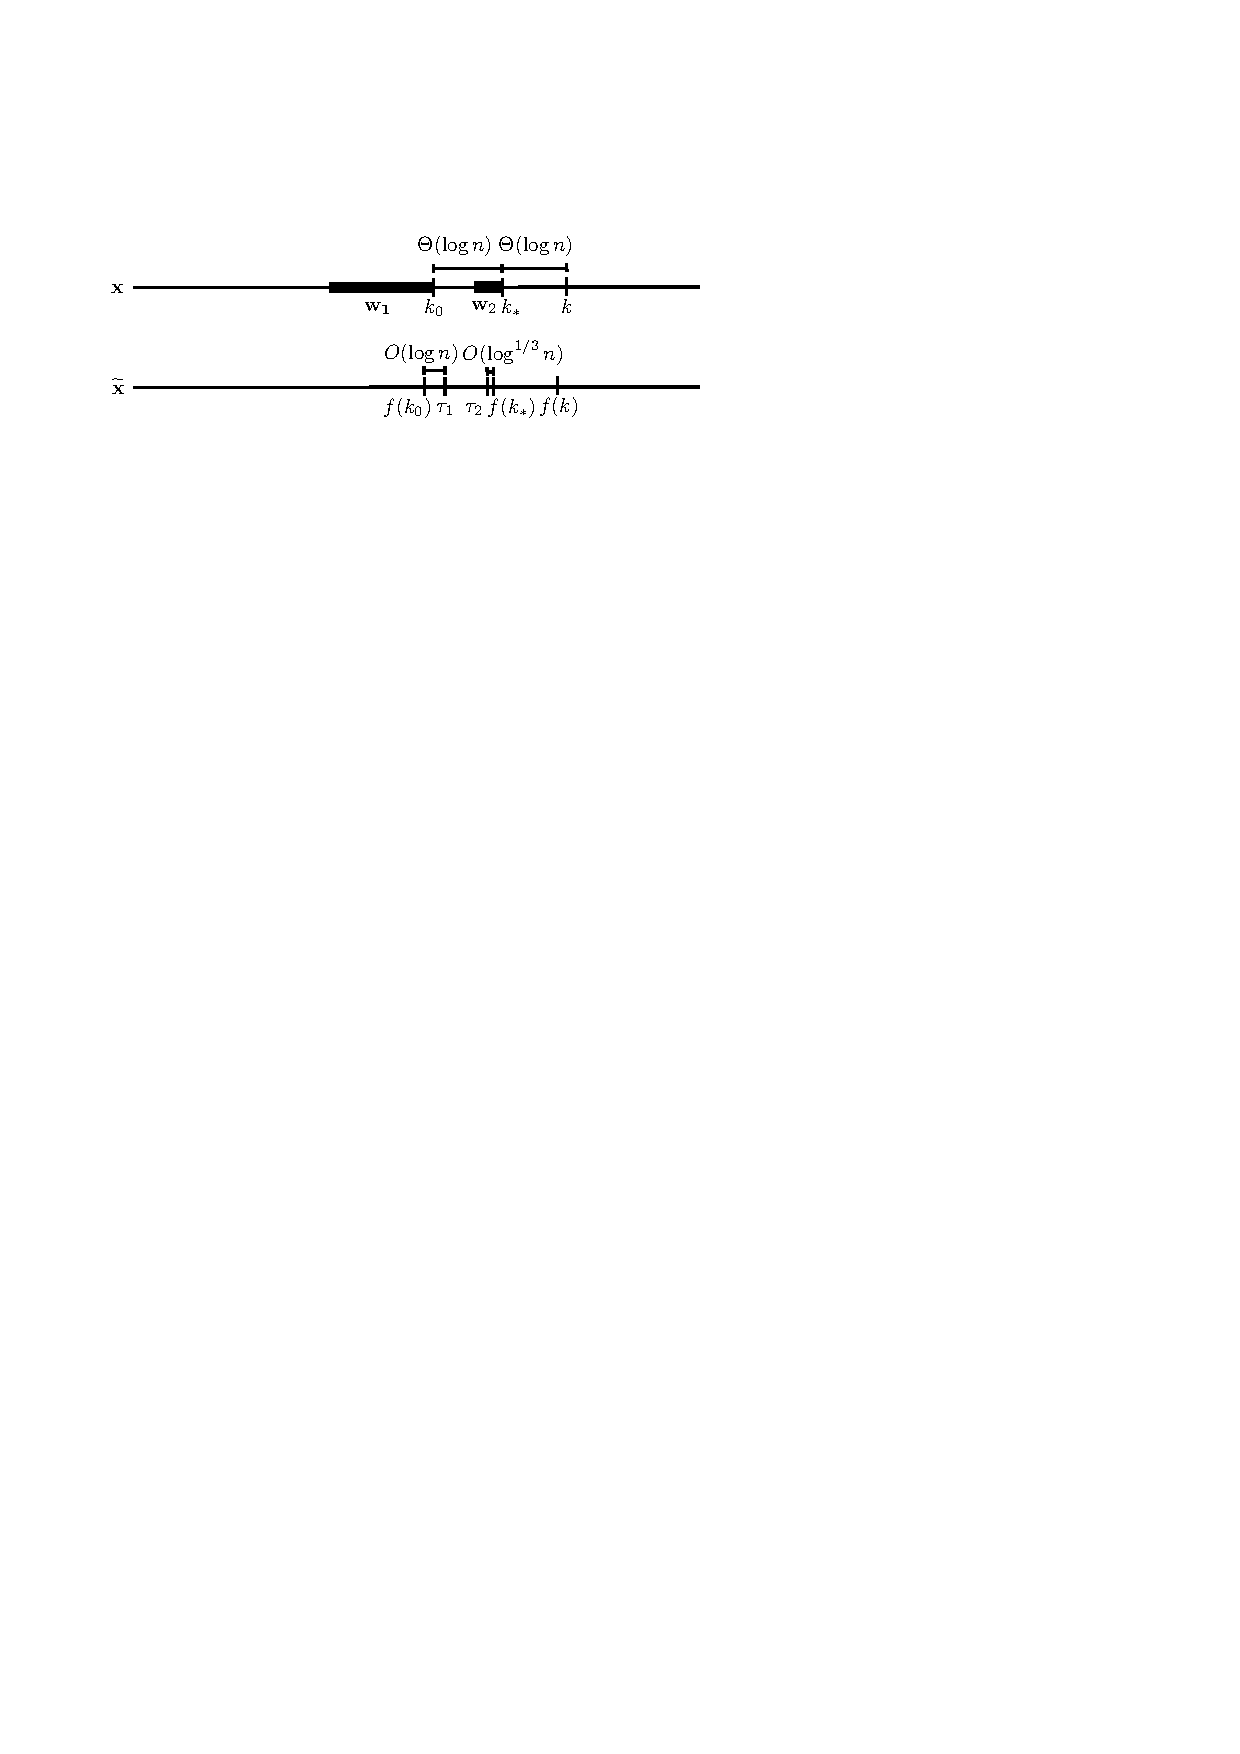
\includegraphics[scale=1]{alignment-outline}
	\caption{Illustration of indices considered in our two alignment steps. In the first alignment step we find an approximation $\tau_1$ to $f(k_0)$, and in the second alignment step we find an approximation $\tau_2$ to $f(k_*)$.}
\end{figure}

Since we are using a shorter substring to align than in the first step, the test is less robust. For example, there may be several substrings $\w_2$ and $\wh\w_2$ in the input string which are close to each other (distance $O(\log n)$) and similar in the sense that the associated walks have similar increments. If this is the case, we risk consistently choosing $\tau_2$ such that $g(\tau_2)$ is near the right end-point of $\wh \w_2$ instead of the right end-point of $\w_2$. In order to avoid this, we choose $\w_2$ carefully, such that there are no other nearby substrings $\wh\w_2$ with this property.


\subsubsection*{The test}
We will describe a simplified version of the test $T$. Given strings $\w$ and $\wt\w$ of the same length $\ell\in\N$ and some $\lambda\in\{1,\dots,\lfloor \ell^{1/2} \rfloor \}$, divide each string $\w$ and $\wt\w$ into $\lceil\ell/\lambda \rceil$ blocks of length approximately $\lambda$. For $i=1,\dots,\lceil\ell/\lambda\rceil$ let $s_i$ (resp.\ $\wt s_i$) denote the sum of
$(2x_j - 1)$ as $j$ ranges over positions in the $i$th block of
$\w$ (resp.\ $\wt\w$), and we enumerate the blocks from left to right.
Observe that $s_i$ and $\wt s_i$ both have expectation 0, and that $s_i>0$
(resp.\ $\wt s_i>0$) exactly when more than half of the bits in the $i$th
block of the string (resp.\ trace) are equal to 1. For some appropriately chosen $c_1\in(0,1)$ define
\eqb
T(\w,\wt\w) =
\begin{cases}
	1\qquad \displaystyle \text{\,\,if\,\,\,}\sum_{i=1}^{\lceil\ell/\lambda\rceil} \op{sign}(s_i)\cdot\op{sign}(\wt s_i) >  c_1 \ell/\lambda,\\
	0\qquad\text{otherwise}.
\end{cases}
\label{eq15}
\eqe
Observe that if $\w$ and $\wt\w$ are sampled independently and uniformly from $\{0,1 \}^\ell$, then $T(\w,\wt\w)=0$ except on an event of probability $\exp(-\Theta(\ell/\lambda ))$. On the other hand, if $\wt\w$ was obtained by sending $\w$ through the deletion-insertion channel, one can show that with probability $\exp(-\Theta(\ell/\lambda^2 ))$, for most blocks $i$ a constant fraction of the bits in the trace were copied from the corresponding block in the input string. On this event, by choosing $c_1$ sufficiently small, we have $T(\w,\wt\w)=1$ with uniformly positive probability. We will deduce from this that the probability of a false positive is $\exp(-\Omega(\ell/\lambda))$, while the probability of a true positive is $\exp(-O(\ell/\lambda^2 ))$. In the first alignment step we use the test with $(\ell,\lambda)$ of order $(\log^{5/3}n,\log^{2/3}n)$, and in the second alignment step we use the test with $(\ell,\lambda)$ of order $(\log^{1/3}n,1)$.

\begin{figure}[ht]
	\centering
	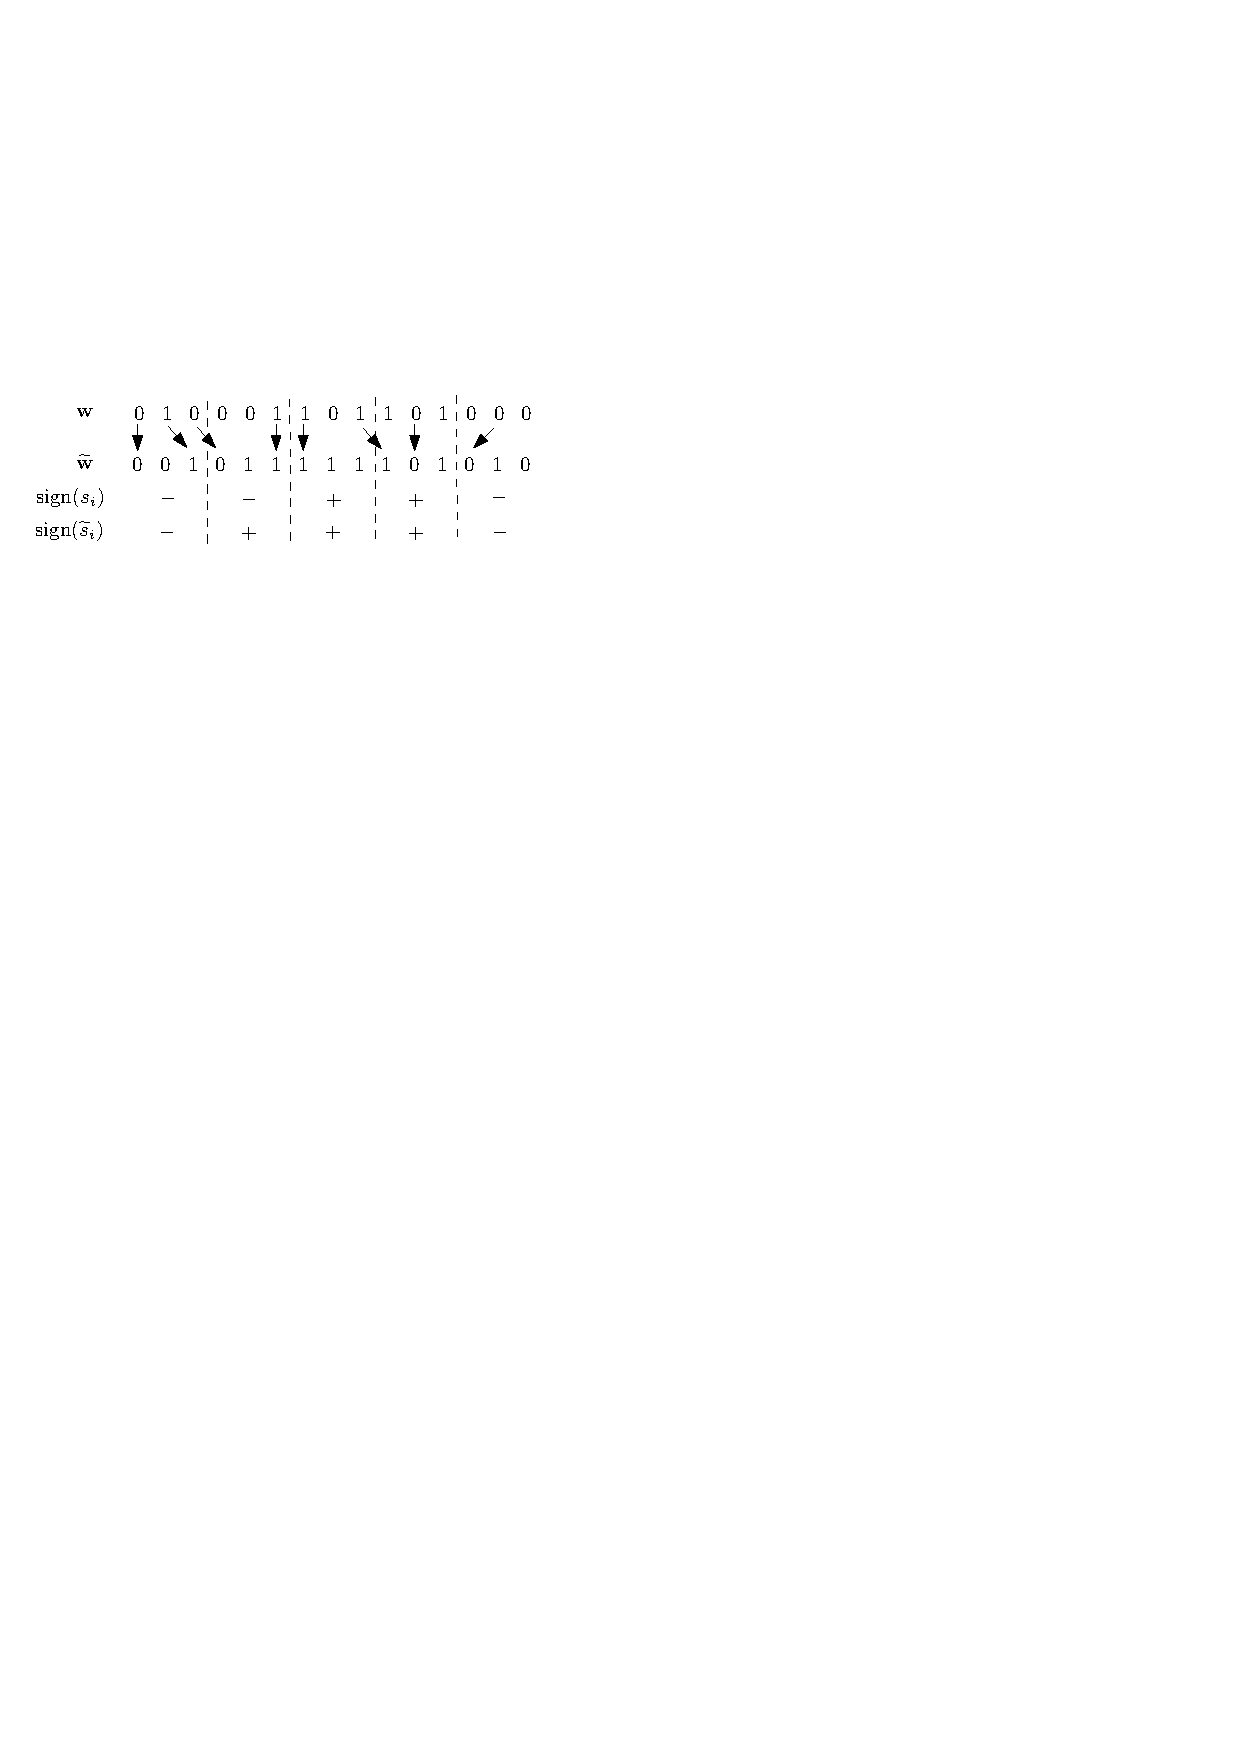
\includegraphics[scale=1]{test}
	\caption{Illustration of our test $T$. We divide the length $\ell=15$ substrings $\w$ and $\wt{\w}$ of $\x$ and $\xt$, respectively, into blocks of length $\lambda=3$, and find the sign of the sum of the bits in each block (replacing 0 by $-1$). If many bits in block $i$ of $\xt$ were copied from the corresponding block of $\x$, then the sums in block $i$ are positively correlated, and their signs are the same with probability strictly larger than $1/2$. Our test $T$ counts how many blocks for which the signs match, and use this to predict whether the right end-points of the two substrings are likely to correspond to each other as described by the functions $f$ and $g$.
	}
\end{figure}

The actual function $T$ we use differs from this simplified test in two ways: First,  we need to prove $(v)$ of Theorem \ref{th:align}, with $\cavg$ sufficiently small as compared to the other constants, in order for our reconstruction algorithm to work. For the test described above it is not clear that this holds, due to the effect described in Figure \ref{fig2}. To resolve this, we define a second test similarly as in \eqref{eq15}, but where, for some $0<c\ll 1$, we use $\w( (\ell-c\ell):\ell )$ and $\wt\w( (\ell-c\ell):\ell )$ instead of $\w$ and $\wt\w$. We require that both tests are positive when defining $\tau_2$. The first test, which uses the full strings $\w$ and $\wt\w$, ensures that the test gives false positives with very small probability, while the second test, which uses the shorter substrings, ensures that the constant $\cavg$ above is sufficiently small. The second way in which our test differs from the simplified test above, is that we choose to not sum over all the blocks $i=1,\dots,\lceil\ell/\lambda\rceil$ when defining $T$. Instead, we choose some $\theta\in(0,1)$ and use only the $\lfloor \theta\ell/\lambda \rfloor$ blocks for which $|s_i|$ is largest. This simplifies the proof of our lower bound for the probability of having true positives.

Consider the setting of the second alignment step above, where we evaluate $T(\w_2,\wt\w)$ for all $\wt\w$ in a certain interval and $k_*$ is the right end-point of $\w_2$. With the above test, there are three sources of false positives.
First, as described above, $\w_2$ might be similar to some nearby substring $\wh\w_2$ of $\x$, such that we often get a positive test when considering the part of the trace corresponding to $\wh\w_2$.
Second, we could have unusually many deletions or insertions right before $f(k_*)$, which could make bits in the $i$th block of $\wt\w$ be copied from the $i$th block of $\w_2$, even if the right end-point of $\wt\w$ is far from $f(k_*)$ (see Figure \ref{fig2}).
Third, even if none of the above scenarios occur, there is a small chance that $T(\w_2,\wt\w)=1$, due to the randomness of the deletions and insertions. By choosing $\w_2$ appropriately, we can ensure that only the two latter sources of error are relevant. Then the errors are mainly caused by the randomness of the deletions and insertions, and not the randomness of $\x$, so the errors happen approximately independently for each trace. Both errors have probability $\exp(-\Omega(\log^{1/3}n))$ with the parameter values used above.

\begin{figure}
	\centering
	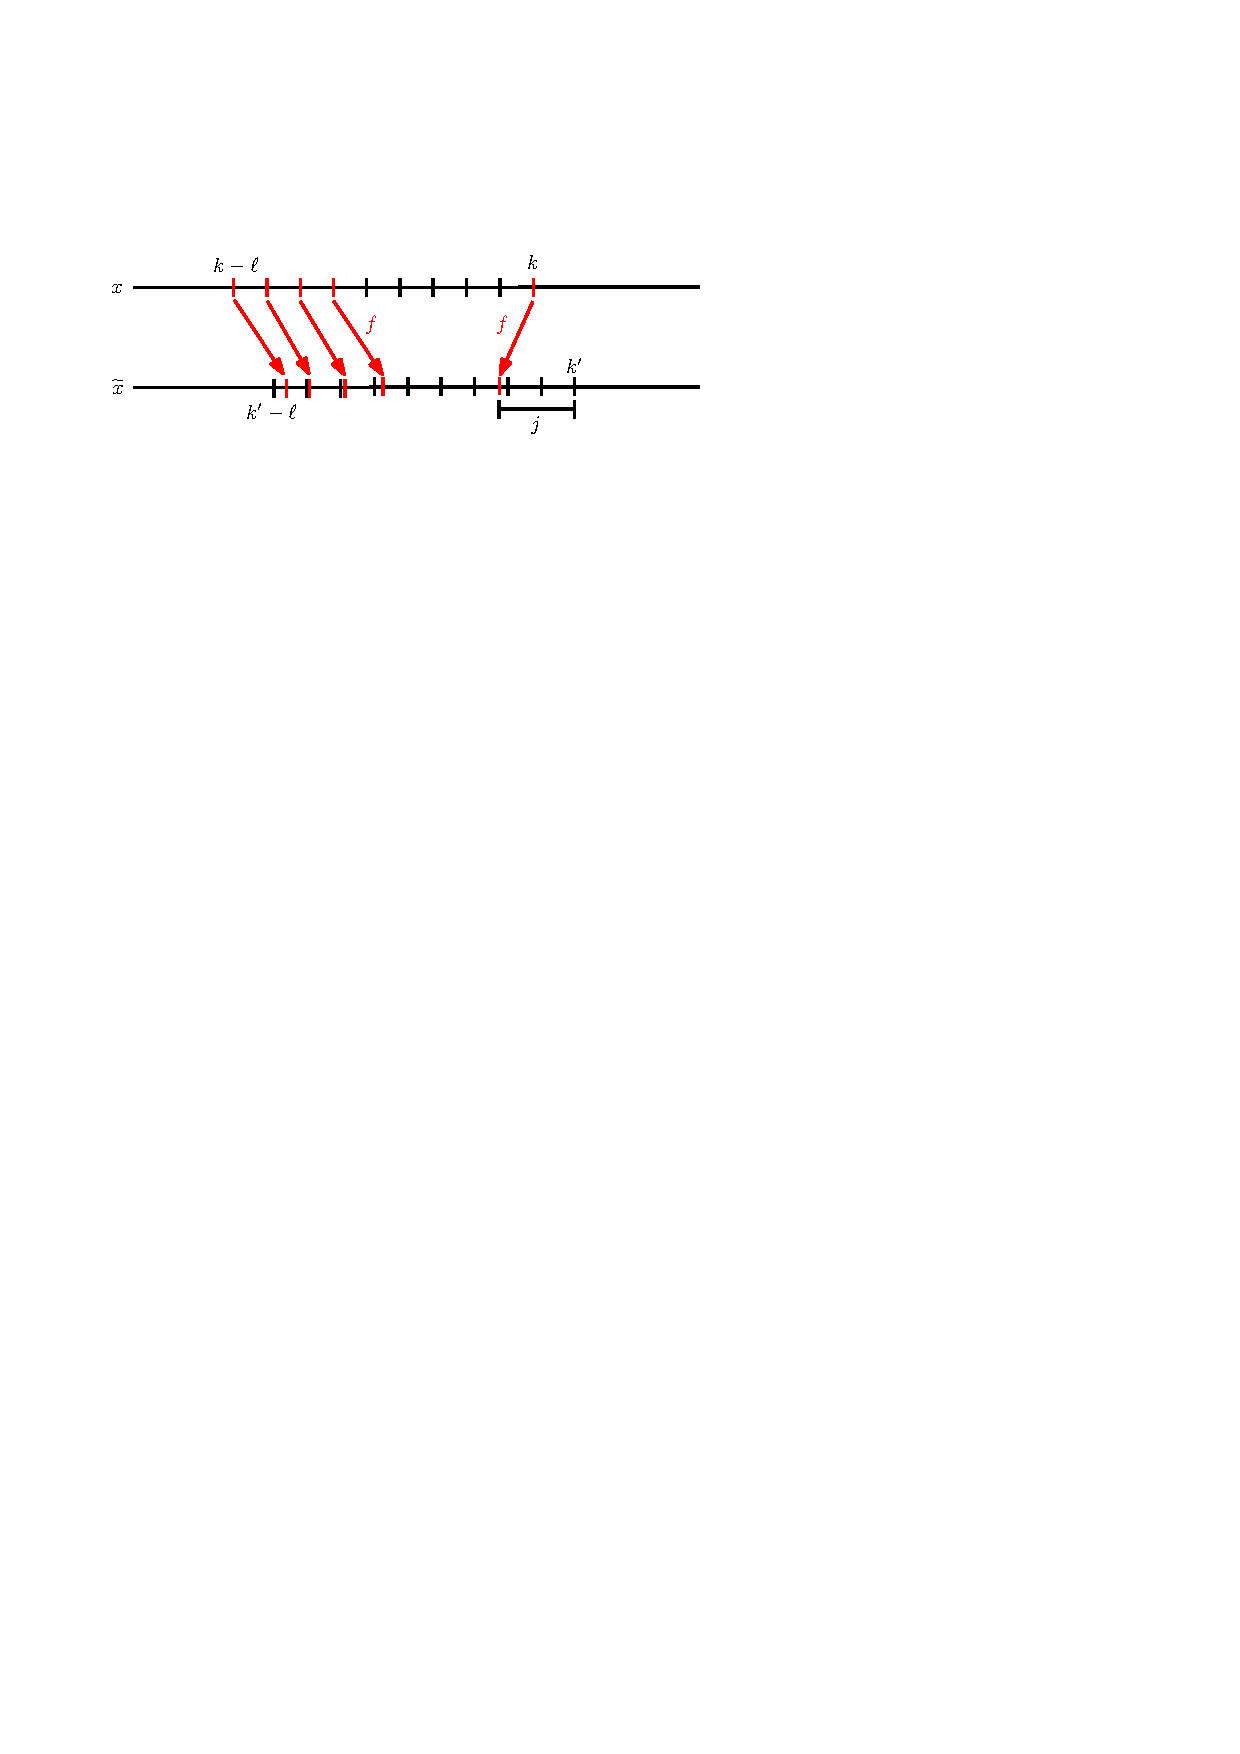
\includegraphics[scale=1]{overlap}
	\caption{The red arrows to the left indicate that bits in first few blocks of $\x$ are copied to the corresponding blocks of $\xt$. If this happens for many blocks, the test $T$ is likely to be positive, even if $j:=k'-f(k)$ is large. }
	\label{fig2}
\end{figure}



\subsubsection*{From alignment to reconstruction}
Finally, we explain how we can use our estimate $\tau_2$ for $f(k_*)$ in each trace to determine $x_{k+1}$. \cite{DOS16,NP16} proved that strings of length $m$ can be reconstructed with $\lceil\exp(O(m^{1/3}))\rceil$ traces by using single bit statistics for the traces. We prove the following variant of this result (following \cite{PZ17}) for the case where the input string has been randomly shifted before being sent through the deletion-insertion channel. The theorem implies that for different input strings $\x^{(1)}$ and $\x^{(2)}$ there exists some $j$, such that we can distinguish between the two strings by studying the average of the $j$th bit for the $\lceil\exp(M\log^{1/3}n)\rceil$ traces.

\begin{theorem}[proved in Appendix~\ref{sec:recover}]
	\label{th:complex}
	There are positive constants $\csep$ and $\cfwd$ depending only on
	$q$ and $q'$, not on $m$, $d$ or $\sigma$ below, such that the
	following separation criterion holds.
	Let $d$ and $m$ satisfy $d \leq m^{2/3}$ and let $\x^{(1)}$
	and $\x^{(2)}$ be any two infinite strings of bits such that
	$\x^{(1)} (0:d) = \x^{(2)}(0:d)$ but $\x^{(1)} (0:m) \neq \x^{(2)}(0:m)$.
	Let $\theta^s$ denote the shift by $s$ on infinite bit strings and
	for $i = 1,2$ and $j \geq 0$ let $q_{s,j}^{(i)} := \P_{\theta^s \x^{(i)}}
	[\wt x_j = 1]$ be the probability of a~1 in position~$j$ when $\x^{(i)}$ is
	shifted by $s$ and then run through the deletion-insertion channel.
	Let $\sigma$ be any probability measure on $\{ 0 , \ldots , d \}$
	with expected absolute deviation from its mean $\gamma$ satisfying
	$\sum_{s=0}^d \sigma (s) |s - \gamma| \leq m^{1/3}$.  Denote the averages
	of $q^{(i)}_{s,j}$ under $s \sim \sigma$ by
	$$q_{\sigma , j}^{(i)} := \sum_{s=0}^d \sigma (s) q_{s,j}^{(i)} \, .$$
	%
	Then there is some $j = j(\x^{(1)}, \x^{(2)}, m, d, \sigma) < \cfwd m$,
	such that
	%
	\eqb \label{eq:sep0}
	\left | q_{\sigma , j}^{(1)} - q_{\sigma , j}^{(2)} \right |
	\geq \exp (- \csep m^{1/3}) \, .
	\eqe
\end{theorem}
The proof uses complex analysis techniques similar to those of \cite{DOS16,NP16,PZ17}. We first derive an exact formula where the bit statistics are expressed as the coefficients of a particular polynomial. Then we deduce the theorem by applying a result of \citet*{BE97}, which says that the modulus of certain polynomials cannot be too small everywhere on a small boundary arc of the unit disk.

Applying Theorem \ref{th:complex} with $m=O(\log n)$ allows us to determine $x_{k+1}$, using our estimate $\tau_2$ to $f(k_*)$. We apply the theorem repeatedly with all possible pairs of strings $\x^{(1)}$ and $\x^{(2)}$, such that the initial part of the strings are given by $\x(k_*:k)$, and we consider the traces $\wt\x(\tau_2+\lfloor\log^{4/9}n\rfloor:\infty)$. Using the alignment result of Theorem \ref{th:align} we can show that the random shift satisfies the assumptions of Theorem \ref{th:complex} with high probability. If one of the strings $\x^{(i)}$ is equal to our input string $\x$, then we can use \eqref{eq:sep0} to determine from our $\lceil\exp(M\log^{1/3}n)\rceil$ traces which of the two input strings is correct. It is sufficient to consider finitely many candidate strings $\x^{(1)}$ and $\x^{(2)}$, since strings which differ only for bits very far out are unlikely to affect the part of the trace we consider.

\bibliography{ref}
\appendix

\section{Proof of main theorem modulo two key results}
\label{sec:proofmainthm}

In this appendix we prove Theorem~\ref{th:main} modulo the two key results (Theorems \ref{th:align} and \ref{th:complex}) presented above.
A set $\bad$ of bad input strings depending on $n$ will be specified such that
$\mu (\bad) = O(n^{-2})$.  Fix $n$ and $k$ and the number
$N = N_n = \lceil\exp (M \log^{1/3} n)\rceil$ of traces for some constant $M$ to be determined later. As previously seen,
it suffices to give an algorithm, which is allowed to see $N$ traces
and the correct values of $\x(0:k)$, that produces a guess for $x_{k+1}$
which is wrong with probability $O(n^{-3})$ when $\x \notin \bad$
and the traces are drawn from $\P_{\x}^N$. First we give a alternative definition of the deletion-insertion channel.


\subsection{More formal construction of the channel}

Recall that $\N=\{0,1,\dots \}$ and that $\cS := \{ 0 , 1 \}^\N$ denotes
the space of infinite sequences of zeros and ones.  Let
$\Omega = \cS \times [0,1]^{\N}$.  We denote
the first coordinate function on $\Omega$ by $\x := (x_0 , x_1 , \ldots)$
and the second by $\omega := (\omega_0 , \omega_1 , \ldots)$.
Let $U$ be the product uniform measure on $[0,1]^\N$.  If $\rho$
is any measure on $\{ 0 , 1 \}^\N$, let $\P_\rho := \rho \times U$.
We denote $\P_\x := \P_{\delta_\x}$ and $\P := \P_\mu$, where $\mu$
is the law of i.i.d.\ Bernoulli random variables with parameter $1/2$.


Fix a deletion probability $q$ and an insertion probability $q'$ in $[0,1)$,
and recall that $p=1-q$ and $p'=1-q'$. We can construct the output $\xt=(\wt x_0,\wt x_1,\dots)$ of the deletion-insertion channel as a function of $\x$ and $\omega$ as follows, where we view the trace $\xt$ as the string $\x$ run through the deletion-insertion channel with randomness $\omega$.
Temporarily denote $a := q(1-q')/(1-qq')$ and $b := q'(1-q)/(1-qq')$.
For each $m \in \N$ we define $s(m) , s'(m) \in \N$
inductively as follows, with $s(0) = s'(0) = 0$, such that $s(m)$ (resp.\ $s'(m)$) represents a position in $\x$ (resp.\ $\xt$) associated with the randomness of $\omega(m)$.
%
\begin{itemize}
	\item If $\omega(m) \in[0,a]$, then define $s(m+1)=s(m)+1$ and
	$s'(m+1)=s'(m)$ (deletion).
	\item If $\omega(m)\in(a,a+b/2]$, then set $s(m+1)=s(m)$, $s'(m+1)=s'(m)+1$,
	and $\wt x_{s'(m)}=0$ (insertion of 0).
	\item If $\omega(m)\in(a+b/2,a+b]$, then set $s(m+1)=s(m)$, $s'(m+1)=s'(m)+1$,
	and $\wt x_{s'(m)}=1$ (insertion of 1).
	\item If $\omega(m)\in(a+b,1]$, then set $s(m+1)=s(m)+1$, $s'(m+1)=s'(m)+1$,
	and $\wt x_{s'(m)}=x_{s(m)}$ (copy).
\end{itemize}


We justify in Lemma \ref{prop20} that this version of the deletion-insertion channel is equivalent to the one given in the introduction of the paper. We remark that these two variants of the deletion-insertion channel are \emph{not} equivalent to the variant where we first delete bits and then insert a geometric (minus 1) number of bits in the reduced string: Let $\wt x_i$ and $\wt x_j$ be the first and second, respectively, bits of $\xt$ which were copied from $\x$. For the deletion-insertion channel defined in the introduction, the law of $j-i$ depends on the distance between $\wt x_i$ and $\wt x_j$ in the original string; if $\wt x_i$ and $\wt x_j$ were $d$ bits apart in the original string, then $j-i-1$ is the sum of $d$ independent geometric random variables (minus 1). For the variant of the channel where we first delete bits and then insert bits, the law of $j-i$ is independent of $d$.
\begin{lemma}\label{prop20}
	Given $\x\in\cS$, $q\in[0,1)$, and $q'\in[0,1)$, the following two procedures to produce the trace $\wt\x$ are equivalent:
	\begin{itemize}
		\item[(a)] First, for each $j\geq 0$, before the $j$th bit of $\x$ we insert $G_j-1$ uniform and
		independent bits, where the independent geometric random variables $G_j \ge 1 $ have parameter
		$1-q'$. Then delete each bit of the resulting string independently with probability $q$.
		\item[(b)] Construct $\wt\x$ by the inductive procedure described right above, by first sampling $\omega$.
	\end{itemize}
\end{lemma}
\begin{proof}
	First observe that the procedure $(b)$ is equivalent to the following: First mark each bit in the original string $\x$ independently by either $D$ (delete) or $C$ (copy), and then insert a geometric number minus one i.i.d.\ bits before each bit of the original string. The probability of $D$ (resp. $C$) is equal to $q=a/(1-b)$ (resp.\ $1-q$) in the first step, and the geometric random variables in the second step have parameter $1-b=1-q'(1-q)/(1-qq')$.
	
	The procedure $(a)$ can be described as follows: First insert a geometric number of bits before each bit of $\x$, and then mark all bits in the new string independently by either $D$ (delete) or $C$ (copy). The geometric random variables have parameter $1-q'$, and the probability of $D$ and $C$ is $q$ and $1-q$, respectively. The difference from $(b)$ is that the inserted bits may also be deleted in the second stage of the process.
	
	To conclude that $(a)$ and $(b)$ are equivalent it is sufficient to show that $Z\sim$ Bin$(G-1,1-q)$ has the law of a geometric random variable of parameter $1-b=1-q'(1-q)/(1-qq')$ minus one, where $G$ is a geometric random variable of parameter $1-q'$. We verify this by direct calculation, by considering the moment generating function of $Z$
	\eqbn
	\E[e^{tZ}] = \E[ (q-(1-q)e^t)^{G-1} ]=
	\frac{
		\frac{1-q'}{1-qq'}
	}
	{1-\frac{(1-q)q'}{1-qq'} e^t}
	=\frac{1-b}{1-be^t}.
	\eqen
\end{proof}


Define $\psi (j) :=\sup\{ t\geq 0\,:\,s'(t)=j \}$;
in other words, $\psi (j)$ is the bit of
$\omega$ that determines $\wt x_j$.

Now we define some $\sigma$-fields and record a strong Markov
property. Define $\cG_j^k$ to be the  $\sigma$-field on
$\Omega$ generated by $\x(0:k)$ and $\{ \omega(t) : t \leq \psi (j) \}$.
The differences between the $\sigma$-fields $\cG_j^k$ for different
$k$ are irrelevant for $\P_\x$.  We use $\cG_j'$ for $\cG_j^\infty$.
The $\sigma$-field $\cG_j^k$ contains $\wt\cG_j^k:=\sigma (\x(0:k), \xt(0:j))$
but is strictly larger because it contains information about alignment.
For events in $\sigma(\omega)$, we use $\P_\omega$ for the common
value of $\P_\x$ and $\P$ for all $\x$.

Let $\theta$ be the shift operator on bit strings.  Let $h(j)$ be the
last bit of $\x$ examined by the time $\wt x_j$ is produced.  Observe that
applying $\theta^{h(j)+1}$ to $\x$ and $\theta^{\psi (j)+1}$ to $\omega$
induces the shift $\theta^{j+1}$ in $\xt$.
As usual, if $\tau$ is a stopping time on a filtration $\{ \cG_j \}$,
then $\cG_{\tau}$ denotes the $\sigma$-field of events $A$ such that
$A \cap \{ \tau \leq i \} \in \cG_i$ for $i < \infty$.

\subsection{Back to the proof of the main theorem}

The first key result is Theorem \ref{th:align}, which provides an alignment algorithm. See Appendices~\ref{sec:test2}, \ref{sec:find}, and~\ref{sec:align} for a proof. Given $k < n$ and presumed values of $\x (0:k)$, the algorithm first defines a position $k_* < k$. Then the algorithm scans each trace and either declares failure (for that trace) or produces an alignment pointer $\tau_2$.

The next
lemma follows from the construction of $\xt$ on the canonical
space $\Omega = \cS \times [0,1]^{\N}$.
%
\begin{lemma}[tails of the alignment] \label{lem:Markov}
	Let $\tau$ be any stopping time with respect to the filtration
	$\{ \cG_t' \}$ and suppose $q = q'$.  Then there exists a constant $\crw>0$ depending only on $q$ such that for all $\x \in \cS$, $a \geq 1$, and $j\in\{1,2,\dots \}$,
	\begin{eqnarray}
	\P_\x \big [ |g(\tau + j) - g(\tau) - j| \geq a \, | \, \tau < \infty \big ]
	& \leq & \exp ( - \crw a^2 / j) \label{eq:101}.
	\end{eqnarray}
\end{lemma}

\begin{proof}
	First note that since $\{ g(j) - j  :
	j \geq 0\}$ is a mean zero random walk with exponential tails, we have $\P_\x [|g(j) - j| \geq a] \leq \exp (- \crw a^2 / j)$.
	The inequality~\eqref{eq:101} follows from a form of the strong Markov
	property, where $\y=\theta^{h(\tau)+1} \x$:
	$$\P_{\x}  \left [
	\theta^{h(\tau) + 1} \x \in A , \theta^{\psi(\tau)+1} \omega \in B |
	\cG_{\tau}' \right ]
	= \P_{\y} \left [ \y \in A , \omega \in B \right ] $$
	on the event $\{ \tau < \infty \}$.
	This shift induces a shift of $\tau+1$ on $\xt$,
	consequently, conditional on $\cG'_\tau$, on the event $\{ \tau < \infty \}$,
	$\{ g(\tau + j) - g(\tau) - j : j \geq 1 \}$ is a mean zero random walk
	with exponential tails. Since $g(\tau+1)-g(\tau)$ also has exponential tails, removing the conditioning
	on $\cG_\tau'$ proves~\eqref{eq:101}.
\end{proof}


\begin{corollary}[alignment farther out] \label{cor:within}
	Fix any $\ee > 0$.
	Let $s := \lfloor \log^{4/9} n \rfloor$ and let $E_1$ be the event
	$\{ k_* \leq g(\tau_2 + s) \leq k_* + \ee \log^{2/3} n \}$.  Then
	for sufficiently large $n$,
	$$\P_\x [\{ \tau_2 < \infty \} \cap E_1^c] \leq
	2 \exp (-\cfalse \log^{1/3} n)$$
	provided that $\x \notin \bad$.
\end{corollary}

\begin{proof}
	If $\tau_2 < \infty$ and $E_1$ fails then at least one of the
	following four events must occur:
	\begin{enumerate}[$(i)$]
		\item $g(\tau_2) - k_* \leq - \calign \log^{1/3} n$,
		\item $g(\tau_2 + s) \leq g(\tau_2) + \calign \log^{1/3} n$,
		\item $g(\tau_2) - k_* \geq \calign \log^{1/3} n$, or
		\item $g(\tau_2 + s ) \geq g(\tau_2) + \ee \log^{2/3} n - \calign \log^{1/3} n$.
	\end{enumerate}
	The first and third of these events combined have probability at
	most $\exp (- \cfalse \log^{1/3} n)$ by~$(\ref{r:iv})$ of
	Theorem~\ref{th:align}.  By Lemma~\ref{lem:Markov}, the second
	and fourth of these together have probability at most
	$2 \exp (-\crw (\log^{4/9} n)/2 )$.
\end{proof}

The other key result is Theorem \ref{th:complex}, which provides a complex analytic estimate and is proved in Appendix~\ref{sec:recover}. It concerns the result of the
deletion-insertion channel after the input is randomly shifted.
Under certain conditions, it is possible to conclude that for some $j$,
the $j$th bit of the resulting trace will be a good test for the
hypothesis $\x = \x^{(1)}$ versus $\x = \x^{(2)}$.  The result
in its original form is fashioned after results of~\citet*{DOS16,NP16,PZ17}.
Under hypotheses on the distribution of the shift, the probabilities
under $\P_{\x^{(1)}}$ and $\P_{\x^{(2)}}$ of seeing a one in location $j$
differ by at least $\exp ( - \csep m^{1/3} )$.

To transfer Theorem~\ref{th:complex} to the recovery setting,
we require a modified result that finds the separating shift
$j$ using only the trace.

\begin{corollary}[random shift in the trace]
	\label{cor:tau}
	Let $\csep$ and $\cfwd$ be as in Theorem~\ref{th:complex} and
	let $d$ and $m$ satisfy $d \leq m^{2/3}$.  Fix $k_*\in\N$ and let
	$\x^{(1)}$ and $\x^{(2)}$ be any two infinite strings of bits
	such that $\x^{(1)} (k_* : k_* + d) = \x^{(2)}(k_* : k_* + d)$
	but $\x^{(1)} (k_* : k_* + m) \neq \x^{(2)}(k_* : k_* + m)$.
	Let $\tau$ be a (possibly infinite) stopping time on the
	filtration $\{ \cG_j' \}$.  Let $E \subseteq \{ \tau < \infty \}$
	be any event measurable with respect to $\cG_{\tau}'$ for which
	\eqb \label{eq:discrep}
	\P_{\x^{(i)}} [E^c | \tau < \infty] \leq \exp (-c m^{1/3})
	\eqe
	for some constant $c > \csep$ and $i = 1 , 2$.  Suppose also that under
	$\P_{\x^{(i)}}$, the conditional law of $h(\tau)$ given $E$ is
	supported on $\{ k_* , \ldots , k_* + d-1 \}$ and has expected absolute
	deviation of no more than $m^{1/3}$ from its mean. Then there is a
	$j \leq \cfwd m$  depending on $\x^{(1)}$, $\x^{(2)}$, and the law of $h(\tau)$,
	such that for any $\eps > 0$ and
	sufficiently large $m=m(\ee)$,
	\eqb \label{eq:sep 2}
	\left | \P_{\x^{(1)}} [\wt x_{\tau + j} = 1 \, |^{\phantom L} \tau < \infty] -
	\P_{\x^{(2)}} [\wt x_{\tau + j} = 1 \, |^{\phantom L} \tau < \infty] \right |
	\geq (1-\eps) \exp \left ( - \csep m^{1/3} \right ) \, .
	\eqe
\end{corollary}

\begin{proof}
	First we state an elementary reduction.  Because
	$$\left | \P_{\x^{(i)}} \left [ \wt x_{\tau + j} | \tau < \infty \right ] -
	\P_{\x^{(i)}} \left [ \wt x_{\tau + j} | E \right ] \right |
	\leq \P_{\x^{(i)}} [E^c | \tau < \infty],$$
	it follows from~\eqref{eq:discrep} and the triangle inequality
	that a sufficient condition for~\eqref{eq:sep 2} is
	\eqb \label{eq:sep 3}
	\left | \P_{\x^{(1)}} [\wt x_{\tau + j} = 1 | E] -
	\P_{\x^{(2)}} [\wt x_{\tau + j} = 1 | E] \right |
	\geq \exp \left ( - \csep m^{1/3} \right ) \, .
	\eqe
	
	Next, observe that the deletion-insertion channel is Markovian with
	respect to the filtration $\{ \cG_{\tau}' \}$.  In general, this
	means that the $\P_\x$-law of the pair $(\theta^{h(\tau)+1} \x ,
	\theta^{\tau+1} \xt)$ is the same as the $\P_{\theta^{h(\tau)+1}}$-law
	of $(\x , \xt)$.
	%
	Specifically,
	\eqb \label{eq:markov}
	\P_{\x} [\wt x_{\tau + j+1} = 1 \,|\, \cG_{\tau}']
	= \P_{\theta^{h(\tau)+1} \x} [\wt x_j = 1] \, .
	\eqe
	Because $E \in \cG_{\tau}'$, this implies that
	$\P_{\x} [\wt x_{\tau + j+1} = 1 | E]$ is a mixture of values
	$\P_{\theta^{s} \x} [\wt x_j = 1]$ where the mixing measure
	on $s$ is the conditional law of $h(\tau)+1$ given $E$, which
	we denote by $\sigma$. Observe that $\sigma$ is
	supported on $\{ k_*+1 , \ldots , k_*+d \}$ and has absolute
	deviation at most $m^{1/3}$ from its mean, i.e., it satisfies the hypotheses on $\sigma$ from Theorem~\ref{th:complex} with the string $\x^{(i)}
	(k_*+1 : \infty)$ in place of $\x^{(i)}$.  The conclusion~\eqref{eq:sep 2}
	of Theorem~\ref{th:complex} then implies~\eqref{eq:sep 3}, finishing
	the proof of the corollary.
\end{proof}

We use this corollary to show that traces of strings differing somewhere
before position $k_* + m$ must have distinguishable marginals in some
shifted position $\tau + j$ where $j \leq \cfwd m$. Let $N_1$ count successful alignments, that is, $N_1 :=
\# \{ i \leq N : \tau^{(i)} < \infty \}$.  Without loss of generality,
renumber the traces so that the ones for which $\tau^{(i)} < \infty$ come first,
that is, $\tau^{(i)} < \infty$ iff $i \leq N_1$. Define
\begin{eqnarray}
Y_j & := & \frac{1}{N_1} \sum_{i=1}^{N_1} \wt x^{(i)}_{\tau^{(i)} + j} \label{eq:Y} \\
y_j (\x) & := & \E_\x \left [ \wt x_{\tau + j} | \tau < \infty \right ],
\label{eq:y}
\end{eqnarray}
so that $Y_j$ gives the empirical frequency of ones that occurred
in (shifted) position $j$ and $y_j (\x)$ gives the expected value
of $Y_j$ when the input string is $\x$.

\begin{lemma} \label{lem:separates}
	Suppose $\x , \x' \notin \bad$, with $\x (0:k) = \x' (0:k)$ and
	$\x (0 : k_* + m) \neq \x' (0 : k_* + m)$.  Let
	\begin{eqnarray} \label{eq:m}
	m & := & \lfloor \left ( (8 \cavg)^3 + \cback \right )\log n\rfloor, \\
	d & := & \lfloor m^{2/3}\rfloor , \nonumber
	\end{eqnarray}
	and recall that
	\begin{eqnarray*}
		\kappa & := & \csep (8 \cavg + \cback^{1/3}),~~~ \nonumber
	\end{eqnarray*}
	so that $\csep m^{1/3} = \kappa \log^{1/3} n+o_n(1)$. For sufficiently large $n$ there exists some $j \leq \cfwd m$ such that
	\eqb \label{eq:sep 4}
	\left | y_j (\x) - y_j (\x') \right | \geq \frac{9}{10}
	\exp \left ( - \csep m^{1/3} \right ) \, .
	\eqe
\end{lemma}

\begin{proof}
	This is just a matter of verifying the hypotheses for Corollary~\ref{cor:tau}.
	The quantities $d$ and $m$ were chosen to satisfy $d \leq m^{2/3}$.
	The hypotheses that $\x^{(1)}$ and $\x^{(2)}$ agree to $d$ bits but not to $m$ bits
	follows from $k_* + d \leq k$ and $k_* + m > k$, which follows
	from~$(\ref{r:i})$ of Theorem~\ref{th:align} and the definition of $m$.
	Let $\tau = \tau_2 + s$
	and define $E$ be the event $E := \{ k_* < h(\tau) < k_* + d \}$.
	By definition of $E$, the conditional law
	of $h(\tau)$ given $E$ is supported on $\{ k_* , \ldots , k_* + d -1\}$.
	
	To see why inequality~\eqref{eq:discrep} holds, use
	Corollary~\ref{cor:within} with $\ee=\min\{1,(8\cavg)^2 \}$ to see that $\P [E^c | \tau < \infty] \leq 2 \exp(- \cfalse \log^{1/3} n) \P [\tau < \infty]^{-1}$ which is at most
	$2 \exp (- (\cfalse - \ctrue) \log^{1/3} n)$ by part~$(\ref{r:iii})$
	of Theorem~\ref{th:align} and therefore by~$(\ref{r:iv})$ of
	Theorem~\ref{th:align} is at most $(1/2)\exp (- \csep(8 \cavg
	+ \cback^{1/3} )(1+\ep') \log^{1/3} n) \leq (1/2)\exp (- \csep (1+\ep') m^{1/3})$ for some $\ep'>0$ and sufficiently large $n$, proving~\eqref{eq:discrep}.
	
	Let $\nu$ denote the conditional law $(\P_\x | E)$ and let $\nubarh$ denote the $\nu$-mean of $h(\tau)$.  We will show that$\int | h(\tau) - \nubarh| \, d\nu \leq m^{1/3}$. Applying the conclusion of Corollary~\ref{cor:tau} with $\ee = 1/10$ will then finish the proof by establishing~\eqref{eq:sep 4} for $m \geq m(\ee)$. Let $\nubar$ denote the $\nu$-mean of $g(\tau)$. Then
	\eqb
	\E_\nu|h(\tau)-\nubarh| \leq \E_\nu|h(\tau)-g(\tau)|+\E_\nu|g(\tau)-\nubar|+|\nubar-\nubarh|.
	\label{eq38}
	\eqe
	If $\wt x_\tau$ was copied from $\x$ then $h(\tau)=g(\tau)$. Otherwise, by the strong Markov property, the law of $g(\tau)-h(\tau)$ is independent of $\tau$. Therefore the first and third term on the right hand of \eqref{eq38} are independent of $\tau$ and bounded by a constant $C'>0$ depending only on $q$ and $q'$. To show that $\E_\nu |h(\tau) - \nubarh| \leq m^{1/3}$, it is therefore sufficient to bound $\E_\nu|g(\tau)-\nubar|$.  Observe
	that for any random variable $Y$ and $y \in \R$, Jensen's inequality
	gives $\E |y - \E Y| \leq \E |y - Y|$ and hence
	$$\E |Y - \E Y| \leq \E |Y - y| + \E |y - \E Y| \leq 2 \E |Y - y| \, .$$
	Applying this with $Y := g(\tau)$, $y = k_* + s$ and $\P = \nu$ gives
	\begin{eqnarray}
	\E_\nu |g(\tau) - \nubar| & \leq & 2 \E_\nu |g(\tau) - s - k_*| \nonumber \\
	& \leq & 2 \E_\nu |g(\tau) - g(\tau_2) - s| + 2 \E_\nu |g(\tau_2) - k_*|
	\nonumber \\
	& = & 2 \E_\nu |g(\tau) - g(\tau_2) - s|
	+ 2 \E_\nu |g(\tau_2) - k_*|
	\1_{|g(\tau_2) - k_*| \leq \calign \log^{1/3} n}
	\label{eq:two}\, .
	\end{eqnarray}
	By Lemma~\ref{lem:Markov} the first term on the right side is $O(s^{1/2})
	= O(\log^{2/9} n)$.  Using the fact that
	$\P_{\x} [E | \tau_2 < \infty]^{-1} \leq 3/2$,
	the second term is bounded above by
	$$3 \E_\x \left [ (g(\tau_2) - k_*) \1_{|g(\tau_2) - k_*|
		\leq \calign \log^{1/3} n} | \tau < \infty \right ]$$
	which is at most $3 \cavg \log^{1/3} n$ by~$(\ref{r:v})$ of Theorem~\ref{th:align}.
	This verifies $\E_\nu |h(\tau) - \nubarh| \leq m^{1/3}$ whenever
	$4 \cavg \log^{1/3} n+2C' \leq m^{1/3}$, which holds by the definition of $m$ for sufficiently large $n$, finishing the proof.
\end{proof}

\begin{lemma} \label{lem:4n}
	For all $\x, \x'$ with $\x \notin \bad$ and
	$\x(0:k_* + 4n) = \x'(0:k_* + 4n)$, and for all $j \leq \cfwd m$, if
	$n$ is sufficiently large then
	\eqb \label{eq:sep 5}
	\left | y_j (\x) - y_j (\x') \right | \leq \frac{1}{100}
	\exp \left ( - \csep m^{1/3} \right ) \, .
	\eqe
\end{lemma}

\begin{proof}
	The conclusion of the lemma follows directly from three easily
	established facts:
	%
	\begin{enumerate}[$(i)$]
		\item The $\P_\x$ and $\P_{\x'}$ laws of $\tau_2$ differ in total
		variation by at most $e^{-\crw n}$.
		\item $\P_\x [\tau_2 < \infty] \geq \exp (- \ctrue \log^{1/3} n)$.
		\item $\P_{\x'} [\tau_2 < \infty] \geq \frac{1}{2}
		\exp (- \ctrue \log^{1/3} n)$.
	\end{enumerate}
	%
	Observe from Lemma~\ref{lem:Markov} that the $\P_\x$ and $\P_{\x'}$
	laws of $\xt(0:2n)$ differ in total variation by at most $e^{-\crw n}$.
	Because $\tau_2$ is a stopping time and $\{ \tau_2 > 2n \} =
	\{ \tau_2 = \infty \}$, the $\P_\x$ and $\P_{\x'}$ laws of
	$\tau_2$ differ by at most $e^{-\crw n}$.  These two estimates
	yield~$(i)$.  Fact~$(ii)$ follows from $\x \notin \bad$ and~$(\ref{r:iii})$
	of Theorem~\ref{th:align}, and fact~$(iii)$ follows for sufficiently
	large $n$ by comparing the $\P_\x$ and $\P_{\x'}$ laws of $\tau_2$.
\end{proof}

\begin{proof}[Proof of Theorem \ref{th:main} when $q = q'$]
	Fix $k$ and assume for induction we have identified
	$\x(0:k)$.  Choose $M = 4 \kappa + \ctrue$ and generate a collection of
	traces $\xt^{(i)}$, for $1 \leq i \leq N := \lceil\exp (M \log^{1/3} n)\rceil$.
	Let $k_*$ and $\{ \tau_2^{(i)} : 1 \leq i \leq N \}$ denote the
	result of the alignment algorithm run on the traces $\xt^{(i)}$.  Let $m, d$, and $\kappa$ be as in Lemma \ref{lem:separates}.
	Recall that $s := \lfloor \log^{4/9} n \rfloor$ and denote $\tau^{(i)}
	:= \tau_2^{(i)} + s$.  Clearly $\tau^{(i)}$ is a stopping time on
	$\{ \wt\cG^{k,(i)}_j \}$, which denotes the $\sigma$-algebra $\{ \wt\cG^{k}_j \}$  defined above the statement of Theorem \ref{th:align} for the string $\x^{(i)}$.
	
	Assume for now that $k \geq 2 \cback \log n$ so that we may
	apply Theorem~\ref{th:align}.  The case $k \leq 2 \cback \log n$
	will be handled separately at the end of the proof.
	By~$(\ref{r:ii})$ of Theorem~\ref{th:align}, we have $k_* + d < k$,
	once $n$ is sufficiently large so that $(\cback / 2) \log n
	> d$. Therefore, we may assume
	we have identified the first $d$ bits of $\x(k_* : n)$.
	
	\begin{lemma} \label{lem:unif b}
		For each $j<\cfwd m$, the supremum over $\x \notin \bad$ of
		$$\P_{\x} [|Y_j - y_j (\x)| \geq \frac{1}{100} \exp ( - \csep m^{1/3})]$$
		decreases faster than any power of $n$.  Consequently,
		$$\P_\x \left [ \sup_{j \leq \cfwd m} |Y_j - y_j (\x)|
		\geq \frac{1}{100} \exp ( - \csep m^{1/3}) \right ]$$
		also decreases faster than any power of $n$.
	\end{lemma}
	
	\begin{proof}
		The event $\{ |Y_j - y_j (\x)| \geq \frac{1}{100} \exp ( - \csep m^{1/3}) \}$
		is in the union of two events $A \cup B$ where
		\begin{eqnarray*}
			A & := & \{ N_1 < \exp (3 \kappa \log^{1/3} n) \} \\
			B & := & \{ N_1 \geq \exp (3 \kappa \log^{1/3} n) \} \cap
			\{ |Y_j - y_j (\x)| \geq \frac{1}{3} \exp ( - \csep m^{1/3}) \} \, .
		\end{eqnarray*}
		The random variable $N_1$ is binomial with parameters
		$\lceil\exp(M\log^{1/3}n)\rceil$ and $p(\x)$, the latter which is at least
		$\exp (- \ctrue \log^{1/3} n)$
		by~$(\ref{r:iii})$ of Theorem~\ref{th:align}.  By choice of $M$,
		the mean of $N_1$ is at least $\exp (4 \kappa \log^{1/3} n)$.  The
		probability of $\Bin (n,\lambda/n) \leq (3/4) \lambda$ decreases
		exponentially in $\lambda$, uniformly in $n$.  Thus $\P_{\x} (A)$
		decreases exponentially in $\exp (4 \kappa \log^{1/3} n)$, hence
		faster than any power of $n$.
		
		On the other hand, $\P_{\x} [B]$ is a mixture over values
		of $N_1$ and $p$ of probabilities for a $\Bin (N_1 , p)$
		variable to be at least $(1/100) \exp (- \csep m^{1/3})N_1 \geq
		(1/200) \exp (- \kappa \log^{1/3} n)N_1$
		away from its mean.  Each of these binomials has variance at most $N_1\geq \exp(3\kappa\log^{1/3}n)$.
		The probability for a binomial
		of variance $V$ to be at least $\lambda V^{1/2}$ away from its mean
		decays exponentially in $\lambda^2$, uniformly in $V$.  Therefore
		$\P_{\x} [B]$ is exponentially small in
		$\big((1/100)\exp(-\csep m^{1/3}) N_1 \big)^2/N_1
		\geq
		\big((1/100)\exp(-\csep m^{1/3}) \big)^2 \exp(3\kappa\log^{1/3}n) \geq \exp (\kappa \log^{1/3} n)$,
		hence also decaying faster than any power of $n$.
	\end{proof}
	
	Continuing the proof of Theorem~\ref{th:main}, in the case that $q = q'$
	and $k > 2\cback \log n$, we are now ready to reconstruct $x_{k+1}$.  Let $\x|_{4n}\in\cS$
	denote the string $\x(0:4n)$ padded with infinitely many zeros.
	Observe that $\x|_{4n} \in \bad$ if and only if $\x \in \bad$.
	%
	Let $\x_*$ denote the true input string.  Let $\cSS$ denote the set
	of strings $\x|_{4n} \notin \bad$ such that $\x(0:k) = \x_* (0:k)$
	is the part of the message already recovered.
	For each $\x \in \cSS$ we check whether the values $\{ y_j (\x) :
	0 \leq j \leq \cfwd m \}$ all agree with the corresponding observed
	variables $\{ Y_j : 0 \leq j \leq \cfwd m \}$ to within $0.45 \exp (-
	\csep m^{1/3})$.  Let $\cSS'$ be the random set of all strings
	$\x \subseteq \cSS$ that pass this test.  If $\cSS'$ is nonempty and
	$\x (0 : k_* + m)$ has a common value for all $\x \in \cSS'$,
	then we declare that this common value reconstructs of all bits
	up to position $k_* + m$, and in particular, reconstructs $x_{k+1}$.
	
	Reconstruction of $x_{k+1}$ fails if either $\cSS'$ is empty or
	$\x(0:k_* + m) \neq \x'(0:k_* + m)$ for some $\x, \x' \in \cSS$.
	If $\x_* \notin \bad$, then $\x_*|_{4n} \notin \bad$. On this event, Lemma~\ref{lem:4n}, Lemma~\ref{lem:unif b},
	and the triangle inequality imply that if we have reconstructed the first $k$ bits correctly, then the following holds for all $j \leq \cfwd m$ except on an event with probability decaying faster than any polynomial in $n$
	\eqb \label{eq:sup}
	|Y_j - y_j (\x_*|_{4n})|    < 0.44 \exp ( - \csep m^{1/3}).
	\eqe
	Hence when $\x_* \notin \bad$, reconstruction fails due to empty $\cSS'$ with probability smaller than any power of $n$.
	But also, if $\x' \notin \bad$
	and $\x'(0:k_* + m) \neq \x_* (0 : k_* + m)$,
	then applying Lemma~\ref{lem:separates} to $\x'|_{4n}$ produces a $j$
	such that~\eqref{eq:sep 4} holds. Together with Lemmas~\ref{lem:4n}
	and~\ref{lem:unif b}, this implies $|Y_j - y_j (\x'|_{4n})| >
	0.45\exp (- \csep \log^{1/3} m)$ except on an event whose probability decays faster than any power on $n$.  Thus $\x' \notin \cSS'$.
	This shows that the probability of failure at step $k$ and success
	up until step $k$ is bounded from above by the probability of
	$\x \in \bad$ plus a quantity decreasing faster than any polynomial
	in $n$, finishing the proof in the case $k \geq 2 \cback \log n$.
	
	Finally, if $k \leq 2 \cback \log n$, we work directly with the
	first $m' := \lfloor 2 \cback \log n\rfloor $ bits.  Applying Theorem~\ref{th:complex},
	with $m'$ in place of $m$ and no shift ($d = 0$), any two
	distinct strings $\x$ and $\x'$ of length $m'$ lead to bit statistics
	differing in some bit, $j \leq \cfwd m'$, by at least $\ee := \exp
	(- \csep (m')^{1/3}) = (1+o_n(1))\exp (- 2^{1/3} \csep \cback^{1/3} \log^{1/3} n)$.
	Increasing $M$ if necessary,
	$\exp (M \log^{1/3} n) > \ee^{-2}$ and therefore this many
	traces suffice to pick out the correct initial string except
	with probability exponentially small in $\ee^{-1}$, hence $o(n^{-2})$.
\end{proof}


\begin{proof}[Proof of Theorem \ref{th:main} when $q \neq q'$]
	The proof of the theorem proceeds in exactly the same manner $q\neq q'$. The main difference is that our test $T$ takes as input strings $\w$ and $\wt\w$ which satisfy $|\wt\w|=\lceil |\w|q/q' \rceil$, instead of strings of equal length. The factor $q/q'$ is chosen since the trace obtained from a string of length $\ell\in\N$ has expected length $\ell q/q'$. The test is defined exactly as before, except that the length of the blocks in the trace is scaled by $q/q'$.
\end{proof}


\section{The test}
\label{sec:test2}

In the remainder of the paper we assume that $q = q'$.
In this appendix we give the formal definition of the test $T$.  We also
prove some estimates related to the problem of finding appropriate
intervals for the alignment, and some estimates for the probability
of getting false positives and true positives with our test.

\subsection{Simplified test} \label{ss:heuristic}

This appendix is expository, describing a simplified version $T_0$
of the test $T$ so that the main ideas can be outlined and motivated.
The test is designed to answer whether a block $\wtt$ of length $\ell$
in a trace is likely to have come from a block $\w$ of the same
length in the already recovered part of the input.  The test involves
subdivision into blocks of size approximately $\lambda \leq \sqrt{\ell}$.  We will
use the term {\bf window} to denote an interval of positions of
size $\ell$ on which a test is being run and the term {\bf block}
to denote the sub-intervals of size approximately $\lambda$ within an $\ell$-window.
For specificity we define the right endpoints of the blocks $\{ u_i \}$
given the values of $k, \ell$ and $\lambda \leq \sqrt{\ell}$.
Let $d_1 := \lceil \ell / \lambda \rceil$ denote the number of blocks and for $0 \leq i \leq d_1$
define $u_i := k - \ell + \lceil i \ell / d_1 \rceil$.  Because
$\lambda \leq \sqrt{\ell} \leq d_1$, this definition makes
$\{ (u_{i-1} , u_i] : 1 \leq i \leq d \}$
a partition of $(k - \ell + 1 , \ldots , k ]$
into consecutive intervals of length $\lambda$ or $\lambda + 1$.

We will need to run tests for pairs $(\ell , \lambda)$ on several
different scales, namely of order $(\log^{5/3} n , \log^{2/3} n)$ and $ (\log^{1/3} n , 1)$, in addition to scales where the first parameter $\ell$ has been multiplied by a small constant.
For this reason $\ell$ and $\lambda$ remain parameters instead
of being defined as fixed quantities in terms of $n$.

Given strings $\w:=\x( u_0+1:u_{d_1} )=\x( k-\ell+1:k )$ and $\wtt:=\x( u'_0+1:u'_{d_1} )$ (with $u'_0,\dots,u'_{d_1}$ defining a partition of a length $\ell$ window, similarly as $u_0,\dots,u_{d_1}$) of length $\ell$, for $1 \leq i \leq d_1$
we let
\begin{eqnarray}
s_i & := & \sum_{j = u_{i-1}+1}^{u_i} (2x_j - 1) \nonumber \\
\wt s_i & := & \sum_{j = u'_{i-1}+1}^{u'_i} (2 \wt x_j - 1)  \, .
\label{eq37}
\end{eqnarray}
Thus, $s_i > 0$ (resp. $s_i< 0$) if and only if the majority of the
bits in message block $i$ are ones (resp. zeros), and $\wt s_i$ is the
analogous majority for trace block $i$.  For some appropriately
chosen $c \in (0,1)$ define
\eqbn
T_0 (\w , \wt\w) =
\begin{cases}
	1 \qquad \displaystyle \text{\,\,if\,\,\,}
	\sum_{i=1}^{\lceil\ell/\lambda\rceil}
	\op{sign} (s_i) \cdot \op{sign}(\wt s_i) >  c \ell/\lambda,\\
	0 \qquad \text{otherwise}.
\end{cases}
\eqen
%
The game plan is roughly this.  Pick a window length $\ell$ and
let $\w$ be the assumed already recovered bits in the interval
$[k - \ell +1, k]$.  Let $\wtt$ be the trace bits in a window
that slides from left to right.  Wait until the test $T$ produces
a positive result, and declare the right endpoint location to be
the estimate $\tau$ of $f(k)$.  If the window slides to the
end with no match, set $\tau = \infty$ and call this a negative
test result; when $\tau < \infty$, a true positive is defined to
be the event that $\tau$ estimates $f(k)$ to within a certain constant
multiple of $\log^{1/3} n$; a false positive is when $\tau < \infty$
but $\tau$ does not estimate $f(k)$ to the desired accuracy; the
algorithm knows when $\tau < \infty$ but does not know whether
a positive is true or false.  All of the work occurs in getting
separation between the false and true positive rates.

The way we bound the true positive rate from below is via
those traces in which the $\lambda$-blocks stay unusually
well aligned.  By Lemma~\ref{prop18} below, this occurs with
probability $\exp (-\Theta (\ell / \lambda^2))$ in each case.
When this occurs,
for most blocks $i$, a constant fraction of the bits in the
trace were copied from the corresponding block in the input string.
On this event, by
and by choosing $c$ sufficiently small, we will have $T_0 (\w,\wt\w) = 1$ with high probability.

To bound the false positive rate from above is more work because
there are more ways that this can happen.  One is that the right
end of the window is off by more than the desired tolerance, but
not too much more, and due to random fluctuations, most of the
$\ell$-window is actually well aligned (see Figure \ref{fig2}).  We bound this probability
from above in Lemma~\ref{prop11}.  Another way this can happen is
that $\wtt$ comes from a different substring $\wh\w$ of the
input but $\w$ and $\wh\w$ happen to be very similar.  This is
the hardest aspect to deal with because in fact there will
be pairs of identical substrings of length $\Theta (\log n)$
in the input.  When $k$ is the right endpoint of an $\ell$-window
that is too similar to another nearby $\ell$-window, we have
no choice but to try to align at a slightly different location, $k_*$.
Much of the work in the previous appendix was the adaptation of
results of~\citet*{PZ17,NP16,DOS16} to show that aligning at $k_*$ is
good enough to complete the argument.  Appendix~\ref{ss:T} formulates
a criterion for a position $k_*$ in the message string to mark
the right end of an $\ell$-window sufficiently dissimilar from all other
$\ell$-windows whose right endpoint is near and left of $k$.  Appendix~\ref{sec:find}
then shows that one can find a $k_* = k - \Theta (\log n)$ satisfying
this criterion.  The last way for a false positive to occur
is by pure chance: $\wtt$ comes from an input segment looking
nothing like $\w$ but the number of sign matches is great enough
so that $T_0 (\w,\wtt)= 1$.  The probability of this is bounded
from above by an elementary large deviation computation.

\subsection{Estimates involving $\omega$ but not $\x$} \label{ss:omega}

The values of $f(t) - t$ form a mean zero random walk, as do the
values of $g(s) - s$.  This random walk depends only on $\omega$,
not $\x$.
It may be helpful when discussing alignment to keep in mind that
plugging in $g(i)$ for $j$ in $f(j) - j$ yields $f(g(j)) - g(j)$
which is nearly identical to $j - g(j)$, so there are multiple ways
of defining the closeness of alignment; we will use the most
convenient at the time.  The following is a useful formulation
for whether the various blocks within a window remain aligned
roughly the way they are aligned at the right endpoint.

\begin{definition}
	Fix a position $k$, a window length $\ell$ and a block length $\lambda$
	and let $d_1$ and $\{ u_i : 0 \leq i \leq d_1 \}$ be as in the beginning
	of Appendix~\ref{ss:heuristic}.  Say that a trace is {\bf $\lambda$-aligned}
	in the interval $[k - \ell + 1 , k]$ if for all $j\in\{1,\dots,\ell \}$ such that
	\eqbn
	f(g(j+f(k)-\ell))=j+f(k)-\ell\qquad\text{and}\qquad k-f(k)+ u_{i-1}< j\leq k-f(k)+u_i,
	\eqen
	it holds that
	\eqbn
	g(j+f(k)-\ell)\in\Big[u_{i-1}-\frac{\lambda}{100},u_i+\frac{\lambda}{100}\Big].
	\eqen
	Informally, if some bit in the $i$th block of the trace was copied from the input string, then this bit has distance at most $\lambda/100$ from the $i$th block of the input string.
\end{definition}

\begin{lemma}\label{prop18}
	There exists a $c \in (0,1)$ depending only on $q$, such that
	for all $\ell \in \N$, $k \in \{\ell , \ell + 1 , \dots \}$,
	and $\lambda \in \{ \lceil c^{-1} \rceil , \dots , \lfloor
	\ell^{1/2} \rfloor \}$, the probability that the trace is
	$\lambda$-aligned in $[k-\ell+1,k]$ is at least
	$\exp(- \ell / (10 c \lambda^2))$.
\end{lemma}

\begin{proof}
	We will prove a stronger result, namely that the random walk $(X_j)_{1\leq j \leq \ell}$ satisfies the following with probability at least $\exp(- \ell / (2 c \lambda^2))$
	\eqb
	|X_j|<\lambda/200,\,\,\forall j\in\{1,\dots,\ell \} \qquad
	X_j:= g(j+f(k)-\ell)-(j+k-\ell).
	\label{eq39}
	\eqe
	Divide the interval $[0,\ell]$ into $\lceil \ell / \lambda^2 \rceil$ intervals of length $\lambda^2$ or $\lambda^2 - 1$. We say that $X$ is well-aligned in one of these intervals $[t_1,t_2]$ if $|X_j| < \frac{\lambda}{200}$
	for all $j \in [t_1 , t_2]$ and $|X_{t_2}| < \frac{\lambda}{400}$. By Donsker's theorem, on each of the $\lceil \ell / \lambda^2 \rceil$
	intervals the process $(m\alpha)^{-1/2} X_{ \lceil mt \rceil }$
	converges in law to a standard Brownian motion as $m \rta \infty$.
	Therefore, given that $X$ is well-aligned in the first $m-1$ intervals,
	it is well-aligned in the $m$th interval with uniformly positive
	probability. If $X$ is well aligned in all intervals, then the desired property \eqref{eq39} holds, finishing the proof.
\end{proof}

The interval in our second alignment step (recalling the description
at the end of Section \ref{ss:outline}) will be chosen in order to
minimize the probability of false positives.
The following event $E_{\ell;k,k'}$ will help us to distinguish
false positives caused by the deletions and insertions $\omega$,
from false positives caused by particular patterns in the input
string $\x$.  See Figure~\ref{fig2} for an illustration of the
\emph{complement} $E^c_{\ell ; k , k'}$ of the non-overlapping event.

\begin{definition} \label{def4}
	Given $\ell, k\in \N$ and $k'\in\Z$ we say that the non-overlapping event
	$E_{\ell ; k , k'}$ occurs if $k , k'\geq\ell-1$, and if either
	%
	\begin{enumerate}[$(i)$]
		\item $f(k-i)-(k'-i)>\sqrt{\ell}$ for $i=0,\dots,\ell$, or
		\item $f(k-i)-(k'-i)<-\sqrt{\ell}$ for $i=0,\dots,\ell$.
	\end{enumerate}
	%
\end{definition}

\begin{lemma}\label{prop11}
	For $c \in (0,1)$ sufficiently small depending only on $q$,
	%
	\eqb \label{eq:overlap}
	\P_\omega [E_{\ell ; k , f(k)+j}^c] \leq c^{-1} \exp(- 10 c j^2 / \ell).
	\eqe
\end{lemma}
%
\begin{proof}
	The sequence $(f(k-i) - (f(k) - i))_{0 \leq i \leq \ell}$ is a centered random walk with i.i.d.\ increments, and upon rescaling time by $\ell$ and space by $\sqrt{\ell}$ it converges to a Brownian motion of duration 1.
	Therefore we may bound the probability by
	considering $\sup_{0 \leq t \leq 1} |B_t|$, which has Gaussian tails.
\end{proof}

\subsection{Clear robust bias and the real test} \label{ss:robust}

Let $\ell \in \N$, $C_1 \geq 1$, $c_1>0$, and $\lambda \in \{ 2, \dots , \lfloor
\ell^{1/2} \rfloor \}$.
Given  a string $\x \in \cS$ and a trace $\xt \in \cS$ we will define
a function $T = T^{\lambda , C_1 , \ell,c_1}_{\x , \xt} : \{ \ell ,
\ell + 1 , \dots \}^2 \to \{0,1\}$, which indicates for each pair
$k , k' \geq \ell$ whether we are likely to have $f(k) = k'$.
%
Recall $d_1 = \lceil \ell / \lambda \rceil$ and the intervals
$(u_{i-1} , u_i]$, $1 \leq i \leq d_1$.
The {\bf robust bias} of the block $\x(u_{i-1}+1 : u_i)$ is defined by
\eqb
\lambda^{-1/2}\inf_{\substack
	{
		\text{$t_1,t_2\in\N\,:\,$} \\
		\text{$|t_1-u_{i-1}|<\lambda/100$} \\
		\text{$|t_2-u_{i}|<\lambda/100$} \\
}}
\Big|\sum_{j=t_1}^{t_2} (2x_j-1)\Big|.
\label{eq25}
\eqe
%
We say that a block has a {\bf clear robust bias} if its robust bias
is at least 1.  See Figure~\ref{fig:robust} for an illustration.
%
For some $\theta\in(0 , 1/10)$ let $\cI_1 \subset \{1 , \dots , d_1 \}$
be the $\lceil \theta d_1\rceil$ blocks for which the robust bias is
largest (with draws resolved in some arbitrary way).  By Donsker's Theorem,
for $\theta$ sufficiently small and $\lambda$ sufficiently large compared
to $\theta$, it holds with high probability for large $\ell$ that all blocks in $\cI_1$
have a clear robust bias.  We fix such a choice of $\theta$ as follows
for $B$ a standard Brownian motion
\eqb
\theta := \frac{1}{10} \P \left [ \inf_{t_1 \in [0 , 1/50] , t_2
	\in[1 , 1 + 1/50]} |B_{t_2} - B_{t_1}| > 1 \right ] > 0 \, .
\label{eq18}
\eqe

\begin{figure}[h]
	\centering
	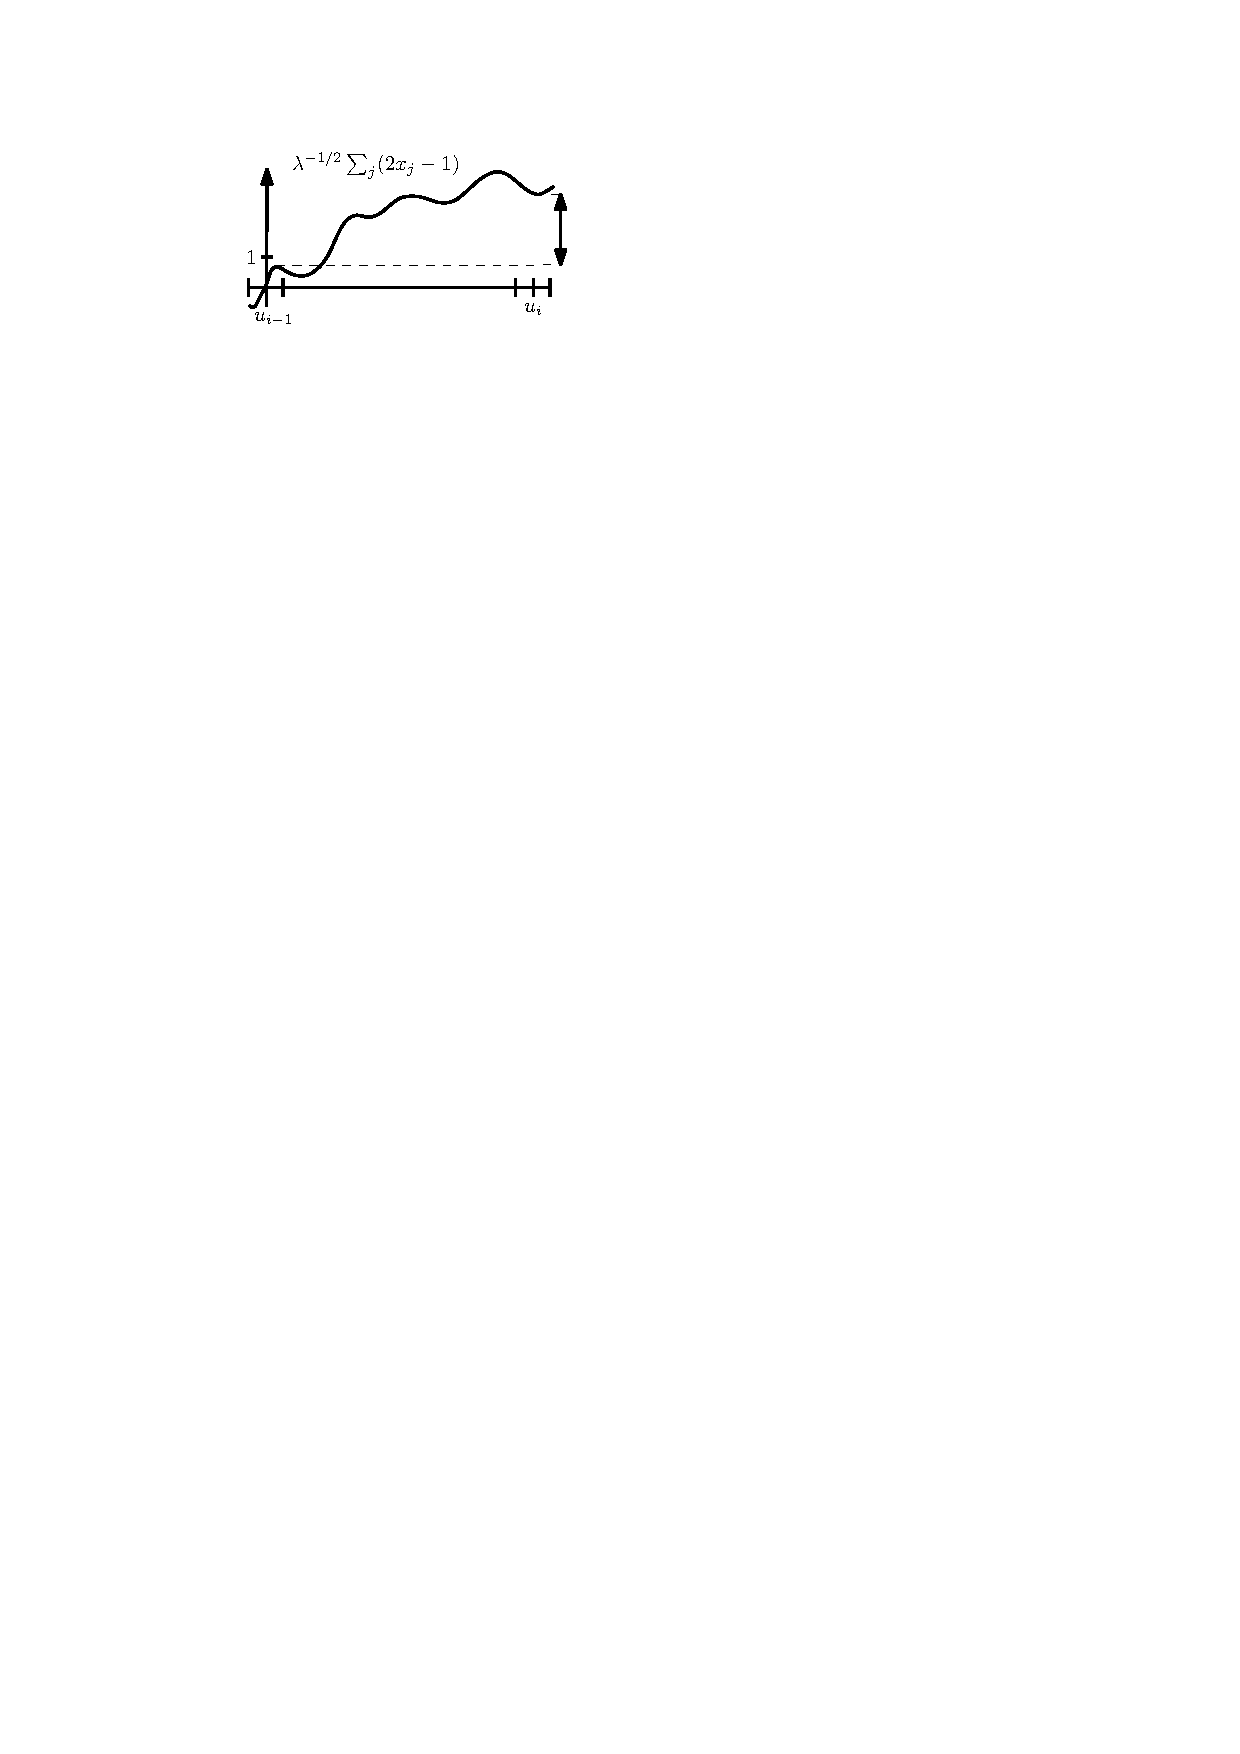
\includegraphics[scale=1]{robustbias}
	\caption{The length of the vertical arrow describes the robust bias
		associated with the block $\x(u_{i-1} + 1 : u_i)$.  The curve
		represents the partial sums $\lambda^{-1/2}\sum_j (2x_j-1)$,
		renormalized to equal 0 at $u_{i-1}$. We say that the robust bias
		is clear if it is at least 1, such as shown in the given example.}
	\label{fig:robust}
\end{figure}

Define $T_1=T_{1;\x,\xt}^{\lambda,\ell,c_1}:\Z^2\to\{0,1 \}$  by
\eqb \label{eq33}
T_1(k,k') =
\begin{cases}
	1 \qquad \disp \text{\,\,if\,\,} k' ,k \geq \ell - 1 \text{\,\,and\,\,}
	\sum_{i \in \mcl I_1} \op{sign}(s_i) \cdot \op{sign}(\wt s_i) >
	c_1 |\mcl I_1| \, , \\
	0 \qquad \text{otherwise}.
\end{cases}
\eqe

Define $d_2 := \lceil \ell / (\lambda C_1) \rceil$,
and let $\cI_2 \subset \{1 , \dots , d_1 \}$ be the set consisting
of the $\lceil \theta d_2 \rceil$ blocks which are contained in
$\x(k - \lceil \ell / C_1 \rceil + 1 : k)$ and which have the
largest robust bias.  Define
$T_2 = T^{\lambda , C_1 , \ell,c_1}_{2 ; \x , \xt} : \Z^2\to\{0,1 \}$ by
\eqbn
T_2(k,k') =
\begin{cases}
	1 \qquad \displaystyle\text{\,\,if\,\,} k' , k \geq \ell - 1
	\text{\,\,and\,\,} \sum_{i\in\mcl I_2}
	\op{sign}(s_i) \cdot \op{sign}(\wt s_i) > c_1 |\mcl I_2|,\\
	0 \qquad\text{otherwise}.
\end{cases}
\eqen
\begin{definition} \label{def10}
	Define $T = T^{\lambda , C_1 , \ell,c_1}_{\x , \xt} : \Z^2 \to \{0 , 1 \}$ by
	$$T(k,k'):=T_1(k,k')\wedge T_2(k,k').$$
	Note that the value of $T^{\lambda,C_1,\ell,c_1}_{\x,\xt}(k,k')$ depends
	on $\x$ and $\xt$ only on the windows $\x(k - \ell + 1 : k)$
	and $\xt(k' - \ell + 1 : k')$, respectively.
\end{definition}
The purpose of requiring both $T_1(k,k')=1$ and $T_2(k,k')=1$ is the following. We require $T_1(k,k')=1$ since this condition makes it very unlikely that the test gives false positives, due to the large number of blocks used in the test $T_1$. However, if we had only required $T_1(k,k')=1$ (not also $T_2(k,k')=1$) the long length $\ell$ of the string would have made it rather likely that $|f(k_*)-\tau_2|$ equals a large multiple of $\log^{1/3}(n)$ in the second alignment step, due to the effect described in Figure \ref{fig2}. We require $T_2(k,k')=1$ to make sure that $|f(k_*)-\tau_2|$ is typically not more than a \emph{small} constant multiple of $\log^{1/3}(n)$, on the event that we have a true positive test.
\begin{lemma} \label{lem:c}
	Let $K_1 \in \sigma (\omega)$ be the event that the trace is
	$\lambda$-aligned in $[k - \ell + 1 , k]$.
	There are $\delta , \lambda_0,c_1 > 0$ depending only on $q$ such that for all $C_1\geq 1$, we have
	$\P_\x \big[T^{\lambda,C_1,\ell,c_1}(k,f(k)) = 1 | K_1\big] \geq \delta$ when $\lambda > \lambda_0$
	and $\x$ is such that all the blocks in $\cI_1$ and $\cI_2$ have clear
	robust bias.
\end{lemma}

\begin{proof}
	Let $j_1 (i)$ (resp.\ $j_2 (i)$) denote the position of the
	first (resp.\ last) bit in $\x$ that was copied to a
	position in block $i$ of $\xt$.  Let $m_i$ denote the number of
	bits in block $i$ of $\xt$ that were copied from $\xt$.
	Let $\cH$ be the $\sigma$-field containing each $j_1 (i), j_2 (i)$
	and $m_i$ for all $i \leq d_1$. Observe that $K_1\in\cH$. Under $\P_\x$, conditional on $\cH$,
	the $\lambda + 1 - m_i$ or $\lambda - m_i$ non-copied bits in the $i$th block of $\xt$ are
	all inserted bits, therefore are i.i.d.\ mean zero Rademacher variables
	(and independent as $i$ varies as well).  Their sum is well approximated
	by a normal with mean zero and variance $\lambda - m_i$.
	
	Fix $i$ and without loss of generality assume $s_i > 0$, which if
	the $i$th block has clear robust bias implies $s_i > \lambda^{1/2}$.
	Conditioned on $\cH$,
	the copied bits in the $i$th block are $j_1 (i)$ and $j_2 (i)$ together
	with $m_i - 2$ locations uniformly chosen from among all size $(m_i - 2)$ subsets of $\Z\cap[j_1 (i) + 1 , j_2 (i) - 1]$.  On $K_1$, we know $j_1 (i)$ and $j_2 (i)$
	are within $\lambda / 100$ of $u_{i-1}$ and $u_i$ respectively,
	and when the $i$th block of $\x$ has clear robust bias, the number
	of positive bits of $\x$ in this range is at least $(j_2(i)-j_1(i) +1+\lambda^{1/2})/2$.  Therefore the sum of the copied values of
	$2x_j - 1$ is approximately normal with mean at least $m_i \lambda^{-1/2}$
	and variance $m_i$, independently of the sum of the non-copied bits.
	
	Adding the copied and non copied bits gives approximately a normal with
	mean at least $m_i \lambda^{-1/2}$ and variance $\lambda$.  We know that
	$m_i > \lambda p/2$ with probability tending to~1 as $\lambda \to \infty$.
	Therefore, when all the blocks in
	$\cI_1$ and $\cI_2$ have clear robust bias, there is a $\lambda_0$ and a $c_1 > 0$ such that for all
	$\lambda > \lambda_0$, $\P_\x [\sign (s_i) = \sign (\wt s_i) > 0]
	\geq 1/2 + c_1$.  Furthermore under $\P_\x$, this holds independently
	over all the blocks.  In this case the expected sum over $i \in \cI_1$ of
	$\sign (s_i) \cdot \sign (\wt s_i)$ is at least $2 c_1 |\cI_1|$,
	conditional on $\cH$, when $K_1$ holds.  By Markov's inequality, we obtain
	a positive lower bound $\delta_0$ on $\P_\x [T_1 (k , f(k)] = 1 | \cH)$ when
	$K_1$ holds.  The same holds for $T_2$, and furthermore, by the Harris inequality\footnote{Recall that the Harris inequality says the following: Let $d\in\N$, let $S=(S_1,\dots,S_d)$ be a collection of independent real-valued random variables, and let $f$ and $g$ be increasing functions of $S$, i.e., $f(s_1,\dots,s_k)\geq f(s'_1,\dots,s'_k)$ if $s_1\geq s'_1,\dots,s_k\geq s'_k$, and similarly for $g$. Then $\E[f(S)g(S)]\geq \E[f(S)]\E[g(S)]$.} \cite{harris60,gg99},
	\begin{eqnarray*}
		\P_\x \Big [ T_1(k,f(k)) = 1 \mbox{ and } T_2 (k,f(k)) = 1 | \cH \Big ]
		& \geq & \P_\x [T_1(k,f(k)) = 1 | \cH] \\
		&& \cdot \; \P_\x [T_2(k,f(k)) = 1 | \cH],
	\end{eqnarray*}
	because we consider increasing events in conditionally independent variables $\sign (s_i) \cdot \sign (\wt s_i)$.  Taking $\delta =
	\delta_0^2$ and removing the conditioning on $\cH$ finishes the proof.
\end{proof}

\subsection{Choice of constants} \label{ss:choice}

The test $T$ and a number of events used in its analysis depend on
the parameter $C_1$.  Throughout the remainder of Appendix~\ref{sec:test2},
the constant $C_1$ remains as a free parameter.  To make the arguments
in the rest of the paper more transparent, we discuss in advance what
relationship is needed between $C_1$ and the constants in
Theorem~\ref{th:align}, and what choices will be made to ensure the
necessary inequalities.
%
A constant $\ct \ll 1$ will be small enough to be a witness for $c$
in Lemmas~\ref{prop18} and~\ref{prop11} as well as ensuring some
properties of the the random walks $\{ g(j) \}$ and $\{ f(j) \}$.
The constant $C_1$ will be sufficiently large to ensure that a number
of other asymptotic behaviors have kicked in.  In particular, we will take
$C_1 = 64 \ct^{-12}$.  A constant $\chuge$ will then be chosen that is
large compared to $C_1$.  The constants in Theorem~\ref{th:align} will
be chosen as follows.
%
$$\begin{array}{lcr}
\cback & = & {\disp 5 \, \chuge} \\[1ex]
\calign & = & {\disp \frac{1}{10} \, \chuge } \\[2ex]
\ctrue & = & {\disp \frac{2 \ct^{-1}}{C_1^{10/3}} \, \chuge } \\[4ex]
\cfalse & = & {\disp \frac{\ct}{2 C_1^{5/3}} \, \chuge } \\[3ex]
\cavg & = & {\disp \frac{2}{C_1^2} \, \chuge }
\end{array}$$
With $\chuge \gg C_1 \gg \ct^{-1} \gg 1$, the necessary inequalities
will then result from the relation between the powers of $C_1$ in
$\ctrue, \cfalse$, and $\cavg$.
%
We conclude this subsection by specifying $C_1$ and $\ct (q)$.
%
\begin{definition} \label{def3}
	In the remainder of the paper let $\theta \in (0,1/10)$ be given by \eqref{eq18}, let $c_1\in(0,1/10)$ be as in Lemma \ref{lem:c}, let $C_1=64\wt c^{-12}$ with $\wt c$ as we define next, and let $\ct >0$ be a constant depending only on $q$ and which is sufficiently small such that following properties hold.
	\begin{enumerate}[$(i)$]
		\item $\ct$ is smaller than the values of $c$ in the conclusion of
		Lemmas~\ref{prop18} and~\ref{prop11},
		\label{rr:i}
		\item $\ct \leq c_1^2 \theta / 10$,
		\label{rr:ii}
		\item recalling~\eqref{eq25}, the probability that the robust bias
		of the block $\x (u_{i-1} + 1 : u_i)$ is clear is at least $4 \theta$
		when $\lambda \geq (10 \ct)^{-1}$, and the constant $\lambda_0$ from Lemma \ref{lem:c} satisfies $\lambda_0<(10\ct)^{-1}$,
		\label{rr:iii}
		\item $\Var(g(1) - g(0)) \leq (10 \ct)^{-1}$,
		\label{rr:iv}
		\item $\P_\omega [f(1)-f(0) > \ell] \leq \exp(-10 \ct \ell)$ and
		$\disp \P_\omega [|f(k + u) - f(k) - u| \geq a] \leq
		\exp \left (- \frac{10 \ct a^2}{u} \right )$ for any $u\in\{1,2\dots \}$, and
		\label{rr:v}
		\item $2 / \ct^3 - \ct^{15} / 8 > 7 \csep$.
		\label{rr:vi}
	\end{enumerate}
\end{definition}

\subsection{Estimates related to the test $T$} \label{ss:T}

In the remainder of the appendix we prove various estimates related to
the test $T$.  The following lemma will be used to lower bound the
probability that the test gives true positives, i.e., it will be used
to lower bound $\P_{\x}[ T(k,f(k)) = 1 ]$.

In Definitions \ref{def2} and \ref{def5} below we define two events
$\Rhat (k,\wh k)$ and $\Rc (k)$.  These are measurable with respect
to $\x$, that is, they depend only on the input; their definitions
contain probabilities with respect to the channel but do not depend
on the sample $\omega$.
They depend on the parameters $\lambda$ and $\ell$; additionally
$\Rc (k)$ depends on $C_1$.
%
When we choose an interval for alignment, we will require
that the right end-point $k_*$ satisfies $\Rc (k_*)$
and $\Rhat (k_*,\wh k)$ for all $\wh k$ in a given interval.
From this we will deduce an upper bound for the probability of
false positives and a lower bound for the probability of true positives.
Occurrence of the event $\Rhat (k,\wh k)$ ensures that the $\ell$-windows
in $\xt$ ending between $f(\wh k)$ and $f(\wh k+1)$ are sufficiently
different from $\x(k_* - \ell + 1 : k_*)$ that the test $T(k,i)$ is
unlikely to give a positive result when $i$ is close to $f(\wh k)$
instead being close to $f(k)$, as desired; see Figure~\ref{fig:k_*}.

\begin{figure}[b]
	\centering
	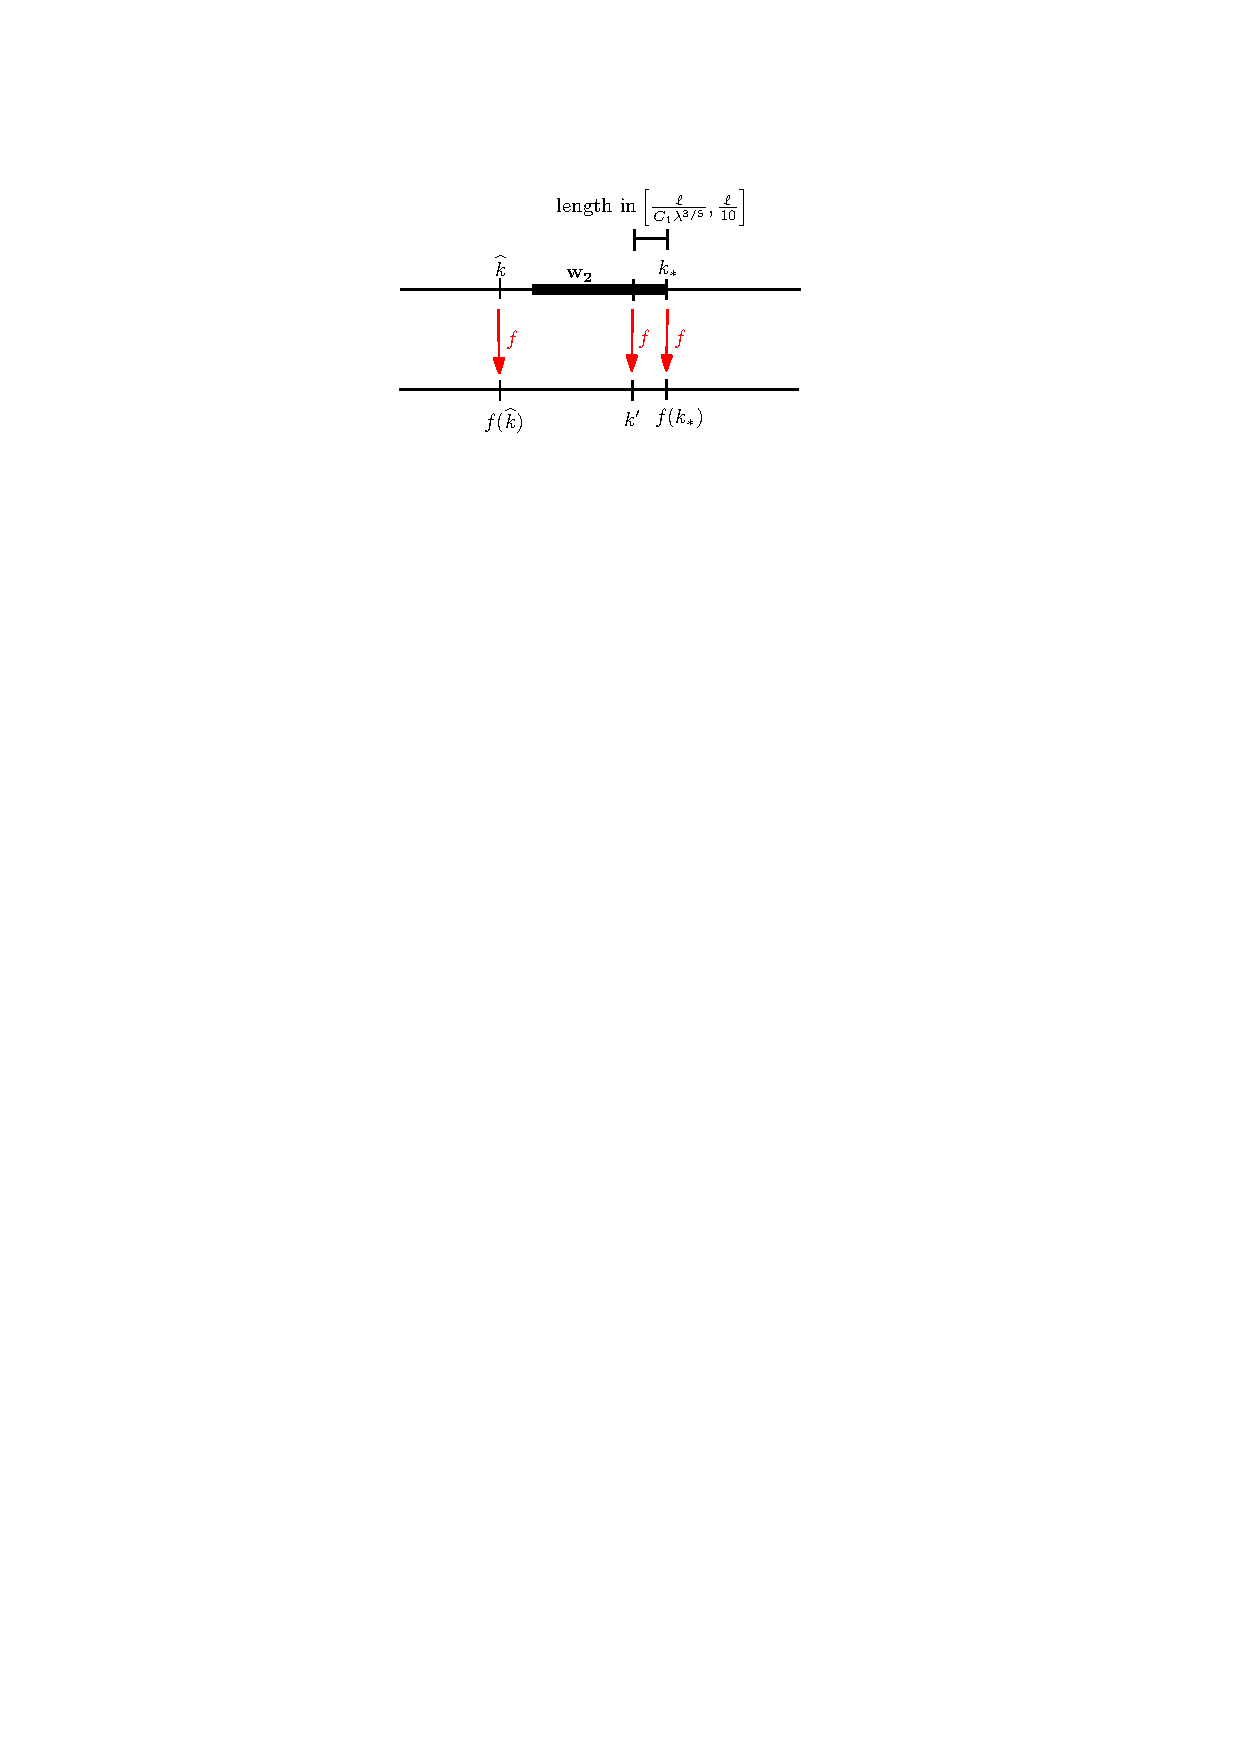
\includegraphics[scale=1]{findkstar}
	\caption{The right end-point $k_*$ of the interval used
		in the second alignment step is (roughly speaking) chosen such that
		$\P_{\bf x}[ T_1(k_*,f(\wh k))=1 ]\leq \exp(-\ct\ell/\lambda)$,
		$\P_{\bf x}[ T_2(k_*,k')=1 ]\leq \exp(-\ct\ell/(C_1 \lambda^{6/5}) )$,
		and $\P_{\bf x}[ T(k_*,f(k_*))=1 ]\geq \exp(-\ell/(\ct\lambda^2))$.
		See Definitions \ref{def2} and \ref{def5} for the precise requirements.}
	\label{fig:k_*}
\end{figure}

\begin{definition}
	For a fixed string $\x\in\mcl S$, $\ell\in\N$, $\lambda \in
	\{ 1,\dots,\lfloor \ell^{1/2}\rfloor \}$, and $k , \wh k \geq 2 \ell$,
	define the event $\Rhat (k,\wh k)=\Rhat_\x^{\lambda,\ell}(k,\wh k)$ to
	hold when
	$$\P_{\bf x} [E] < e^{- \ct \ell / \lambda},$$
	where
	$$E := \Bigg \{ \bigcup_{i=f(\wh k)}^{f(\wh k+1)}
	\{ T_1(k,i)=1 \} \cap E_{\ell; k, i} \, ;
	|g(i) - g(i - \ell)| < 11 \ell / 10  \Bigg \} \, . $$
	\label{def2}
\end{definition}

\begin{unremark}
	The event $\Rhat (k,\wh k)$ is measurable with respect to
	$\x (k - \ell + 1 : k)$ and $\x (\wh k - \lfloor 11 \ell / 10
	\rfloor : \wh k+2)$.  This ensures independence of the events
	$\Rhat (k_1 , \wh k_1)$ and $\Rhat (k_2 , \wh k_2)$ when $k_1$
	and $\wh k_1$ are sufficiently far from $k_2$ and $\wh k_2$.
	We will use this independence property and the following lemma
	to argue that with high probability we can find a $k_*$ in a
	given interval such that $\Rhat (k_*,\wh k)$ occurs for all
	$\wh k$ in a given larger interval.
\end{unremark}

\begin{lemma} \label{prop9}
	Define the $\sigma$-field $\cG_{k,\ell}$ by
	$$\cG_{k , \ell} = \sigma( x_i \, : \, i \not\in \{ k-\ell + 1 , \dots,
	k \}) \, .$$
	Then for all $\lambda>3$ and $\ell$ sufficiently large,
	\eqb \label{eq1}
	\mu \left [ \Rhat_\x^{\lambda,\ell} (k , \wh k)^c \, | \, \mcl G_{k,\ell}
	\right ] \leq \exp(- \ct \ell / \lambda).
	\eqe
\end{lemma}

\begin{proof}
	Observe that $\Rhat (k , \wh k)^c = \{ \P_{\bf x}[E] \geq
	\exp (- \ct \ell / \lambda) \}$.  We will show that for $\ell$ sufficiently large,
	\eqb \label{eq4}
	\P[ E \,|\,\cG_{k , \ell} ] \leq \exp(- 2\ct \ell/\lambda) \, .
	\eqe
	This is sufficient to complete the proof, because Markov's inequality and
	the identity $\E[ \P_{\bf x} [E] \, | \, \cG_{k , \ell} ] = \P [E \, | \, \cG_{k , \ell}]$ give
	$$ \mu \left [ \Rhat (k , \wh k)^c \, | \, \cG_{k , \ell} \right ]
	\leq \frac{\P [ E \, | \, \cG_{k , \ell} ]}{\exp(- \ct \ell/\lambda)}
	\leq \exp(- \ct \ell/\lambda) \, .$$
	
	Assume $\wh k < k$; the case $\wh k\geq k$ can be treated similarly.
	Let $i_1 , \dots , i_{|\cI_1|}$ be an enumeration of the elements
	of $\cI_1$ in increasing order.  Let $i_0 = k - \ell$.
	Define the filtration $\cF_j$, $j=0,\dots,|\cI_1|$, by
	$$\cF_j = \sigma( \omega,\x(0:i_j), \x(k+1:\infty), \cI_1) \, .$$
	Observe that $\cF_0=\sigma(\omega,\cG_{k , \ell})$.
	For fixed $i\in\N$ let $M=(M_j)_{j\in\{0,\dots,|\cI_1| \}}$ be the
	stochastic process defined by the partial sums in~\eqref{eq33},
	with $f(\wh k) + i$ being the right end-point of the considered
	interval of the trace, i.e., $M_0=0$, and for $j=1,\dots,|\cI_1|$,
	$$M_j = \sum_{j'=1}^j \op{sign}\big(s_{i_{j'}} ( k,\ell,\lambda ) \big)
	\cdot \op{sign}\big(\wt s_{i_{j'}}( f(\wh k)+i,\ell,\lambda )\big)
	\,, $$
	where $s_{i_{j'}} ( k,\ell,\lambda )$ and $\wt s_{i_{j'}}( f(\wh k)+i,\ell,\lambda )$ are defined as in \eqref{eq37}.
	Observe that for each fixed $i$, the sequence $\{ M_j
	\one_{E_{\ell; k, f(\wh k) + i}} : 0 \leq j \leq | \cI_1 | \}$
	is a martingale on the filtration $\cF_j$ with increments bounded
	in magnitude by~1. The martingale property follows from the fact that
	$E_{\ell; k, f(\wh k) + i}\in\sigma(\omega)$, that
	$\wt s_{i_{j}} \in \cF_{j-1}$ on the non-overlapping event $E_{\ell; k, f(\wh k) + i}$, and that $\op{sign}(s_{i_{j}})$
	has expectation zero given $\cF_{j-1}$. The Azuma-Hoeffding inequality (\cite{hoeffding63,azuma67}) therefore gives $\P [M_j\one_{E_{\ell; k, f(\wh k) + i}} \geq t] \leq \exp ( - t^2 / (2j))$.  With
	$t = c_1 | \cI_1 |$ and $j = |\cI_1| $
	we may compute $t^2/(2j) = c_1^2 |\cI_1| / 2 = c_1^2 \theta \ell /
	(2 \lambda)$, whence
	\begin{eqnarray} \label{eq17}
	\P\left[ T_1(k , f(\wh k) + i) = 1 ; \, E_{\ell; k,  f(\wh k) + i} \, | \,
	\mcl G_{k , \ell} , \omega \right ]
	& = & \P \left [ M_{|\cI_1|} > c_1 | \cI_1 | ; \, E_{\ell; k, f(\wh k) + i}
	\, | \, \mcl G_{k , \ell} , \omega \right ] \\
	& \leq & \exp(- c_1^2 \theta \ell / (2 \lambda)) <
	\exp(- 3 \ct \ell / \lambda), \nonumber
	\end{eqnarray}
	where the last inequality follows from part~$(\ref{rr:ii})$ of Definition~\ref{def3}.
	Define $\cI' = | \{ f(\wh k) , \dots , f(\wh k+1) \} |$.  The
	inequality~\eqref{eq4} now follows from a union bound, using
	part~$(\ref{rr:v})$ of Definition~\ref{def3} and~\eqref{eq17}
	in the third inequality, with the last inequality following when
	$\ell$ is sufficiently large from $\lambda \leq \ell^{1/2}$.
	\begin{eqnarray*}
		\P[ E \,|\,\mcl G_{k , \ell} ]
		& \leq & \P \left [ \bigcup_{i = f(\wh k)}^{f(\wh k+1)}
		\{ T_1(k , i) = 1 \} \cap E_{\ell; k , i}\,\Big|\,\cG_{k , \ell} \right] \\
		& \leq & \P[ |\cI'| > \ell \, | \, \cG_{k , \ell} ] + \sum_{i=0}^{\ell - 1}
		\P\left[ T_1(k , f(k) + i) = 1 \, ; E_{\ell; k, f(\wh k)+ i} \, | \,
		\cG_{k , \ell} \right] \\
		& \leq & \exp(-\ct\ell) + \ell \exp(-  3 \ct \ell/\lambda) <
		\exp(-  2 \ct \ell / \lambda) \, .
	\end{eqnarray*}
\end{proof}

Part $(i)$ of the event $\Rc (k)$ defined just below will
ensure that the probability of true positives is sufficiently large.
Part $(ii)$ of the event will be used to bound from above the
probability that $|\tau_2-f(k_*)|>c\log^{1/3}n$ for some small constant $c$.
\begin{definition}
	Let $\x \in \mcl S$, $\ell \in \N$, $\lambda \in \{ 1, \dots , \lfloor
	\ell^{1/2}\rfloor \}$, $C_1\geq 1$, and $k\geq 2\ell$.  Define the event
	$\Rc (k) = \Rc_\x^{\lambda,C_1,\ell}(k) \in \sigma (\x)$ to occur if
	\begin{enumerate}[$(i)$]
		\item $\P_{\x}[ T(k,f(k))=1;\,
		|f(k) - f(k - \lfloor 11 \ell / 10 \rfloor)| > \ell ]
		> \exp(-\ell/(2\ct\lambda^2))$, and
		\item for $\cI'=\cI'_1\cup\cI'_2$ with
		\eqbn
		\begin{split}
			\cI'_1&:=\left\{
			k'\in\N\,:\,g(k')\in
			\{
			k-\lfloor \ell/10\rfloor,
			\dots,
			k- \lfloor \ell/(C_1\lambda^{3/5})\rfloor
			\}
			\right\},\\
			\cI'_2&:=\left\{k'\in\N\,:\,
			g(k')\in\left\{
			k+ \lfloor\ell/(C_1\lambda^{3/5})\rfloor,\dots,
			k+\lfloor\ell/10\rfloor
			\right\}\right\},
		\end{split}
		\eqen
		we have
		\eqbn
		\begin{split}
			\P_{\x}&\left[ \bigcup_{k' \in \cI'} \{T_2(k,k')=1\}\cap
			\{
			|f(k-\lfloor \ell/10 \rfloor-1)-f(k-\ell-2\lfloor \ell/10 \rfloor)|>\ell
			\} \right]\\
			&\qquad\qquad\qquad\qquad\qquad\qquad\qquad\qquad\qquad\qquad\qquad<\exp(-\ct\ell/(C_1\lambda^{6/5}) ).
		\end{split}
		\eqen
	\end{enumerate}
	\label{def5}
\end{definition}

\begin{unremark}
	In fact $\Rc (k)$ is measurable with respect to  $\x( k-\ell-2\lfloor
	\ell/10 \rfloor : k + \lfloor \ell / 10 \rfloor )$.
\end{unremark}

\begin{lemma}
	For  $\ell\in\N$ sufficiently large, $\lambda \in \{ 10 \lceil
	\ct^{-1} \rceil,\dots,\lfloor \ell^{1/2}\rfloor \}$,
	and $C_1\geq 1$,
	\eqb \label{eq:mu}
	\mu\left[\Rc_\x^{\lambda,C_1,\ell}(k)^c\right]
	<\exp(-\ct \ell/(C_1\lambda)).
	\eqe
	\label{prop19}
\end{lemma}

\begin{proof}
	We verify separately that each property $(i)$ and $(ii)$ of
	Definition \ref{def5} fail on a set of $\mu$-measure at most
	half the quantity on the right-hand side of~\eqref{eq:mu}.
	We claim that $(i)$ holds whenever all blocks in
	$\cI_1$ and $\cI_2$ have clear robust bias.  To see this
	let $K_1$ be the event that the trace is $\lambda$-aligned in
	$[k - \ell + 1 , k]$, and let $K_2$ be the event that
	$|f(k) - f(k - \lfloor 11 \ell / 10 \rfloor)| > \ell$.
	Then
	$$\P_\x [T(k,f(k)) = 1] \geq P_\x (K_1) \P_\x [T(k,f(k)) = 1 | K_1].$$
	Lemma~\ref{prop18} gives us $\P_\x [K_1] \geq \exp ( - \ell /
	(10 \ct \lambda^2))$ and Lemma~\ref{lem:c} gives us
	$\P_\x [T(k,f(k)) = 1 | K_1] \geq \delta$ when all the blocks in $\cI_1$
	and $\cI_2$ have clear robust bias.  Thus, when all the blocks have
	clear robust bias,
	$$\P_\x [T(k , f(k)) = 1 ; K_2] \geq \delta \exp \left (
	-\frac{\ell}{10 \ct \lambda^2} \right ) - \P_\x [K_2^c] \, .$$
	By part~$(\ref{rr:v})$ of
	Definition~\ref{def3} and the hypothesis $\lambda \geq 10 \ct^{-1}$
	gives
	\begin{eqnarray*}
		\P \left[|f(k) - f(k-\lfloor 11\ell/10\rfloor)| \leq \ell \right]
		& \leq & \P \left[|f(k) - f(k-\lfloor 11\ell/10\rfloor) - (11 \ell / 10) |
		\geq \ell / 10 \right] \\
		& \leq & \exp \left ( -\frac{10 \ct (\ell / 10)^2}{12 \ell / 10} \right ) \\
		& = & \exp \left ( - \frac{\ct \ell}{12} \right ) \\
		& \leq & \frac{1}{2} \exp \left ( - \frac{\ell}{\ct \lambda^2} \right ) \, ,
	\end{eqnarray*}
	proving the claim.
	
	To see that all blocks in $\cI_1$ and $\cI_2$ have clear robust bias
	except on a set of $\mu$-measure at most half the right side of~\eqref{eq:mu},
	we require the following large deviation bound for binomial variables:
	\eqb \label{eq:KL}
	\P [\Bin (n , 4 \theta) \leq 2 \theta n]
	\leq \exp (- 2 (1 - \ln 2) n \theta) < \exp (- n \theta / 2) \, .
	\eqe
	To derive this, begin with the well-known Kullback–-Leibler bound for
	$Z \sim \Bin (n,p)$ and $r \leq p$,
	$$\frac{1}{n} \log \P [Z \leq rn] \leq r \log \frac{p}{r} + (1-r)
	\log \frac{1-p}{1-r} \, ,$$
	which may be obtained, for instance, by applying Markov's inequality
	with $\E e^{\lambda Z} = (1-p+pe^\lambda)^n$ and $\lambda = \log(r/p)
	- \log((1-r)/(1-p))$.  Plugging in $p = 4 \theta$ and $r = 2 \theta$
	yields, for $\theta < 1/4$,
	$$\frac{1}{n} \log \P [\Bin (n , 4 \theta) \leq 2 \theta n]
	\leq h(\theta) := \log \frac{1-4\theta}{1 - 2\theta}
	+ 2 \theta \log \frac{2 - 4\theta}{1 - 4\theta} \, .$$
	Observing that $h'(0) = - 2 (1 - \ln 2) < -1/2$ and $h'' < 0$ on $(0,1/4)$
	then establishes~\eqref{eq:KL}.
	
	Each block has a clear robust bias with probability at least
	$4 \theta$ by part~$(\ref{rr:iii})$ of Definition~\ref{def3}
	and the requirement $\lambda > 10\ct^{-1}$.
	Furthermore, the event that this holds
	is independent for any pair of blocks which are not adjacent.
	Applying~\eqref{eq:KL} to the $\ell / (2 \lambda C_1)$ even numbered
	blocks from among which $\cI_2$ was chosen shows that at least
	$\theta \ell / (\lambda C_1)$ of these, hence all blocks in $\cI_2$,
	have clear robust bias except on an event of probability at most
	$\exp(- \theta \ell / (4\lambda C_1)) < \exp(-2 \ct \ell / (C_1 \lambda))$.
	For $\cI_1$ the same bound holds without the factor of $C_1$ in the
	denominator.  These negative exponents are both at least twice the
	negative exponent on the right side of~\eqref{eq:mu}, therefore sum to
	at most half the right side of~\eqref{eq:mu} once $\ell$ is sufficiently large.
	
	Now we consider $(ii)$ of Definition \ref{def5}. Let $k'_1$ (resp.\ $k'_2$) be the largest (resp.\ smallest)
	element of $\cI'_1$ (resp.\ $\cI'_2$), and define $d = \lfloor \ell /
	(2C_1 \lambda^{3/5}) \rfloor$. Recalling Definition~\ref{def4} and
	Lemma~\ref{prop11}, we have for $\ell$ sufficiently large,
	\eqbn
	\begin{split}
		\P[ E_{\lfloor\ell/C_1\rfloor,k,k'_1}^c ]
		&\leq \P\left[ E_{\lfloor\ell/C_1\rfloor,k,f(k)-d }^c \right]
		+ \P[ |f(k)-k'_1|<d ]\\
		&\leq \ct^{-1}\exp(-10\ct d^2C_1/\ell) + \exp(- \ct d )\\
		&< \ct^{-1}\exp(-2\ct\ell/(C_1\lambda^{6/5})) \,.
	\end{split}
	\eqen
	Similarly, $\P [ E_{\lfloor \ell / C_1 \rfloor , k , k'_2}^c ]
	\leq \ct^{-1} \exp(-2 \ct \ell / (C_1\lambda^{6/5}))$.
	We also have $\P[ \left | \cI' \right| \geq \ell ] < \exp(-\ct \ell)$ and $\P[ f(k)\geq k'_2 ]=\P[ f(k)=f(k+d ) ] \leq \exp(-10\wt c d)$, where the last inequality follows from part $(\ref{rr:v})$ of Definition \ref{def3}. Define the event $E\in\sigma(\omega)$ by
	$$ E = E_{\lfloor \ell / C_1 \rfloor , k , k'_1} \cap
	E_{\lfloor\ell/C_1\rfloor,k,k'_2}\cap \left\{ \left| \cI'\right|
	< \ell \right\}
	\cap \{f(k)<k'_2 \}, $$
	and observe that
	\eqb
	\begin{split}
		\P[E^c]=\P_{\bf x}[E^c] < 3\ct^{-1}\exp(-2\ct\ell/(C_1\lambda^{6/5})).
	\end{split}
	\label{eq34}
	\eqe
	By a union bound,
	\eqb
	\begin{split}
		\P_{\x}&\left[ \bigcup_{k' \in \cI'} \{T_2(k,k')=1\}\cap \{|f(k-\lfloor \ell/10 \rfloor)-f(k-\ell-2\lfloor \ell/10 \rfloor)|>\ell\} \right]\\
		&\qquad\qquad \leq \P_{\x}\left[ \bigcup_{k' \in \cI'}
		\{T_2(k,k')=1\}\right]\\
		&\qquad\qquad \leq \P_\x[E^c]
		+ \sum_{j=0}^{\ell-1} \P_{\x}\left[T_2(k,k_2'+j)=1;\,E\right]
		+\P_{\x}\left[T_2(k,k_1'-j)=1;\,E\right].
	\end{split}
	\label{eq29}
	\eqe
	We bound the first term on the right side of \eqref{eq29}
	by~\eqref{eq34}.  To bound the other terms on the right side
	of~\eqref{eq29}, observe that the event $E_{\lfloor \ell / C_1 \rfloor , k , k'_2}\cap\{ f(k)<k'_2 \}$
	can occur only via~$(i)$, not~$(ii)$, in Definition~\ref{def4}.
	Thus $E_{\lfloor \ell / C_1 \rfloor , k , k'_2}$ implies
	$E_{\lfloor \ell / C_1 \rfloor , k , k'_2+j}$ for
	$j \in \{0 , \dots , \ell - 1 \}$.  This implies that no
	bit of the original string was copied to the respective
	block of the trace.  Repeating the martingale argument in the
	proof of Lemma~\ref{prop9}, Azuma's inequality gives
	\eqb
	\begin{split}
		\P\left[ T_2(k,k_2'+j)=1;\,E\right]
		&\leq \exp\big( - (c_1|\cI_2|)^2/(2|\cI_2|)\big)\\
		&\leq \exp\big( -c^2_1 \ell\theta /(2.1\lambda C_1)\big)
		\leq \exp( -4\ct\ell/(C_1\lambda) ).
	\end{split}
	\label{eq32}
	\eqe
	Markov's inequality gives further that except on a set of
	$\mu$-measure $\exp( -2\ct\ell/(C_1\lambda) )$ we have
	$$ \P_\x\left[ T_2(k,k_2'+j)=1;\,E\right]
	\leq \exp( -2\ct\ell/(C_1\lambda) ).  $$
	A similar result holds for the terms on the form $\P_{\x} \left [
	T_2(k , k_1'-j) = 1; \, E \right ]$ on the right side of~\eqref{eq29}. Therefore, except on an event of $\mu$-measure $2 \ell \exp(
	-2 \ct \ell / (C_1\lambda) ) < \exp(-\ct \ell / (C_1\lambda))$ for $\ell$ sufficiently large, we have
	\eqbn
	\begin{split}
		\P_{\x}&\left[ \bigcup_{k' \in \cI'} \{T_2(k,k')=1\}
		\cap \{|f(k-\lfloor \ell/10 \rfloor) -
		f(k-\ell-2\lfloor \ell/10 \rfloor)| > \ell\} \right]\\
		&\qquad\leq 3\ct^{-1}\exp(-2\ct\ell/(C_1\lambda^{6/5}))
		+ 2\ell \exp( -2\ct\ell/(C_1\lambda) )
		\leq \exp(-\ct\ell/(C_1\lambda^{6/5}) ).
	\end{split}
	\eqen
\end{proof}


\section{Existence of good positions} \label{sec:find}

Several more technical lemmas and a somewhat intricate definition
are needed to finish proving Theorem~\ref{th:align}.  To motivate
these, we first describe the rest of the proof.  The determination
of $(k_* , \tau_2)$ begins with construction of the rough approximation,
$\tau_1$.

Set $\ell = \Theta (\log^{5/3} n)$, $\lambda = \lfloor\ell^{2/5}\rfloor =
\Theta (\log^{2/3} n)$, and the constant $C_1$ to the value
chosen in Appendix~\ref{ss:choice}.  Slide an $\ell$-window
from left to right in the trace until the test
$T(k - 9 \chuge \log n , k')$ produces a value of~1, and let $\tau_1$
be the value of $k'$ at which this first occurs.  Define $\tau_1$
to be $\infty$ if this fails to occur for all $k' \leq 2 n$.

What we need from $\tau_1$ is that the true positive rate for aligning
within $9 \chuge \log n$ is at least $\exp (-c \log^{1/3} n)$ and that
the false positive rate is at most a similar but smaller function of
the same form, $\exp (-C \log^{1/3} n)$ for $C \gg c$.  However, and
this is crucial, we need this to hold not only in the space $\P_\mu$
but in the space $\P_\x$ for all strings $\x$ other than those in a
``bad'' set which must have measure $o(1/n)$ and therefore be much
smaller than $\exp (- \Theta (\log^{1/3} n))$.

Conditioning on a positive alignment $\tau_1 \approx f(k - 9 \chuge \log n)$,
we now retest to find an alignment of a carefully chosen position $k_*$,
accurate to within $\Theta (\log^{1/3} n)$.  Set $\ell  = \Theta (\log^{1/3} n)$ and $\lambda = \Theta (1)$, with
the same value of $C_1$ as before.  With $\ell$ this small, we can no
longer expect most strings $\x$ to be free of bad spots where the
proportion of traces producing false positive alignments is intolerably
high.  For this reason, we will find a $k_* \in [k - 5 \chuge \log n ,
k - 4 \chuge \log n]$ such that we can run the test $T(k_* , k')$ over
a window of length $\Theta (\log n)$ sitting between $\tau_1$ and
$\tau_1 + 9 \chuge \log n$.

The argument used to construct $(k_* , \tau_2)$ is more elaborate but
similar to the argument used to construct $\tau_1$.  For this reason,
we use the same lemmas in both constructions.  Some elements of the
argument appear unnecessarily complicated in the case of $\tau_1$, but
it still saves on space and ideas not to duplicate the sequence of
lemmas.  With this in mind, we outline the sequence of lemmas.

The key definition is that of the ``good'' position, $k_3=k_*$.  This
definition takes as input the test parameter $\ell, \lambda$ and
$C_1$, as well as an interval $\cI$ of values of $k'$ over which the
test $T(k_3 , k')$ is performed.  The position $k_3$ is deemed good if
the quenched probabilities $\P_\x$ for true and false positives and the
quenched expectation $\E_\x$ of the truncated discrepancy
satisfy inequalities that will be used to prove~$(\ref{r:iii})-(\ref{r:v})$
of Theorem~\ref{th:align}.  The corresponding key lemma,
Lemma~\ref{prop2} below, gives a lower bound on the probability
of finding a good $k_3$ such that the $\ell$-window $[k_2 , k_3]$
lies within a specified interval $[k_1,k_4]$.  The bound will improve
as the ratio $b$ of the length of $[k_1,k_4]$ to the length of $[k_2,k_3]$
grows.  In the case of $\tau_1$ it is applied in the somewhat degenerate
situation that $b=1$ to prove that with high probability
we may take $k_3 = k_4$.

One further complication is that the restrictions on where to search
take place in the trace, not the message.  We would like to restrict
the search to positions $f(j)$ corresponding to $j$ in some interval
$[k_0 , k_5]$.  Values of $f$ are not known to the algorithm,
therefore $\cI$ is never guaranteed to be a subset of
$[f(k_0) , f(k_5)]$ and the probability estimates must include
a fudge term accounting for failure of this inclusion.  The lemma
is proved for all choices of $\cI$ satisfying some desired inclusion property with sufficiently high probability but in fact only two choices are
required, one when constructing $\tau_1$ and one when constructing
$\tau_2$.

\begin{definition}[good alignment position] \label{def1}
	Fix a string $\x$ and positive integers $k_0 \leq k_2 < k_3 \leq k_5$.
	Let $\ell := k_3 - k_2 + 1$ and $L := k_5 - k_0 + 1$, and assume $k_2-k_0>\ell$. Fix a constant
	$C \geq 1$ and a positive integer $\lambda \leq \ell^{1/2}$.  For every (possibly random) set $\cI \subseteq \N$ we define an event $A_{\cI}$ by
	%
	\eqb \label{eq35}
	A_{\cI} := \Big \{ f(k_3) \in \cI \subset \{f(k_0)
	,f(k_0)+1,\dots,f(k_5)
	\} \Big \} \cap \{ f(k_3)-\ell> f(k_0)+\lceil L/9 \rceil \},
	\eqe
	%
	and a random variable $\tau_{\cI}$ by
	%
	\eqb \label{eq:def tau}
	\tau_{\cI} = \inf\{ k' \in \cI \, : \, T(k_3 , k') = 1 \} \, ,
	\eqe
	where $T = T_{\x , \xt}^{\lambda , C , \ell,c_1}$.  The infimum of
	the empty set is considered to be $+\infty$.
	Define the event $\good(k_3) = \good (k_0, k_2, k_3, k_5, \lambda, C, \x)$
	to hold if the following three properties $(i)-(iii)$ are satisfied for all (possibly random) $\cI$, for all positive integers $a \leq \ell$, and for all events $A_\cI^{(1)}$ and $A_\cI^{(2)}$ which satisfy
	\eqbn
	\begin{split}
		&A_\cI^{(1)}\cap A_\cI^{(2)}\subset A_\cI,\qquad
		\P_\x\big[\big(A_\cI^{(2)}\big)^c\big]\leq\exp(-\ell^2),\\
		&A_\cI^{(1)}\in \cG_{ f(k_0)+\lceil L/9 \rceil }^{k_5},\qquad
		\P_\x\big[A_\cI^{(1)}\big]>\exp\big(-\ell/(2\wt c\lambda^2)\big).
	\end{split}
	\eqen
	\begin{enumerate}[$(i)$]
		\item $\disp \P_{\bf x}[|k_3 - g(\tau_{\cI})| > a;
		\tau_{\cI} < \infty ; A_{\cI}]
		< 2L \exp(-\ct \ell / \lambda) + 3 \ct^{-1} \exp(- \ct a^2 / \ell)$,
		\item $\P_{\x} [\tau_{\cI} < \infty ; A_{\cI}] > \frac{1}{2} \exp(-\ell / (\ct \lambda^2))$, and
		\item $\displaystyle \E_{\x} [|k_3 - g(\tau_{\cI}) | \1_{A_{\mathcal I}} \1_{|k_3 - g(\tau_{\cI})|
			\leq \ell / 10 } \, | \, \tau_{\cI} < \infty ] \leq
		\frac{3 \ell}{2C \lambda^{3/5}}$\,.
	\end{enumerate}
\end{definition}

\begin{unremarks}
	%~~\\[-6ex]
	\begin{enumerate}[1.]
		\item The random variable $\tau_{\cI}$ is a stopping time with respect
		to the filtration $\{ \cG_j^{k_5} \}$.
		\item  The event $\good (k_3)$ is measurable with respect
		to $\x(0:k_5)$, since $\tau_{\cI}$ is bounded above by the greatest element of $\cI$ on the event that $\tau_{\cI}<\infty$, which implies that on the event $A_{\cI}$, the probabilities $\P_\x$ and expectation $\E_{\x}$
		in~$(i)-(iii)$ depend on $\x$ only via $\x(0:k_5)$.
		\item The events $A_\cI^{(1)}$ and $A_\cI^{(2)}$ will be used in the second alignment step. If the event $A_\cI^{(1)}$ occurs then the first alignment was successful. We will need to bound from below the probability of a successful second alignment, given that the first alignment step was successful. When we do this it will be useful to know that $A_\cI^{(1)}$ depends mainly on the deletions and insertions far away from the alignment position $k_3$ in the second alignment step. The event $A_\cI^{(2)}$ has very high probability, so $\P_{\bf x}\big[\big(A_\cI^{(2)}\big)^c\big]$ is negligible, and we therefore allow this event to depend on the deletions and insertions close to $k_3$.
	\end{enumerate}
\end{unremarks}

\begin{lemma} \label{prop2}
	Let
	\eqbn
	\begin{split}
		&1\leq \ell \leq L,
		\qquad
		1 \leq b \leq L / \ell ,
		\qquad
		2 \ell \leq k_0 \leq k_1 < k_4 \leq k_5,\\
		\qquad
		&|k_4 - k_1| \geq b \ell-1,\qquad |k_5 - k_0| = L-1
	\end{split}
	\eqen
	be constants with values in $\N$. Assume $\ell$ is sufficiently large, and that $C \geq 1$ and
	$\lambda \in \{ 1, \dots , \lfloor \ell^{1/2} \rfloor \}$ satisfy
	\eqb \label{eq42}
	2\frac{1}{\wt c\lambda^2} < \frac{\wt c}{C \lambda^{6/5} } \, .
	\eqe
	Then the $\mu$-measure of $\x$ such that
	$\good (k_0, k_2, k_3, k_5, \lambda, C, \x)$ holds for some
	$k_1 \leq k_2 < k_2 + \ell - 1 = k_3 \leq k_4$ is at least
	least $1 - L^b \exp(-\ct b \ell / (10 C \lambda))$.
\end{lemma}

\begin{figure}[!h]
	\centering
	\framebox{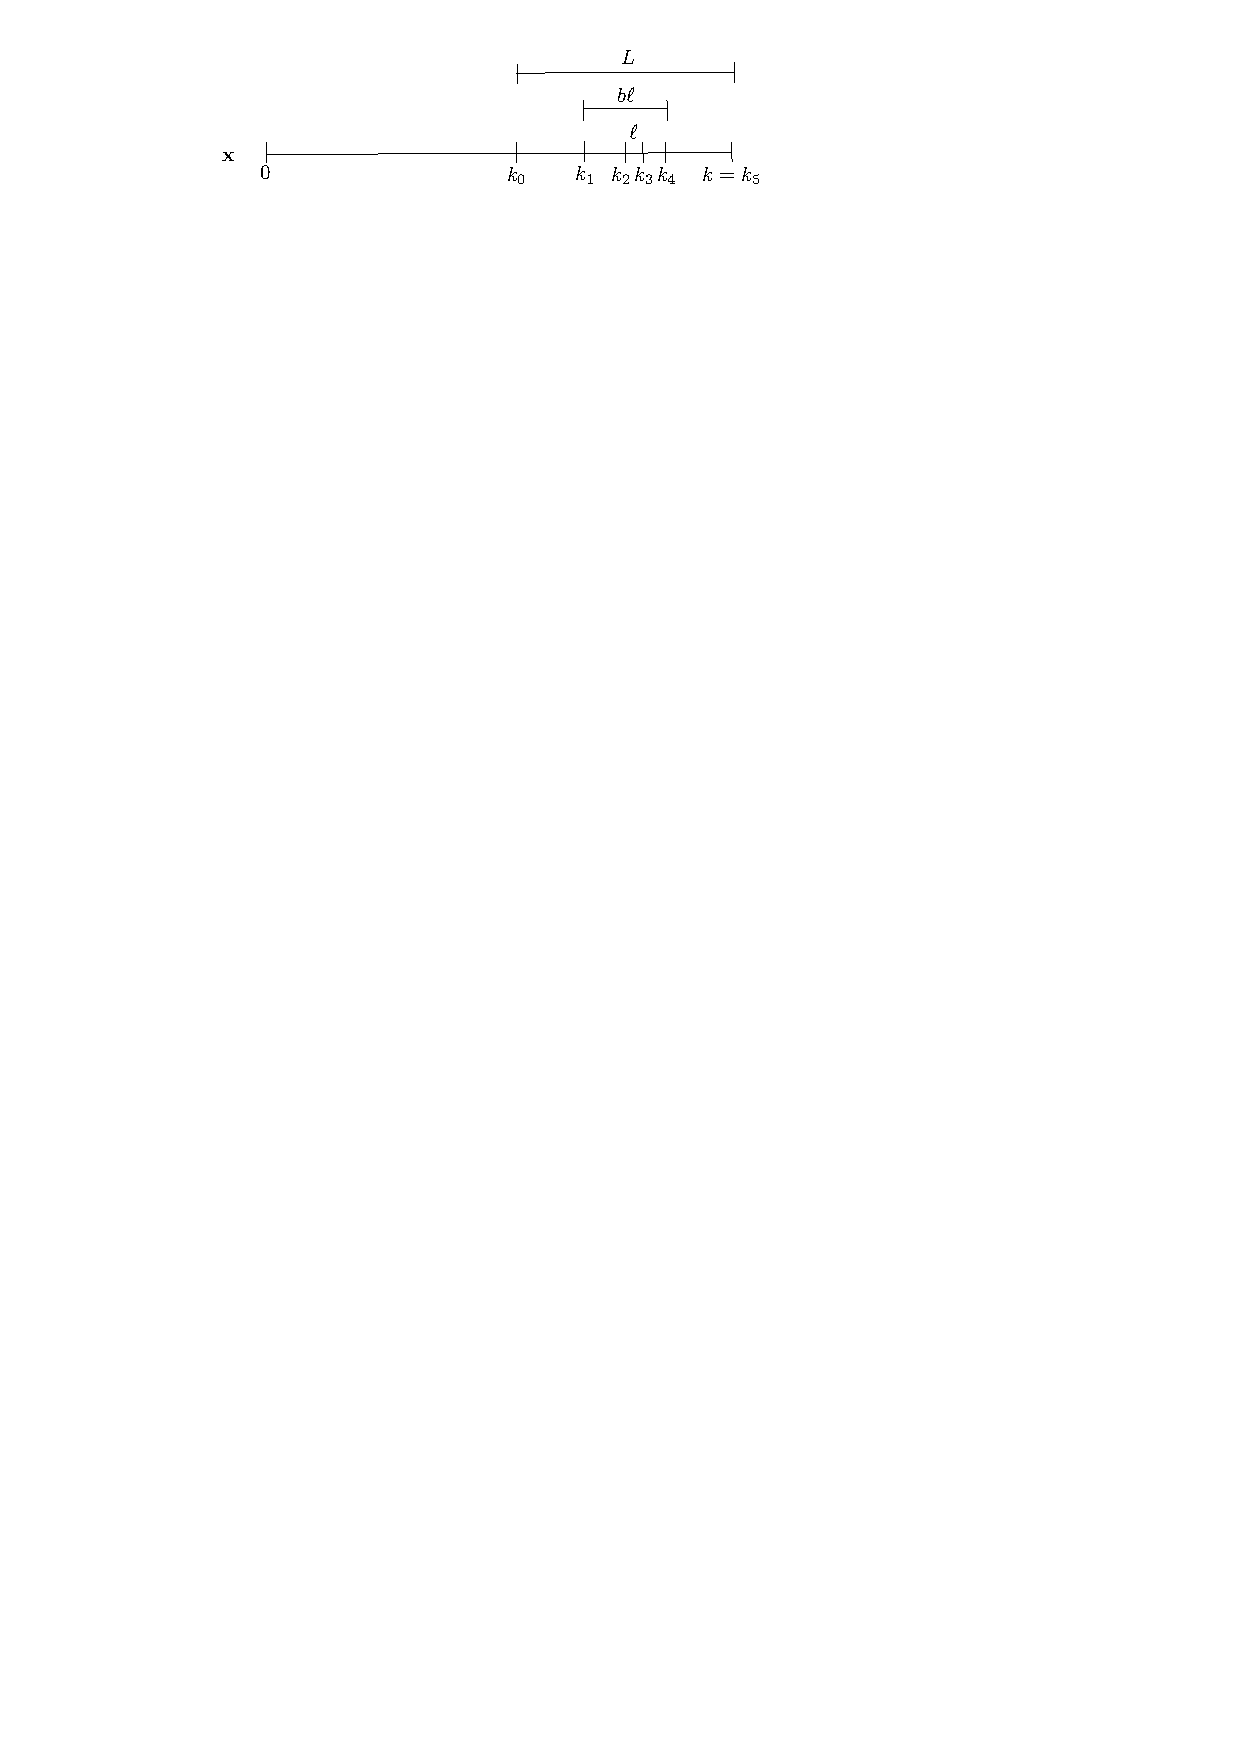
\includegraphics[scale=1]{intervals0}}
	\caption{Illustration of indices and intervals defined in
		Definition \ref{def1} and Lemma \ref{prop2}.}
	\label{fig1}
\end{figure}

To prove this we identify an event $R(k)$, which is an intersection
of events of the form $\Rhat (k,k')$ and $\Rc(k)$,
that implies $\good(k)$ (Lemma~\ref{prop17} below), and that
can be shown to happen with high probability (Lemma~\ref{prop10}
below).
%
For $k\in \{k_0 , \dots , k_5 \}$, define
\eqb \label{eq19}
R(k)=R_\x^{\lambda,C,\ell,k_0,k_5}(k) :=
\Rc_\x^{\lambda,C,\ell}(k) \cap \left(
\bigcap_{\wh k=k_0}^{k_5} \Rhat_\x^{\lambda,\ell}(k,\wh k) \right) \, .
\eqe

\begin{lemma} \label{prop17}
	Let $\ell, L, b, k_0, k_1, k_4, k_5, C$ and $\lambda$ be as in
	Lemma \ref{prop2}.  For $k_3 \in [k_1 , k_4]$, the event $R(k_3)$
	implies $\good (k_3)$.
\end{lemma}
\begin{proof}
	We verify the properties $(i)$-$(iii)$ of Definition \ref{def1} separately.
	
	
	$(i)$ By a union bound,
	\begin{eqnarray*}
		\P_\x \left [ |k_3 - g(\tau_{\cI})| > a ; \tau_{\cI} < \infty ; A_{\cI} \right ]
		& \leq & \P_\x \left [ \bigcup_{i = f(k_0)}^{f(k_3) - \lceil a/2 \rceil }
		\{ T(k_3,i) = 1 \} \cap E_{\ell ;k_3 , i} \right ] \\
		&& + \P_\x \left [ \bigcup_{i = f(k_3) + \lceil a/2 \rceil}^{f(k_5)}
		\{T(k_3 , i) = 1 \} \cap E_{\ell ; k_3 , i} \right ]\\
		&& + \P_\x \left [ E_{\ell ; k_3 , f(k_3) - \lceil a/2 \rceil}^c \right ] \\
		&& + \P_\x \left [ E_{\ell ;k_3 , f(k_3) + \lceil a/2 \rceil}^c \right ] \\
		&& + \P_{\x} \left [ g(f(k_3) - \lceil a/2 \rceil ) < k_3 - a \right ] \\
		&& + \P_{\x} \left [ g(f(k_3) + \lceil a/2 \rceil ) > k_3 + a \right ] \\
		&& + \P_{\x} \left [ |g(f(k_3))-k_3| > a \right ]\,.
	\end{eqnarray*}
	Using the definition of $R(k)$ and Lemma~\ref{prop11}
	we see that this is at most
	$$2L \exp \left ( - \frac{\ct \ell}{\lambda} \right )
	+ 2 \ct^{-1} \exp \left ( -\frac{\ct a^2}{\ell} \right )
	+ 3 \exp(-\ct a) \, ,$$
	which is at most $2 L \exp(-\ct \ell / \lambda) + 3 \ct^{-1}
	\exp(- \ct a^2/\ell)$.
	
	$(ii)$ By definition, $R(k_3)$ implies $\Rc (k_3)$, which implies that $T(k_3 , f(k_3)) = 1$ with probability at least $\exp(-\ell/(2\wt c \lambda^2 ))$ by part~$(i)$ of Definition~\ref{def5}. Also observe that the lower bound on the latter probability holds (up to multiplication by $(1-o_n(1))$) even if we condition on $A_{\cI}$, due to the requirement that $A_{\cI}^{(1)}\in\cG^{k_5}_{f(k_0)+\lceil L/9 \rceil}$, $A_{\cI}\subset \{ f(k_0)+\lceil L/9 \rceil<f(k_3)-\ell \}$ that $A_{\cI}^{(2)}$ is very unlikely, and the last condition in the definition of $A_{\cI}$. Therefore
	\eqbn
	\begin{split}
		\P_{\bf x}[\{\tau_{\cI}<\infty\}\cap A_{\cI}]
		&= \P_{\bf x}[\tau_{\cI}<\infty\,|\,A_{\cI}]\cdot \P_{\bf x}[A_{\cI}]\\
		&\geq \exp(-\ell/(2\wt c \lambda^2 ))\exp(-\ell/(2\wt c\lambda^2))(1-o_n(1)).
	\end{split}
	\eqen
	
	$(iii)$ Let $Z := |g(\tau_{\cI}) - k_3|$.  Then,
	\begin{eqnarray*}
		\E_\x \left [ Z \1_{A_{\cI}} \1_{Z \leq \ell / 10}
		\, | \,\tau_{\cI} < \infty \right ]
		& < & \frac{\E_\x \left [ Z \1_{A_{\cI}}
			\1_{Z < \ell / (C \lambda^{3/5}) } \right ]}
		{\P_{\x} [ \tau_{\cI}<\infty ]} \\[1ex]
		&& + \frac{\E_\x \left [ Z \1_{A_{\cI}}
			\1_{\ell / (C\lambda^{3/5}) \leq Z \leq \ell/10 }
			\right]}{\P_\x [ \tau_{\cI} < \infty ]} \\[1ex]
		& \leq & \frac{\ell}{C\lambda^{3/5}} +
		\frac{\ell\P_{\x} [ \ell / (C\lambda^{3/5})
			\leq Z \leq \ell/10;A_{\cI}]}{\P_\x [\tau_{\cI}<\infty;A_{\cI} ]}\\[1ex]
		& \leq & \frac{\ell}{C\lambda^{3/5}} +
		\ell
		\frac{\exp \left( -\frac{\ct \ell}{C\lambda^{6/5} }
			\right) + \exp(-\wt c\ell) }{ \frac 12 \exp \left(-\frac{\ell}{\ct \lambda^2} \right)},
	\end{eqnarray*}
	where the last inequality uses part~$(ii)$ of Definition~\ref{def5}
	(the definition of $\Rc$) for the numerator of the second term and
	part~$(ii)$ of Definition~\ref{def1} (that we just proved) for the
	denominator.  By \eqref{eq42}, this last quantity is at most the following for all large values of $n$
	$$\disp \frac{3\ell}{2C\lambda^{3/5}} \, .$$
\end{proof}

\begin{lemma} \label{prop10}
	Let $\ell, L, b, k_0, k_1, k_4, k_5, C$ and $\lambda$ be as in
	Lemma \ref{prop2}.  Then for $\ell$ sufficiently large,
	$$\mu \left [ \bigcup_{k = k_1 + \ell - 1}^{k_4} R(k) \right ] \geq
	1 - L^b \exp \left ( -\frac{\ct \ell b}{10 C \lambda} \right ) \, .$$
\end{lemma}

\begin{proof}
	Define
	$$\cJ := \left \{ k_1 + \ell - 1 , k_1 + 3 \ell - 1 , \dots, k_1 +
	2 \left \lfloor \frac{b+1}{2} \right \rfloor \ell - \ell - 1 \right \}
	\subset [k_1 + \ell - 1 , k_4] \, .$$
	To conclude, it is sufficient to show that
	\eqb \label{eq21}
	\mu \left [ \bigcup_{k \in \cJ} R(k) \right ] \geq
	1 - L^b \exp \left ( -\frac{\ct \ell b}{10 C \lambda} \right ) \, .
	\eqe
	%
	If the event on the left side of~\eqref{eq21} does not occur,
	then for each $k \in \cJ$ at least one of the events $\Rc (k)$
	and $\Rhat (k,k')$ for some $k'\in\{ k_0,\dots,k_5 \}$ does not occur.
	Therefore we can write $\cJ$ as the union of two disjoint sets
	$\cJ = \cJ_1 \cup \cJ_2$, and we can find a function
	$h : \cJ \to \{ k_0,\dots,k_5 \}$, such that the following event
	$\check E$ occurs
	%
	\eqb \label{eq27}
	\check E:= \left(\bigcap_{k \in \cJ_1} \check R(k)^c \right )
	\cap \left(\bigcap_{k \in \cJ_2} \Rhat (k,h(k))^c \right ) \, .
	\eqe
	
	There are $2^{|\cJ|}$ ways to choose the sets $\cJ_1$ and $\cJ_2$,
	and, given $\cJ_1$ and $\cJ_2$, there are at most $L^{|\cJ|}$ ways
	to define the function $h$.  Since $|\cJ| = \lfloor (b+1)/2 \rfloor$
	and $2^{|\cJ|} \cdot L^{|\cJ|} \leq L^b$ for $L\geq 2$, in order prove~\eqref{eq21},
	it is sufficient to show that for any fixed choice of $\cJ_1$, $\cJ_2$,
	and $h$ we have
	\eqb \label{eq20}
	\mu\left [ \check E \right ] \leq
	\exp \left ( -\frac{\ct \ell b}{10 C \lambda} \right ) \, .
	\eqe
	
	Define $M_0 = \lceil b/10 \rceil$, and fix $\cJ_1$, $\cJ_2$, and $h$
	as above.  For $m \in \N$ define $\cN(m) :=
	\{k - \ell - 2 \lfloor \ell/10 \rfloor : k + \lfloor \ell/10 \rfloor\}$.
	We will first argue that for $i=1 , \dots , M_0$ we can define
	$m_i \in \cJ$ iteratively, such that
	\eqb \label{eq36}
	m_i \not \in \bigcup_{j \in \{1, \dots , i-1 \}}
	\cN(m_j) \cup \cN (h(m_j)) \, .
	\eqe
	%
	Observe that each interval $\cN(m_j)$ intersects one interval
	$\cN(m)$ for $m \in \cJ$, and that each interval $\cN (h(m_j))$
	intersects at most two intervals $\cN(m)$ for $m \in \cJ$.
	Therefore the set on the right side of~\eqref{eq36} intersects
	at most $3(i-1)$ of the intervals $\cN(m)$ for $m \in \cJ$.
	Because $3(i-1) \leq 3(M_0-1) < \lfloor \frac{b+1}{2} \rfloor = |\cJ|$,
	the pigeonhole principle gives the existence of $m_i$ satisfying~\eqref{eq36}.
	
	Define the filtration  $\wh\cG_i$, $i=0,\dots,M_0$, by
	$$ \wh\cG_i := \sigma \Big ( x ( j ) \, : \,
	j \in \cN(k) \cup \cN(h(k)) , \,\, k \in \{m_1,\dots,m_i \} \Big) \, .$$
	For $i=1,\dots,M_0$ let $\check E_i$ be the event $\check E$, except that
	we only consider the indices $m_1,\dots,m_i$, that is,
	$$\check E_i =
	\left ( \bigcap_{k \in \cJ_1 \cap \{m_1,\dots,m_i  \} } \Rc (k)^c \right )
	\cap \left ( \bigcap_{k \in \cJ_2 \cap\{m_1,\dots,m_i  \} }
	\Rhat (k,h(k))^c \right ) \, .$$
	By the remarks following Definitions~\ref{def2} and~\ref{def5},
	we see that $\check E_i \in \wh\cG_i$ for all $i$.  For $i \in \cJ_1$,
	the event $\Rc (m_i)$ is independent of $\wh\cG_{i-1}$, so by
	Lemma~\ref{prop19},
	$$\mu[\check E_i\,|\,\wh\cG_{i-1}]
	= \mu[ \check E_{i-1}\cap \Rc (m_i)^c\,|\,\wh\cG_{i-1} ]
	= \mu[\Rc (m_i)^c]\1_{\check E_{i-1}}
	< \exp \left ( -\frac{\ct \ell}{C_1 \lambda} \right ) \, .$$
	Similarly, when $i\in\cJ _2$ and letting $\cG_{m_i,\ell}$ be as in
	Lemma~\ref{prop9}, an application of Lemma~\ref{prop9} and the
	observation $\wh\cG_{i-1}\subset\cG_{m_i,\ell}$ give
	\begin{eqnarray*}
		\mu[\check E_i\,|\,\wh\cG_{i-1}] & = &  \mu[\check E_{i-1}\cap
		\Rhat(m_i,h(m_i))^c\,|\,\wh\cG_{i-1}] \\[1ex]
		& = & \mu[ \mu[\Rhat(m_i,h(m_i))^c\,|\,\cG_{m_i,\ell}]
		\,|\,\wh\cG_{i-1}]\1_{\check E_{i-1}}\\[1ex]
		& \leq & \exp \left ( - \frac{\ct \ell}{\lambda} \right ) \\
		& < & \exp \left ( - \frac{\ct \ell}{C_1 \lambda} \right ) \, .
	\end{eqnarray*}
	Using the above and $\check E_j \in \wh\cG_{i-1}$ for $j < i$,
	we get~\eqref{eq20} via
	\eqbn
	\begin{split}
		\mu[\check E] &\leq \mu[\check E_{M_0}] =
		\mu\left[\bigcap_{i=1}^{M_0} \check E_i\right] =
		\prod_{i=1}^{M_0} \mu \left [ \check E_i \, \Big | \,
		\bigcap_{j=1}^{i-1} \check E_j\right] \\[1ex]
		& \leq \exp(-\wt c \ell M_0 /(C_1\lambda) ) \leq
		\exp(-\wt c \ell b /(10C_1\lambda) ).
	\end{split}
	\eqen
\end{proof}


\section{Two stages of alignment and the proof of
	Theorem~\protect{\ref{th:align}}} \label{sec:align}

\begin{definition}[the rough alignment $\tau_1$] \label{def:rough}
	Let $k \in \N$ and $\x(0:k)$ be given, and assume $k\geq\lceil 9\chuge \log n \rceil$.  Set $C=1$, $C_0 := 600 \ct^{-1}$,
	$\ell := \lceil (C_0 \log n)^{5/3} \rceil$, and
	$\lambda := \lfloor \ell^{2/5}\rfloor$.
	Let $\rough := k - \lceil 9 \chuge \log n \rceil$.
	Recalling Definition \ref{def3} and that $T=T^{\lambda,C,\ell,c_1}$, define the rough alignment for $\rough$ in the trace by
	$$\tau_1 := \inf \{ k' \in [2 \ell , 1.5 n]\cap\Z \, : \,
	T(\rough , k') = 1 \} \, .$$
\end{definition}
We remark that $\ell=\ell_1$ and $\x(\rho-\ell:\rho)=\w_1$ in the notation of Section \ref{ss:outline}. The reader may ask why we choose $\rough = k - \lceil 9 \chuge \log n \rceil$ instead of $\rough = k$ in the above definition, and the reason for this is as follows. When analyzing the second alignment step we want to bound from below the probability of a positive test, \emph{conditional} on having a positive test in the first alignment step. To obtain a sufficiently large conditional probability, we want that the part of the trace used in the first alignment step is not too close to the part of the trace used in the second alignment step. Furthermore, in the second alignment step we want to use a string $\w_2$ for alignment which is not too similar to any other nearby substrings of $\x$. In order to choose $\w_2$ appropriately we need to know $\x$ in an appropriately large interval around $\w_2$. Since $\w_2$ needs to be in the part of $\x$ which is already reconstructed, and since the part of the trace corresponding to $\w_2$ should be bounded away from the part of the trace used in the first alignment procedure, we see that $k-\rho$ cannot be too small.

\begin{lemma} \label{prop12}
	There is a set $\bad (1,k)\subset\cS$ of $\mu$-measure at most $n^{-3}$ such that
	the following two inequalities hold for $\x \notin \bad (1,k)$ in the setting of Definition \ref{def:rough},
	with $n$ sufficiently large and $10 \lceil \chuge \log n \rceil\leq k\leq n$.
	\begin{enumerate}[$(i)$]
		\item $\disp
		\P_\x \left [ |\rough - g(\tau_1)| > \chuge \log n ; \tau_1 < \infty \right ]
		< \exp \left ( - \frac{\ct \chuge^2}{3 C_0^{5/3}} \log^{1/3} n
		\right ) \, ;$
		\item $\disp \P_\x [ \tau_1 < \infty] >
		\exp \left ( - \frac{2 C_0^{1/3}}{\ct} \log^{1/3} n \right ) \, ;$
		\item $\disp \P_\x[ \{ f(k_0- \lceil \chuge \log^{1/3}n \rceil )>\tau_1 \}\cup\{ f(k_0+\lceil \chuge \log^{1/3}n \rceil)<\tau_1 \} ; \tau_1<\infty ]$ \newline
		$\disp < \exp \left ( - \frac{\ct \chuge^2}{4 C_0^{5/3}} \log^{1/3} n
		\right ) \,. $
	\end{enumerate}
\end{lemma}

\begin{proof}
	First assume $k > 3 C_0^{5/3} \log^{5/3} n + 9 \chuge \log n$.
	Use Lemma~\ref{prop2} with the values of $\ell, \lambda$ and $C$
	in Definition~\ref{def:rough}, $L = \ell$, $b = 1$, $[k_1,k_4] =
	[\rough - \ell+1 , \rough]$ and $[k_0,k_5] = [\ell , 2n]$.
	Take the set $\cI$ to be $[2 \ell , 1.5 n]\cap\Z$, so that $\tau_1 = \tau_{\cI}$.
	The last sentence of Lemma~\ref{prop2} in this case
	requires that $[k_2,k_3] = [k_1,k_4]$.  The conclusion of the lemma
	is that $\good$ holds for $k_3 = \rough$ for all $\x$ except in
	a set $\bad (k,1)$ of $\mu$-measure at most
	$1 - 2n \exp (- \ct \ell / (10 \lambda))$.  Observing that
	$$\frac{\ct \ell}{10 \lambda} \geq \frac{\ct}{10} C_0 \log n
	= 60 \log n,$$
	we see that for sufficiently large $n$,
	\eqb \label{eq:bad 1}
	\mu (\bad(k,1)) < n^{-3} \, .
	\eqe
	
	When $\x \notin \bad (k,1)$, we deduce from the definition of $A_{\cI}$ and from clause~$(i)$ of the
	definition of $\good (\rough)$ with $a := \chuge \log n$, that
	\begin{eqnarray*}
		\P_\x \left [ |\rough - g(\tau_1)| > \chuge \log n ;
		\tau_1 < \infty \right ] & < &
		4n \exp \left ( - \frac{\ct \ell}{\lambda} \right ) + 3 \ct^{-1}
		\exp \left ( - \frac{\ct \chuge^2 \log^2 n}{\ell} \right ) \\
		&& + \P_\omega [f(2\ell) < \ell] \; + \; \P_\omega [f(\lfloor 1.5 n\rfloor) > 2n] \, .
	\end{eqnarray*}
	The first term is bounded above by $4 n \exp (- 600 \log n) =
	\exp (- \Theta (\log n))$, the third term is bounded above by
	$\exp (- \Theta (\log^{5/3} n))$ and last term is bounded above by
	$\exp (- \Theta (n))$.  All of these are asymptotically negligible
	compared to the second term, which is
	$$\exp \left ( - (1 - o_n(1)) \frac{\ct \chuge^2}{C_0^{5/3}} \log^{1/3} n
	\right ) \, .$$
	Comparing this to what is needed, the right-hand side in conclusion~$(i)$
	of the lemma has an extra factor of 3 in the denominator, therefore
	conclusion~$(i)$ holds for sufficiently large $n$.
	
	Clause~$(ii)$ of the definition of $\good$ yields
	$$\P_\x [\tau_1 < \infty] > \frac 12 \exp \left ( - \frac{\ell}{\ct \lambda^2} \right )
	=\exp (- (1+o(1)) (C_0^{1/3}/\ct)
	\log^{1/3} n),$$
	and the extra factor of~2 on the right-hand side of
	conclusion~$(ii)$ of the lemma ensures it holds for sufficiently large $n$.
	
	Finally, if $10 \chuge \log n < k \leq 3 C_0^{5/3} \log^{5/3} n
	+ 9 \chuge \log n$, we can take $\tau_1 = \rough$.  The second
	conclusion of the lemma is automatically satisfied.  For the first,
	\begin{eqnarray*}
		\P_\x \left [ |\rough - g(\tau_1)| > \chuge \log n ;
		\tau_1 < \infty \right ]
		& = & \P_\omega [|g(\rough) - \rough| > \chuge \log n] \\
		& \leq & \exp \left ( - \frac{10 \ct \chuge^2}{3 C_0^{5/3}}(1-o_n(1)) \log^{1/3} n,
		\right ),
	\end{eqnarray*}
	where the second inequality holds by part $(\ref{rr:v})$ of Definition~\ref{def3} with $a = \chuge \log n$.
	
	To prove $(iii)$, we set $\cC=\lceil \chuge\log n \rceil$ and apply a union bound to get
	\eqbn
	\begin{split}
		\P_\x[ \{ f(\rho-\cC)&>\tau_1 \}\cup\{ f(\rho+\cC)<\tau_1 \} ; \tau_1<\infty ] \\
		&<
		\P_\x\left[ |\rho-g(\tau_1)|>99\cC/100; \tau_1<\infty \right]
		+ \P_\x[ f(\rho-\cC)=f(\rho-\lceil99\cC/100\rceil ) ].
	\end{split}
	\eqen
	The first term on the right side, which dominates asymptotically, can be bounded as in our proof of $(i)$.
\end{proof}

Finally, we are able to define $k_*$ and then $\tau_2$ from
Theorem~\ref{th:align}.  Recall from the remarks following
Definition~\ref{def1} that the event $\good$ is measurable
with respect to $\x(0:k_5)$, hence with $k_5 = k$, the algorithm
knows whether $\good$ has occurred.

\begin{definition}[the good alignment location $k_*$] \label{def:k_*}
	Let $k \in\N$ satisfy $k\geq 9\lceil \chuge\log n \rceil$, and let $\x(0:k)$ be given.  Set
	\begin{eqnarray}
	\ell & = & \lceil \chuge \log^{1/3} n \rceil, \nonumber \\
	\lambda & = & C_1^{5/3}, \nonumber \\
	C & = & C_1, \label{eq:params} \\
	k_0 & := & k - 9\lceil \chuge \log n \rceil, \nonumber \\
	k_5 & := & k. \nonumber
	\end{eqnarray}
	Let $k_*$ be the least $k_3 \in [k - 5\lceil \chuge \log n\rceil + \ell ,
	k - 4 \lceil\chuge \log n\rceil]\cap\Z$ satisfying
	$\good (k_0, k_3 - \ell + 1 , k_3, k_5, \lambda, C , \x')$
	where $\x'(0:k) = \x(0:k)$ and $x_j' = 0$ for $j > k$.
	If the set is empty we set $k_* = \infty$. Let $\bad (k,2)$
	denote the set of $\x(0:k)$ for which $k_* = \infty$.
	For $k< 9\lceil \chuge\log n \rceil$ let $\bad (k,2)$ be empty.
\end{definition}
The constant $\ell$ in the above definition is denoted by $\ell_2$ in Section \ref{ss:outline}, and the interval $\x(k_3-\ell:k_3)$ is denoted by $\w_2$. Recall from Section \ref{ss:outline} that we need to choose the interval $\w_2$ carefully in order for our alignment algorithm to work; the above definition guarantees that our choice of $\w_2$ will be appropriate with high probability. We remark that $k_* \in \sigma (\x)$ is a function of the message
only, not the trace.  Therefore, when aligning the $\lceil\exp(-M\log^{1/3}n)\rceil$ conditionally
independent traces, the position $k_*$ will be the same for all of them.

\begin{lemma} \label{lem:bad 2}
	For sufficiently large $n$, the inequality $\chuge \geq 80
	\ct^{-1} C_1^{8/3}$ implies
	$$\mu (\bad (k,2)) \leq n^{-3} \, .$$
\end{lemma}

\begin{proof}
	The definition is built for applying Lemma~\ref{prop2}. Define
	\begin{eqnarray*}
		k_1 & := & k - 5 \lceil \chuge \log n \rceil, \\
		k_4 & := & k - 4 \lceil \chuge \log n \rceil, \\
		L & = & 9\lceil \chuge \log n \rceil, \\
		b & = & \lceil (\log^{2/3} n)  / 2 \rceil,
	\end{eqnarray*}
	and observe that $b \leq L/\ell$. Applying Lemma~\ref{prop2}, it follows that for all sufficiently large $n$,
	\begin{eqnarray*}
		\mu (\bad(k,2)) & \leq &
		L^b \exp \left (- \frac{\ct b \ell}{10 C_1 \lambda} \right ) \\
		& \leq & \exp \left (\left ( \frac{\log^{2/3} n \log (9 \chuge \log n)}{2}
		- \frac{\ct \chuge \log n}{20 C_1^{8/3}} \right )(1-o_1(1))\right ) \\
		& \leq & \exp \left ( \frac{\log n}{2} - 4 \log n \right ),
	\end{eqnarray*}
	under the hypothesis that $\ct \chuge / (20 C_1^{8/3}) \geq 4$.
\end{proof}

\begin{definition}[the true alignment $\tau_2$] \label{def:tau_2}
	Let $\tau_1$ be as in Definition~\ref{def:rough}, let $[k_2,k_3] :=
	[k_* - \ell + 1 , k_*]$ and let $k_0, k_5, \ell, \lambda$ and $C$
	be as in~\eqref{eq:params}.  If $\tau_1<\infty$ define the set
	$$\cI := [j_1 , j_2]\cap\Z := [\tau_1 + 2 \lceil \chuge \log n \rceil \, , \,
	\tau_1 + 7 \lceil\chuge  \log n \rceil]\cap\Z,$$
	and if $\tau_1=\infty$ set $\cI=\emptyset$. Define $\tau_2$ to be $\tau_{\cI}$ in~\eqref{eq:def tau}, that is,
	$$\tau_2 = \inf\{ k' \in \cI \, : \, T(k_3 , k') = 1 \} \, .$$
\end{definition}


\begin{proof}[Proof of Theorem~\ref{th:align}]
	Choose $\chuge \geq 80 \ct^{-1} \, C_1^{8/3}$ so that Lemma~\ref{lem:bad 2}
	may be applied. Let $\disp \bad := \bigcup_{k=1}^n (\bad(k,1) \cup
	\bad (k,2))$. If $A_{\cI}$ fails, then because
	$k_3 \in [k_1,k_4]$, one of the following must occur:
	$f(k_0) > j_1$ or
	$f(k_5) < j_2$ or
	$f(k_1) > j_1$ or
	$f(k_4) < j_2$ or
	$f(k_3)-\ell\leq f(k_0)+\cC$. Let $\CC=\lceil \chuge \log n \rceil$.  Let $A_{\cI}^{(1)}$ be the event that $f(k_0 - \CC) \leq \tau_1$ and $f(k_0 + \CC) \geq \tau_1$, and let $A_{\cI}^{(2)}$ be the event that none of the following inequalities are satisfied
	\eqb\label{eq40}
	\begin{split}
		f(k_0) - f(k_0 - \CC) & \geq 2 \CC, \\
		f(k_0 + 9 \CC) - f(k_0 + \CC) & \leq 7 \CC, \\
		f(k_0 + 4 \CC) - f(k_0 + \CC) & \leq 2 \CC, \\
		f(k_0 + 5 \CC) - f(k_0 - \CC) & \geq 7 \CC.
	\end{split}
	\eqe
	We will first verify that $A_{\cI}^{(1)}$ and $A_{\cI}^{(2)}$ satisfy the assumptions of Definition \ref{def1}. It is immediate by definition that $A_\cI^{(1)}\cap A_\cI^{(2)}\subset A_\cI$. Each of the events in \eqref{eq40} have probability
	bounded above by $\exp (- 10 \ct \, (2 \CC)^2 / (8 \CC)) = n^{-5 \, \ct \, \chuge}$, which
	implies that $\P_\x[(A_\cI^{(2)})^c]$ decays at least polynomially in $\exp(-\ell^3)$.
	Observe that $A_\cI^{(1)}\in \cG_{ f(k_0)+\lceil L/9 \rceil }^{k_5}=\cG_{ f(k_0)+\cC}^{k_5}$.
	We see from Lemma \ref{prop12}$(ii)-(iii)$ that
	\eqb
	\begin{split}
		\P_\x[A_\cI^{(1)}]
		&\geq
		\P_\x [ \tau_1 < \infty] - \P_\x \left[ \tau_1 < \infty;\, \big(A_\cI^{(1)}\big)^c \right] \\
		&\geq
		\exp \left ( - \frac{2 C_0^{1/3}}{\ct} \log^{1/3} n \right )
		-\exp \left ( - \frac{\ct \chuge^2}{4 C_0^{5/3}} \log^{1/3} n
		\right )
		\geq \exp\left( -\frac{\ell}{2\wt c\lambda^2} \right)
		\,.
	\end{split}
	\label{eq43}
	\eqe
	We now check, slightly out of order, that the conclusions~$(i)-(v)$
	of Theorem~\ref{th:align} and the inequality in conclusion~$(iv)$
	hold when the constants are as described in Appendix~\ref{ss:choice}.
	
	$(i)$ By construction $\tau_2$ is bounded above by $2n$ when finite and
	is a stopping time on $\{ \wt\cG^k_i \}$.  Also by construction the set
	$\bad$ depends only on the first $2n$ bits of $\x$.  From~\eqref{eq:bad 1}
	and Lemma~\ref{lem:bad 2}, we see that for $n$ sufficiently large,
	$\mu (\bad) \leq \sum_{k=1}^n \mu (\bad(k,1)) + \mu (\bad(k,2))
	\leq 2 n^{-2}$.
	
	$(ii)$ Recall $\cback = 5 \chuge$.  By construction $k_* \in
	[k - 5 \CC , k - 4 \CC]$, therefore $(ii)$ is satisfied.
	
	$(iv)$ Recall $\calign = \chuge/10$ and $\cfalse =
	\ct \, \chuge / (2 C_1^{5/3})$.  Applying clause~$(i)$
	in the definition of $\good$ gives
	\begin{eqnarray*}
		\P_\x [\infty > |g(\tau_2) - k_*| > \calign \log^{1/3} n ]
		& \leq & \P_\x [A_{\cI}^c; \tau_1<\infty]
		+ 18 \CC \exp \left (-\frac{\ct \chuge}{C_1^{5/3}}
		\log^{1/3} n \right )  \\
		&&+ 3\wt c^{-1}\exp \left ( -\frac{\ct \chuge^2 \log^{2/3}n}
		{100 \chuge \log^{1/3} n} \right ) \, .
	\end{eqnarray*}
	We observe that the second term on the right side dominates, and for $n$ sufficiently large, the right side is bounded above by $\exp (- \cfalse\log^{1/3} n)$.
	
	$(iii)$ Recall $\cavg = 2 \chuge / C_1^2$ and $\ctrue = 2 \chuge /
	(\ct C_1^{10/3})$.  Applying clause~$(ii)$ of the definition of
	$\good$ gives
	\begin{eqnarray*}
		\P_\x [|g(\tau_2) - k_*| \leq \calign \log^{1/3} n]
		& \geq & \P_\x [\tau_2 < \infty ; A_{\cI}]
		- \P_\x [\infty > |g(\tau_2) - k_*| > \calign \log^{1/3} n] \\
		& \geq & \frac 12 \exp \left ( -\frac{\chuge \log^{1/3} n}{\ct C_1^{10/3}} \right )
		-  \exp (- \cfalse \log^{1/3} n) \\
		& \geq & \frac 12 \exp \left ( - \frac{1}{2} \ctrue \log^{1/3} n \right )
		-  \exp (- \cfalse \log^{1/3} n) \\
		& \geq & \exp (- \ctrue \log^{1/3} n)
	\end{eqnarray*}
	for $n$ sufficiently large, once we verify that $\cfalse > \ctrue$.
	
	$(v)$ Recall $\cavg = 3 \chuge / C_1^2$. Applying clause~$(iii)$ of
	the definition of $\good$ gives, with $Z := |k_3 - g(\tau_2)|$,
	%
	$$\E_\x \left [ Z \one_{Z \leq \ell / 10} \one_{A_{\cI}} \, | \,
	\tau_2 < \infty \right ]
	\leq \frac{3 \ell}{2C_1 \lambda^{3/5}} \, .$$
	%
	Removing the restriction to $A_{\cI}$ adds at most $(\ell / 10)
	\P_\x [Z > \ell / 10 \, | \, \tau_2 < \infty]$.  Therefore,
	substituting $\ell = \lceil10 \calign \log^{1/3} n\rceil = \lceil\chuge \log^{1/3} n\rceil$ gives
	$$\E_\x \left [ Z \one_{Z \leq \calign \log^{1/3} n}
	\, | \, \tau_2 < \infty \right ] \leq
	\frac{3 \lceil\chuge \log^{1/3} n\rceil}{2C_1^2} + \frac{\lceil\chuge \log^{1/3} n\rceil}{10}
	\frac{\P_\x [Z > \calign \log^{1/3} n]}{\P_\x [\tau_2 < \infty]} \, .$$
	Conclusions~$(iii)$ and~$(iv)$, along with $\cfalse > \ctrue$, imply that
	$\disp \frac{\P_\x [Z > \calign \log^{1/3} n]}{\P_\x [\tau_2 < \infty]}
	\leq \exp ( - \Theta (\log^{1/3} n))$, therefore, for $n$ sufficiently
	large,
	$$\E_\x \left [ Z \one_{Z \leq \calign \log^{1/3} n}
	\, | \, \tau_2 < \infty \right ] \leq
	\frac{3.1 \chuge \log^{1/3} n}{2C_1^2}$$
	as required.
	
	Finally, we check the inequality in conclusion~$(iv)$,
	\begin{eqnarray*}
		\frac{\cfalse - \ctrue}{\chuge} & = & \frac{\ct}{2 C_1^{5/3}}
		- \frac{2}{\ct C_1^{10/3}}, \\
		\frac{\csep (8 \cavg + \cback^{1/3})}{\chuge} & = & \csep \left (
		\frac{2}{C_1^2} + 5 \chuge^{-2/3} \right ) \, .
	\end{eqnarray*}
	Multiplying through by $C_1^2$, we require
	$$\frac{\ct}{2} C_1^{1/3} - \frac{2}{\ct} C_1^{-4/3} > 2 \csep
	+ 5 \csep \chuge^{-2/3}C_1^2 \, .$$
	Having chosen $C_1 = 64 \ct^{-12}$, and with $\chuge$ sufficiently large, this is
	satisfied when
	$$\frac{2}{\ct^{\, 3}} - \frac{\ct^{\, 15}}{8} > 7 \csep,$$
	which is assumption~$(\ref{rr:vi})$ in Definition~\ref{def3}.
\end{proof}


\section{Reconstruction from approximately aligned strings: Proof of Theorem~\protect{\ref{th:complex}}} \label{sec:recover}

\begin{lemma} \label{prop15}
	Let $\a=(a_0,a_1,\dots)\in[-1,1]^{\N}$, and let
	$\at$ be the output from the
	deletion-insertion channel with deletion (resp.\ insertion) probability $q$ (resp.\ $q'$), applied to the randomly shifted string $\theta^{S}\a$, where the shift $S$ is as in
	Theorem~\ref{th:complex}.  Let $\phi_1(w)=pw+q$,
	$\phi_2(w) = \frac{p'w}{1-q' w}$, and $\sigma(s)=\P[S=s]$ for $s\in\N$.
	Define
	\eqbn
	P(z):=\sum_{s=0}^{d} \sigma(s) z^s,\qquad
	Q(z):=\sum_{j= 0}^\infty a_j z^j.
	\eqen
	Then, for any $|w|<1$,
	\eqb \label{eq5}
	\E\left[ \sum_{j\geq 0} \aat_j w^j \right]
	= p\cdot P\left(\frac{1}{\phi_2\circ\phi_1(w)} \right ) \cdot
	Q(\phi_2\circ\phi_1(w)).
	\eqe
\end{lemma}

\begin{proof}
	Recall the construction of $\xt$ from $\x$ mentioned in
	Section \ref{sec:reconstruction}, where we first insert a geometric number (minus one) bits before each bit of $\x$ and then delete each bit independently with probability $q$. From this
	description we see that we can sample $\wt\a$ by first setting $\wt\a^{(2)}=\theta^S\a$, then letting $\a^{(3)}$ be the string we get when sending $\a^{(2)}$ through the insertion channel with insertion probability $q'$ (and no deletions), and
	finally obtain $\wt\a$ by sending $\wt\a^{(3)}$ through the deletion channel with deletion probability $q$ (and no insertions).
	Three elementary generating function manipulations (see, respectively,
	(\cite[Lemma 4.2]{PZ17}, \cite[Lemma 5.2]{NP16}, and \cite[Lemma 2.1]{NP16}) give
	\eqbn
	\begin{split}
		&\E\left[ \sum_{j\geq 0} a_j^{(2)} w^j \right] = P(w^{-1})Q(w),\qquad
		\E\left[ \sum_{j\geq 0} a_j^{(3)} w^j \,\,\bigg|\,\,\a^{(2)}\right] = \sum_{j\geq 0} a_j^{(2)} \phi_2(w)^j,\\
		&\E\left[ \sum_{j\geq 0} \wt a_j w^j\,\,\bigg|\,\,\a^{(3)} \right] = \sum_{j\geq 0} a_j^{(3)} \phi_1(w)^j.
	\end{split}
	\eqen
	Combining these identifies we get \eqref{eq5}:
	\eqbn
	\begin{split}
		\E\left[ \sum_{j\geq 0} \wt a_j w^j \right]
		&= \E\left[\sum_{j\geq 0} a_j^{(3)} \phi_1(w)^j\right]
		= \E\left[p\sum_{j\geq 0} a_j^{(2)} \big(\phi_2\circ \phi_1(w)\big)^j\right]\\
		&=pP\bigg(\frac{1}{\phi_2\circ \phi_1(w)}\bigg)Q(\phi_2\circ \phi_1(w)).
	\end{split}
	\eqen
\end{proof}

The following result is Corollary~3.2 of~\cite{BE97} with $M=1$,
$a = \ell$ and $c_1 = \cbe$, observing that the class of polynomials
whose coefficients have modulus at most~1 are in their class
${\mathcal K}_1^1$ and that their statement ${\mathcal K}_M
:= {\mathcal K}_M^0$ after their definition of ${\mathcal K}_M^\mu$
should be ignored in favor of the correct statement
${\mathcal K}_M := {\mathcal K}_M^1$ occurring in their Corollary~3.2.
%
\begin{lemma}[Borwein and Erd{\'e}lyi 1997] \label{lem:BE}
	There is a universal constant $\cbe$ such that for any polynomial $f$ satisfying $|f(0)|=1$ and whose coefficients have modulus at most 1, and for any arc $\alpha$ of the unit circle whose angular length is denoted $s \in (0,2\pi)$, $$\sup_{z \in \alpha} |f(z)| \geq e^{-\cbe / s} \, .$$
	$\Cox$
\end{lemma}

\begin{proof}[Proof Theorem \ref{th:complex}]
	Let $\a = \x^{(1)} - \x^{(2)} \in \{-1,0,1 \}^{\N}$, $L = m^{1/3}$,
	and $\rho = 1 - 1/L^2$.  Define $j_0 := \inf \{ j \in \N \, :
	\, a_j \neq 0 \} \in \{d,d+1,\dots,m \}$ and $\Qt(z) := z^{-{j_0}}Q(z)$ with $|\Qt (0) |=1$.
	
	\begin{quote}
		\noindent{\underline{Claim:}}
		There is a $c_2 \in (0,1/20)$ depending only
		on $q,q'$ such that if $|\op{arg}(z)| \leq c_2/L$, $|z|=1$, and
		$w = \phi_1^{-1} (\phi_2^{-1} (\rho \cdot z))$, then
		$|w|\leq 1-c_2/L^2$.  \\[2ex]
		
		\noindent{\underline{Proof:}}
		Observe that $\phi_2$ (resp.\ $\phi_1$) is a
		M\"{o}bius transformation mapping $\D$ to a smaller disk which
		is contained in $\ol{\D}$, which is tangent to $\partial\D$ at 1,
		and which maps $\R$ to $\R$.  In particular, defining
		$\Psi := \phi_1^{-1}\circ\phi_2^{-1}$, we get by linearizing
		the map around $z=1$ that $\Psi(1+\wt z) = 1 + a \wt z +
		O(|\wt z|^2)$ for $a>1$ depending only on $q,q'$.
		Writing $z=e^{i\theta}$, we have
		\begin{eqnarray*}
			w & = & \Psi(\rho e^{i\theta})
			\\ & = & % =
			1 + a(  \rho e^{i\theta} - 1) + O(|\rho e^{i\theta} - 1|^2)\\
			& = & 1 + a\big( (1-L^{-2})(1+i\theta) - 1 \big) + O( \theta^2+L^{-4} ) \\
			& = & 1 + a( -L^{-2} + i\theta ) + O( \theta^2+L^{-4} ),
		\end{eqnarray*}
		so $|w|< 1-c_2/L^2$ when $c_2=c_2 (q,q')$ is sufficiently small, and
		the claim is proved.
	\end{quote}
	
	Observe that $z \mapsto \Qt (\rho \cdot z)$ has coefficients
	of modulus at most~1, hence we may apply Lemma~\ref{lem:BE} to
	find $z_0 = e^{i\theta}$ with $|\theta| \leq c_2 / L$ such that
	$|\Qt (\rho z_0)| \geq e^{-\cbe L/c_2}$.  By definition of $c_2$,
	we see that $w_0 := \Psi (\rho \cdot z_0)$ satisfies $|w_0| \leq 1-c_2/L^2$.
	An illustration of the points $z_0$ and $w_0$ is given in
	Figure~\ref{fig:z_0}.  We show next that
	\eqb \label{eq:P}
	\left | P \left ( \frac{1}{\rho z_0} \right ) \right | \geq \frac{1}{2} \, .
	\eqe
	%	
	\begin{figure}[b]
		\centering
		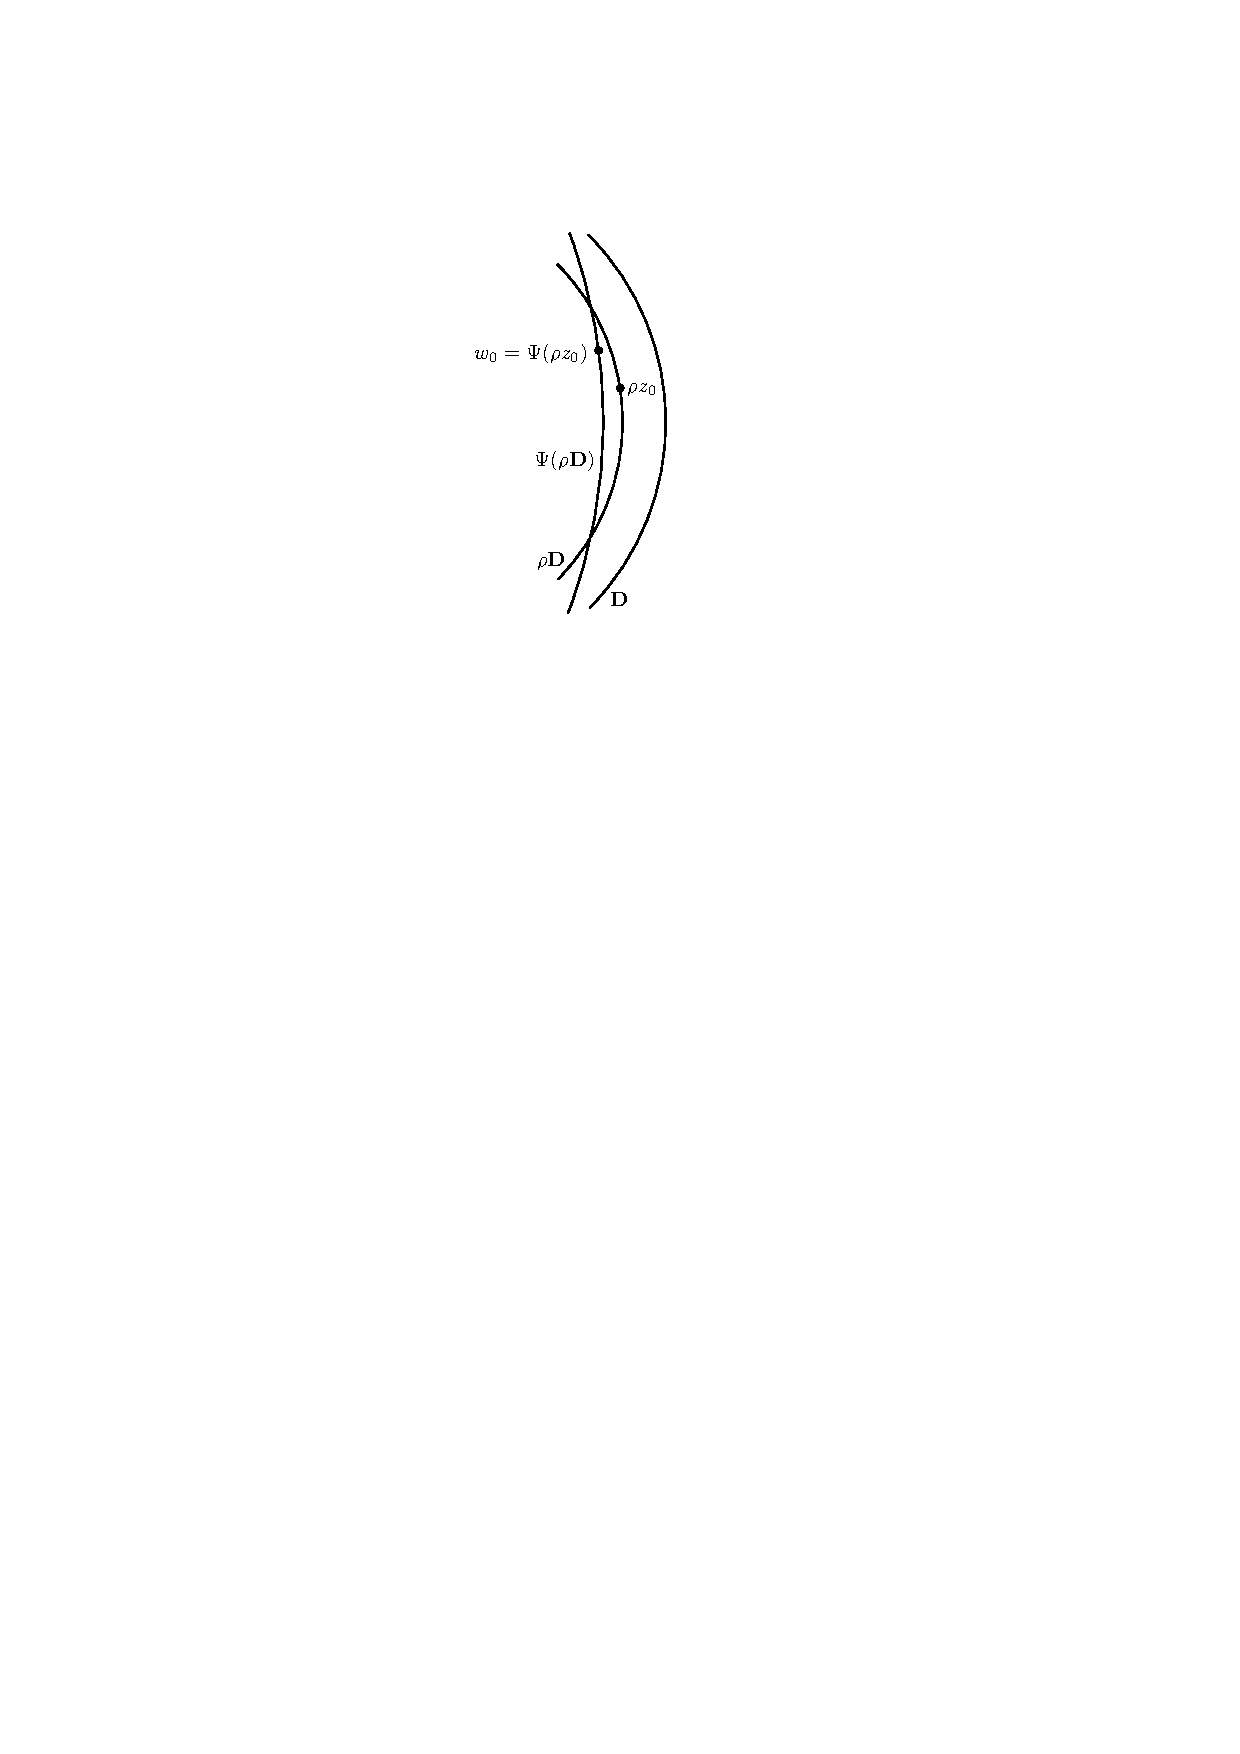
\includegraphics[scale=1]{circles} \\[2ex]
		\caption{Illustration of the points $z_0,w_0\in\C$ defined in the proof
			of Theorem~\ref{th:complex}.  We first choose $z_0 = e^{i\theta}$
			for $|\theta|\leq c_2/L$, such that $|\wt Q(\rho\cdot)|$ is bounded from below.
			Then we observe that $|w_0|<1-c_2/L^2$, which helps us to bound
			the modulus of $\E[\sum_{j\geq 0} \wt a_j w_0^j]$ from below.}
		\label{fig:z_0}
	\end{figure}
	To see this, define $\Pt (z) = z^{-\E S} P(z)$, which is an analytic function in the right half-plane.  For all $z$ in the
	right half-plane satisfying $1 \le |z| \le \rho^{-1}$, differentiating
	$\Pt$ and using $\E [ |S - \E S| ] \le L$ and $d \le L^2$ gives
	\begin{align*}
	|\Pt' (z)|
	& = \left| \sum_{j = 0}^{d} (j - \E S) \sigma(j) z^{j - \E S - 1} \right|
	\le \sum_{j = 0}^{d} |j - \E S|\cdot \sigma(j) \cdot |z|^{j - \E S - 1} \\
	& \le \rho^{-d} \cdot \E[ |S - \E S| ]
	\le \rho^{-d} L \le e^{\frac{1.1 d}{L^2}} \cdot L \le 4L,
	\end{align*}
	%
	We also have
	%
	\begin{align*}
	|\rho^{-1} z_0^{-1} - 1| &= \rho^{-1} |1 - \rho z_0| \le |z_0 - 1|
	+ \rho^{-1}(1 - \rho) \le \frac{c_2}{L}+ \frac{2}{L^2}.
	\end{align*}
	%
	Therefore, for all sufficiently large $m$,
	%
	\begin{align*}
	\left | P(\rho^{-1}z_0^{-1}) \right |
	&= \rho^{-\E S} \left | \wt{P}(\rho^{-1}z_0^{-1}) \right |
	\ge 1 - |\wt{P}(\rho^{-1}z_0^{-1}) - 1| \\
	&= 1 - \left| \int_1^{\rho^{-1}z_0^{-1}} \wt{P}'(z) \,dz \right|
	\ge 1 - |\rho^{-1}z_0^{-1} - 1| \cdot 4L \\
	&\ge 1-\left( \frac{c_2}{L}+ \frac{2}{L^2} \right)\cdot 4L \ge \frac{1}{2} \, ,
	\end{align*}
	proving~\eqref{eq:P}.
	
	Using Lemma \ref{prop15} and the above estimates, it follows that
	\begin{eqnarray} \label{eq8}
	\left | \E \left [ \sum_{j\geq 0} \wt a_j w_0^j \right] \right |
	& \geq & p\cdot \left | P \left ( \frac{1}{\rho z_0} \right ) \right |
	\cdot  \rho^{j_0} \cdot|\Qt (\rho z_0)|\\
	& \geq & p \frac{1}{2} \left ( 1 - \frac{1}{L^2} \right )^m e^{- \cbe L/c_2}
	\nonumber \\
	& \geq & e^{- \csep L} \nonumber
	\end{eqnarray}
	for a constant $\csep > 1$ depending only on $q,q'$.
	%	
	Since $|w_0|\leq 1-c_2/L^2$, for any $\cfwd > 1$,
	\eqb
	\left|\sum_{j\geq \cfwd m} \E[\wt a_j] w_0^j\right|
	\leq
	\left | \sum_{j \geq \cfwd m} \left ( 1 - \frac{c_2}{L^2} \right )^j \right |
	\leq L^2 c_2^{-1} e^{- \cfwd L/c_2} \, .
	\label{eq26}
	\eqe
	%
	Combining \eqref{eq8} and \eqref{eq26}, for $\cfwd$ a sufficiently large constant multiple of $\csep$,
	\eqb
	\begin{split}
		\E\left[ \sum_{j=0}^{\lceil \cfwd m\rceil-1} \left|\wt a_j w_0^j \right|\right]
		\geq
		\left|\E\left[ \sum_{j=0}^{\lceil \cfwd m\rceil-1} \wt a_j w_0^j \right]\right|
		\geq
		\frac 12 \exp(- \csep L).	
	\end{split}
	\eqe
	%
	It follows that there is a $j < \cfwd m$ for which
	$$|\E[\aat_j]| \geq |\E[\aat_j] w_0^j| \geq (2 \lceil\cfwd m\rceil)^{-1}\exp(-\csep L) \, .$$
	Increasing $\csep$ if necessary finishes the proof.
\end{proof}



% Acknowledgments---Will not appear in anonymized version
\acks{We thank Margalit Glasgow for her careful reading and comments.}



\end{document}
